\chapter{Experiments}\label{ch_experiments}

The previous chapter designed a three-level optimisation pipeline - expression-level rewrites, structural passes, and data-level transformations - together with a cumulative ablation methodology for measuring each pass's contribution.
This chapter applies that methodology to evaluate the pipeline empirically.

The evaluation is structured to mirror the pipeline's own architecture.
\cref{sec_exp_expressions} isolates the eight expression-level passes, measuring their effect on style size, load time, and AST complexity in cumulative ablation order.
\cref{sec_exp_structural} evaluates the six structural passes, with particular attention to inter-pass dependencies and the synergy between dead layer elimination and layer merging.
\cref{sec_exp_mlt} assesses data-level optimisations, demonstrating the cascade from style-level dead layer elimination through tile shaving into smaller tiles, and evaluating how the encoding strategy competition delivers the shaved data to the wire.
\cref{sec_exp_cross_style} tests generalisation by applying the full pipeline to 15 styles beyond the deep benchmarking corpus, and \cref{sec_exp_combined} brings all three levels together to quantify the end-to-end effect on tile volume, load time, and rendering stability - and to examine how style-level and data-level optimisations interact through the cascade.

\section{Experiment 1: Expression-Level Optimisations}\label{sec_exp_expressions}

This experiment evaluates the eight expression-level passes described in \cref{sub_expression_optimisations}: unary simplification, expression kind normalisation, constant folding, stats-driven constant folding, expression simplification, default stripping, colour minification, and selectivity reordering.
These passes operate directly on the JSON representation of style expressions, applying peephole rewrites in a fixpoint loop until no further changes are detected.

\subsection{Evaluation}\label{sub_expr_evaluation}

Expression passes are evaluated in cumulative ablation order: unary simplification, expression kind normalisation, constant folding, stats-driven constant folding, expression simplification, default stripping, colour minification, and selectivity reordering.
The first seven passes correspond to ablation steps~1-7 in the benchmark harness.
Selectivity reordering (step~16) is evaluated separately as it requires tile statistics.

Metrics reported include style size (raw, gzip, Brotli), load time, frames per second, frame time percentiles, and \ac{AST} complexity (node count, maximum depth).

\subsection{Results}\label{sub_expr_results}

\cref{fig:waterfall_loadMs} shows the cumulative effect of adding each expression pass in ablation order on median load time, aggregated across the full scenario corpus; lower bars mean a shorter end-to-end load.
\cref{fig:marginal_loadMs} then isolates the \emph{marginal} contribution of each pass, stripping out the cumulative accumulation so that individual passes can be compared on a level footing.
Read together, the two views separate \enquote{which passes are pulling their weight} from \enquote{how much does the stack as a whole improve over the baseline}.

Across the benchmark corpus, the seven expression passes reduce the median load time from \qty{424}{\milli\second} (baseline) to \qty{416}{\milli\second} (\qty{-1.8}{\percent}).
Per-style bootstrap confidence intervals show that this aggregate effect is not consistently significant for individual styles - the style-level load-time signal is small relative to measurement noise, and for some styles the median shifts in the opposite direction.
The primary value of expression passes is therefore not a direct load-time reduction but the \emph{enabling effect} on downstream structural and data-level passes (discussed in \cref{sub_structural_interactions}).
The single largest marginal contributor is expression simplification (step~5), which accounts for \qty{-9.3}{\milli\second} (\qty{-2.2}{\percent}) by collapsing nested boolean logic and rewriting multi-arm case expressions into more compact match forms.
The size effect is more pronounced than the rendering effect: Fiord's raw style shrinks by \qty{20.3}{\percent} (\num{22215}$\to$\qty{17707}{\byte}), while Liberty - already compact in its expression usage - shrinks by \qty{7.0}{\percent} (\num{43060}$\to$\qty{40056}{\byte}).
Under gzip, the reductions are \qty{8.3}{\percent} and \qty{5.9}{\percent} respectively, confirming that some of the raw-byte savings are absorbed by the compressor.

\begin{figure}[htbp]
    \centering
    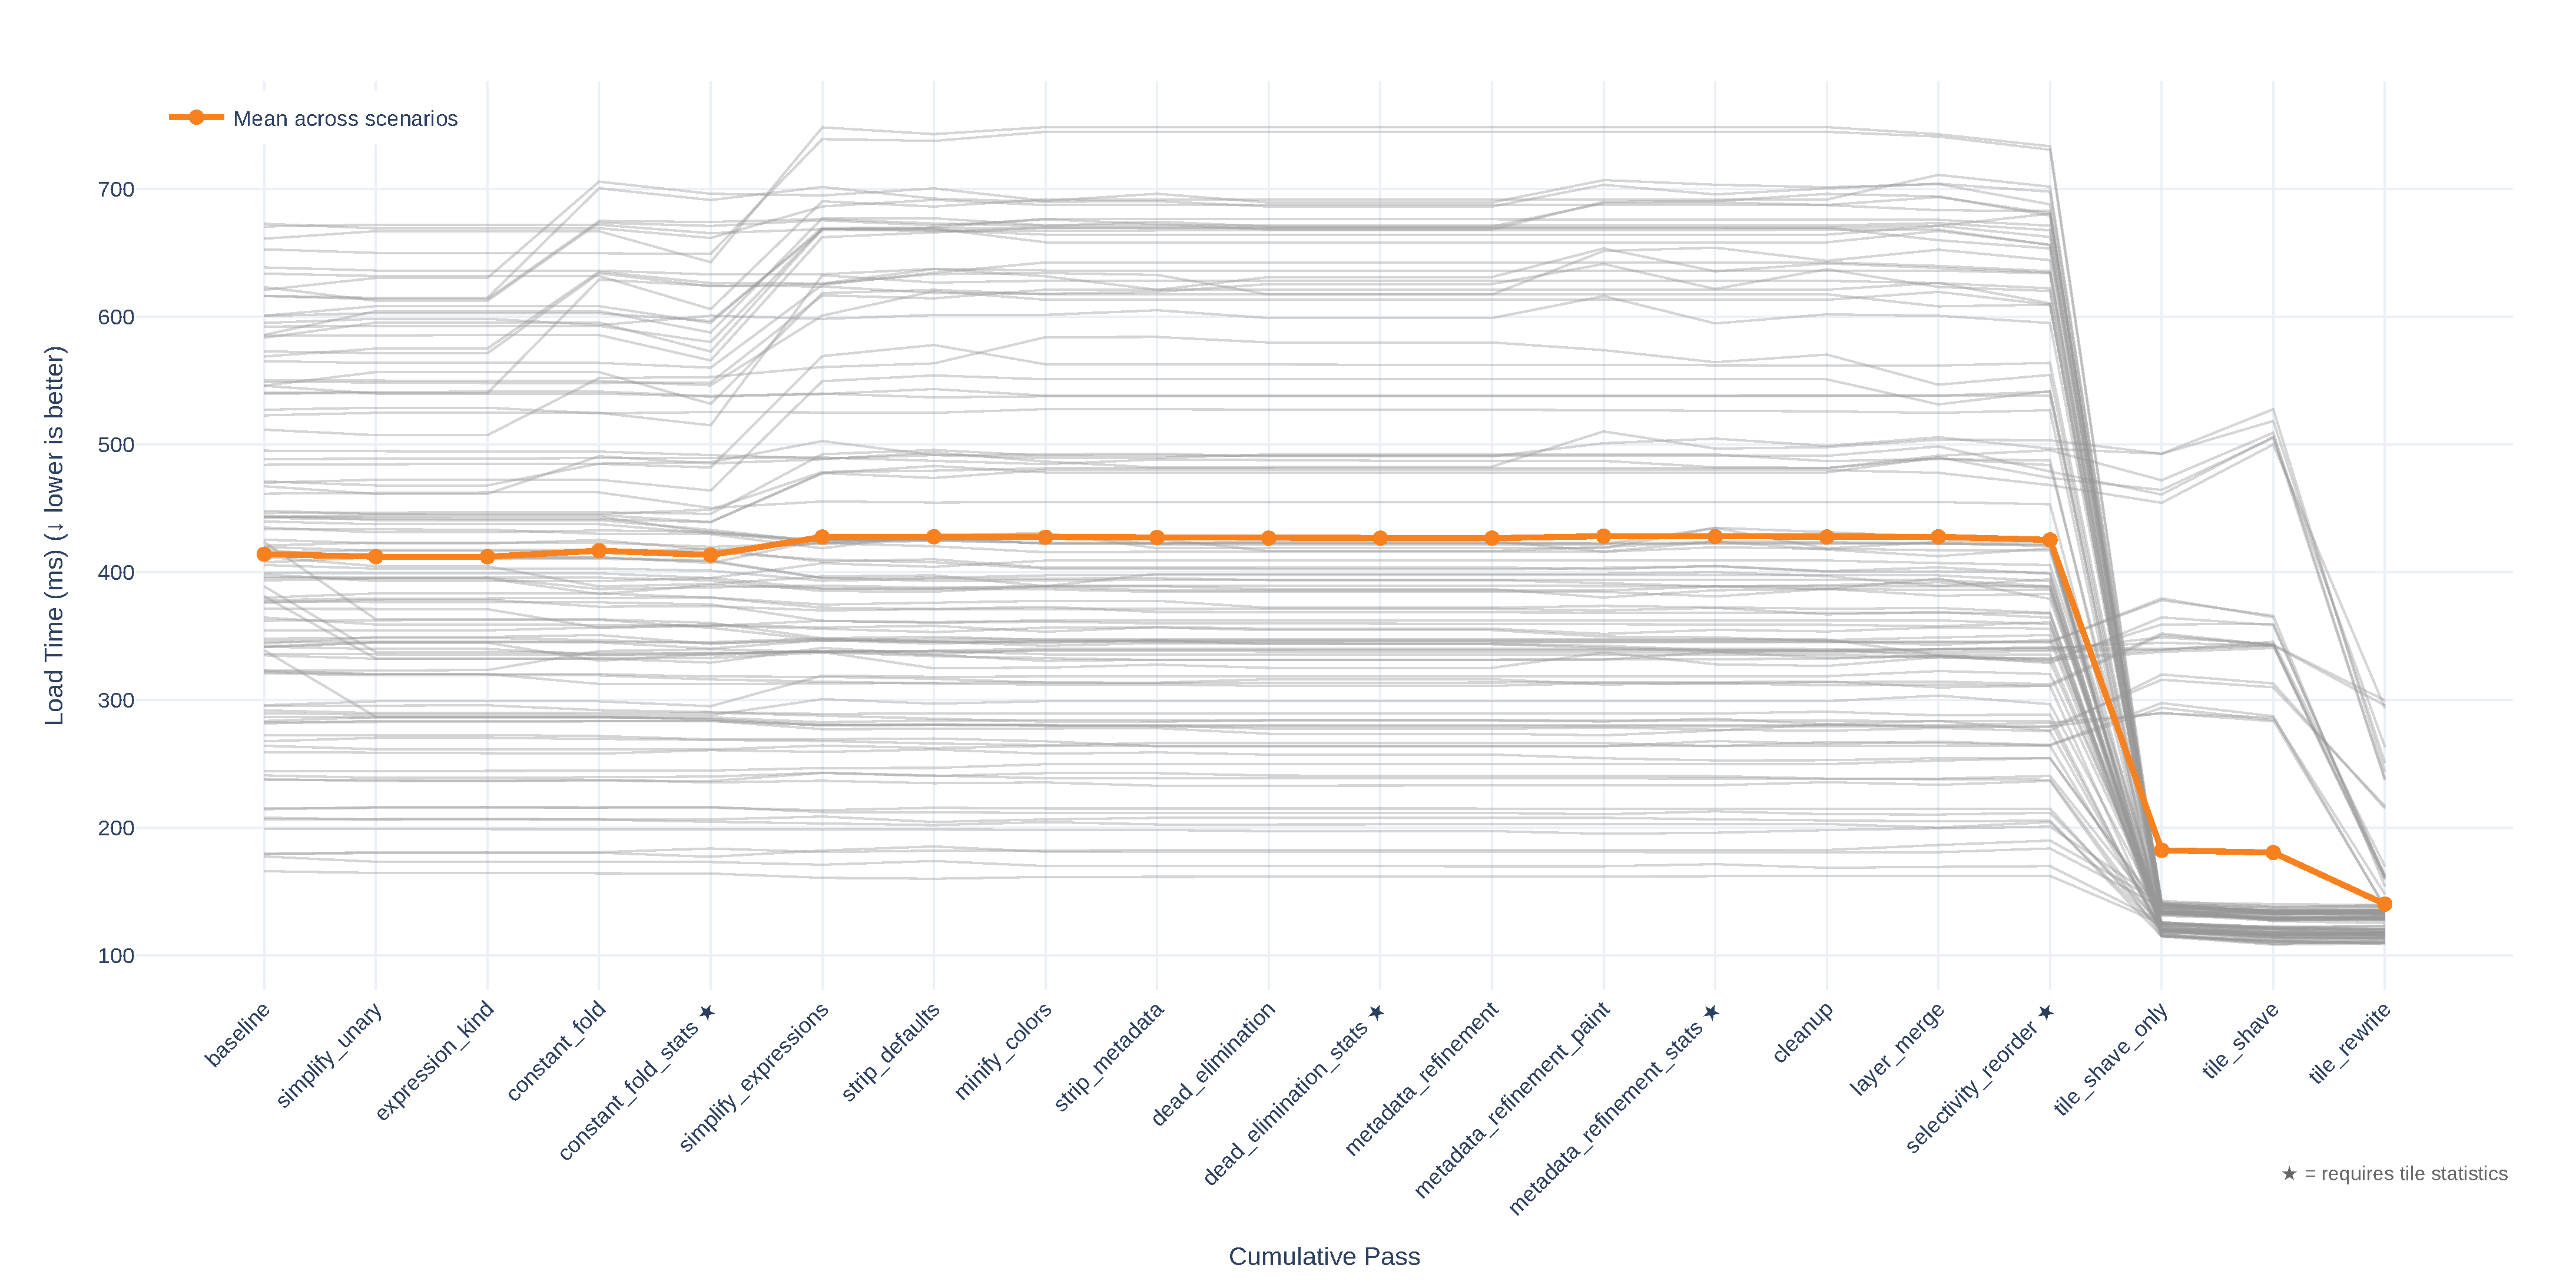
\includegraphics[width=\linewidth]{figures/waterfall_loadMs.pdf}
    \caption{Cumulative ablation waterfall for load time. Each bar shows the median change introduced by adding one expression pass on top of all previous passes, aggregated across all 18 scenarios and 15 benchmark styles}
    \label{fig:waterfall_loadMs}
\end{figure}

\begin{figure}[htbp]
    \centering
    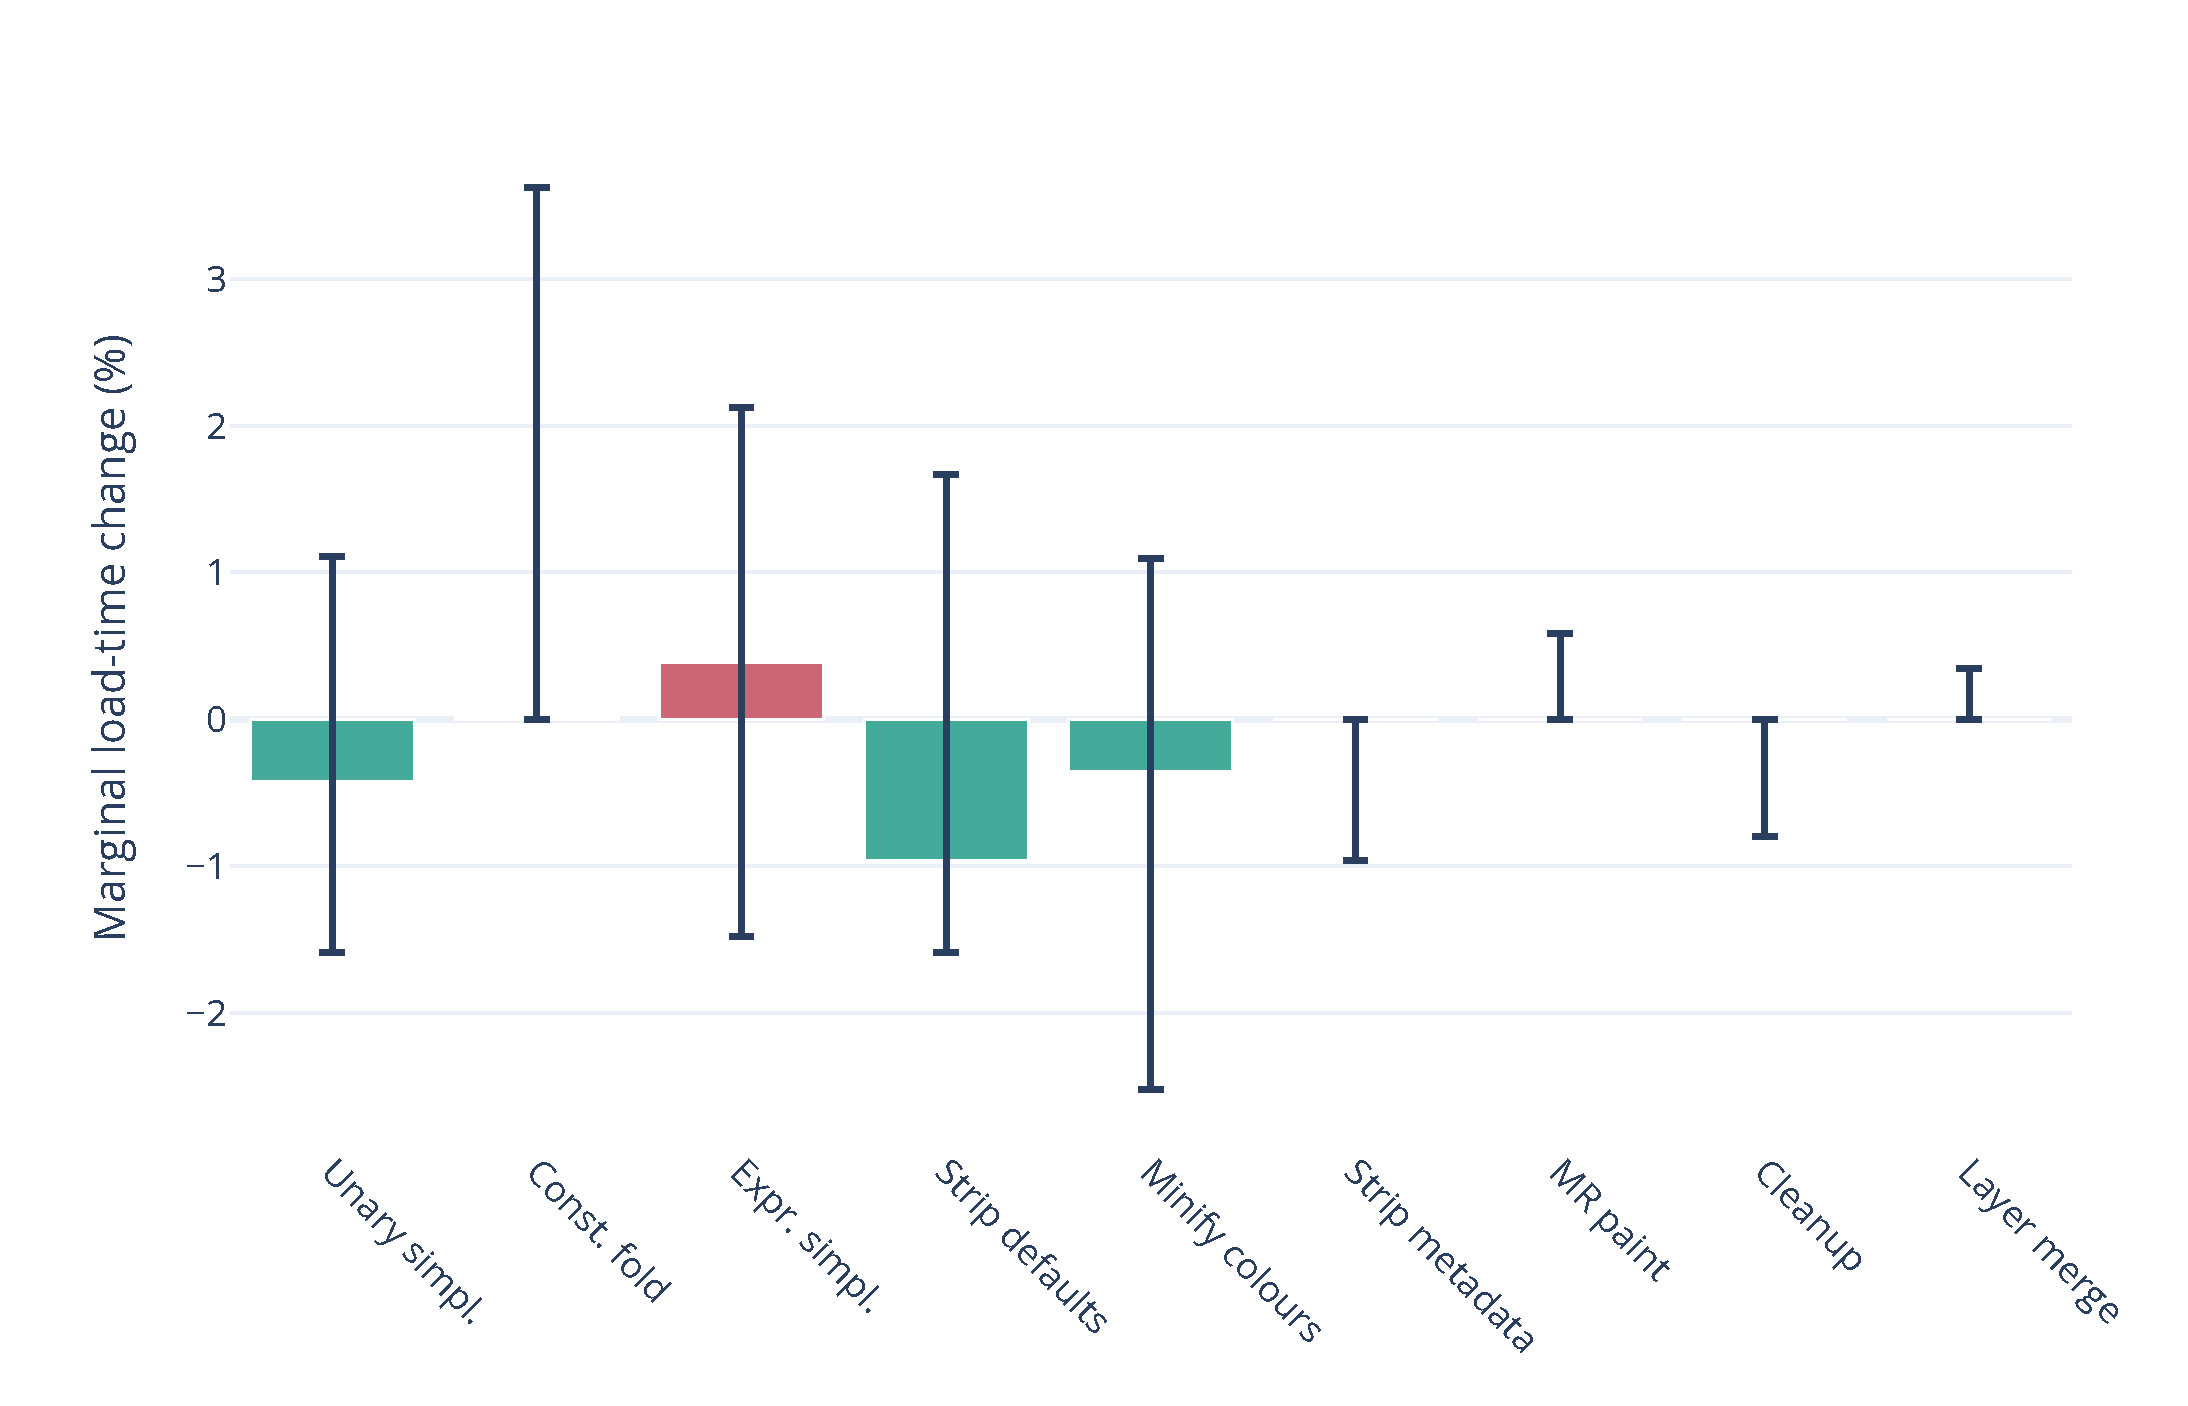
\includegraphics[width=\linewidth]{figures/marginal_loadMs.pdf}
    \caption{Marginal contribution of each expression pass to load time reduction}
    \label{fig:marginal_loadMs}
\end{figure}

\subsection{Discussion}\label{sub_expr_discussion}

Several observations emerge from the expression-level ablation.

\paragraph{Constant folding dominates}
Among the seven expression passes, constant folding and stats-driven constant folding consistently produce the largest marginal improvements.
This is expected: reducing an expression to a literal eliminates all per-feature evaluation cost for that expression, whereas algebraic simplifications merely shorten the evaluation path.
The effect is amplified by fixpoint iteration: a single successful fold can cascade through nested expressions, collapsing entire subtrees in subsequent iterations.

\paragraph{Size reduction vs.\ rendering improvement}
Passes that primarily reduce serialised style size - default stripping, colour minification - show smaller rendering improvements but contribute meaningfully to transfer size under compression.
This primarily benefits time to first render (discussed in \cref{sub_combined_marginal}).
The distinction between raw, gzip, and Brotli reductions is notable: some rewrites (e.g., \texttt{any}$\to$\texttt{in}) increase raw token count while decreasing compressed size, because the repetitive structure of \texttt{in} operand lists compresses well.

\paragraph{Fixpoint convergence}
Confirming the design expectation (\cref{sub_pipeline}), all styles converged within two to three fixpoint iterations.
Styles with deeply nested expressions (e.g., Americana, which uses complex label logic) sit at the upper end of this range.

\paragraph{Stats-driven passes require full coverage}
Stats-driven constant folding is gated on a sample rate of~$1.0$ for folding operations, since removing an expression arm based on incomplete data could produce incorrect rendering.
Frequency-based reordering, however, is safe under sampling, as the relative ordering of selectivities is robust to moderate sampling noise.

\paragraph{Downstream cascade into the data pipeline}
Beyond their direct rendering benefit, expression-level simplifications cascade into the data-level pipeline evaluated in \cref{sec_exp_mlt}.
Each folded filter predicate and each pruned \texttt{match} arm reduces the set of property names and categorical values that the tile pruning advisory (\cref{sub_tile_shaving}) must track; each filter reduced to \texttt{false} enables dead layer elimination in the structural phase, which removes that layer's entire property footprint from the advisory.
Simpler filters are also more amenable to the advisory's static analysis, because canonical forms (e.g., a direct \texttt{["==",~\ldots]} rather than a double-negated comparison) expose referenced property values more readily.
The magnitude of this cascade is quantified in \cref{sec_exp_mlt}.


\section{Experiment 2: Structural Optimisations}\label{sec_exp_structural}

This experiment evaluates the structural passes described in \cref{sub_structural_optimisations}: metadata stripping, dead layer and source elimination (with and without tile statistics), metadata refinement (from filters, paint ramps, and tile statistics), cleanup, and layer merging.
These passes operate on typed Rust structures generated from the upstream MapLibre style specification, enabling transformations that require cross-layer or cross-source reasoning.

\subsection{Pass Interactions}\label{sub_structural_interactions}

The ordering of structural passes is significant, and several inter-pass dependencies constrain the feasible orderings.

\paragraph{Expression passes precede structural passes}
\begin{sloppypar}
Metadata refinement relies on zoom predicates appearing in canonical form - e.g., \texttt{[">=",\allowbreak{} ["zoom"],\allowbreak{} 10]} rather than \texttt{["!",\allowbreak{} ["<",\allowbreak{} ["zoom"],\allowbreak{} 10]]}.
The expression simplification pass (De~Morgan, double-negation elimination) normalises such patterns, and constant folding may collapse compound zoom guards into a single predicate.
Without this normalisation, the metadata refinement pass would fail to recognise many zoom predicates.
\end{sloppypar}

\paragraph{Dead elimination before layer merging}
A dead layer (filter reduced to \texttt{false}) between two mergeable live layers prevents the merging pass from recognising them as adjacent candidates.
By running dead elimination first, the gap is closed and the live layers become merge-eligible.
This interaction is one reason why the cumulative ablation reveals a larger marginal contribution for layer merging when dead elimination is already active.

\paragraph{Metadata refinement before cleanup}
Metadata refinement may lift a zoom predicate out of a filter, leaving the filter as \texttt{true}.
It may also tighten zoom bounds such that a layer with a zero-to-nonzero opacity ramp becomes invisible across its entire zoom range.
Cleanup removes these residual artefacts.

\paragraph{Fixpoint re-fold after structural changes}
Structural passes remove filter predicates (e.g., zoom guards consumed by metadata refinement), which can leave behind wrapper expressions such as \texttt{["all",~x]} or \texttt{["any",~x]}.
A final expression re-fold pass collapses these to the bare \texttt{x}, ensuring the serialised style is clean.

\paragraph{Layer merging last}
Layer merging is placed after all other structural passes to maximise the pool of mergeable candidates.
Dead elimination removes blockers; metadata refinement may make zoom ranges identical (enabling direct merging rather than zoom-tolerant merging); cleanup removes invisible layers that would otherwise occupy adjacency slots.

\subsection{Evaluation}\label{sub_structural_evaluation}

Structural passes correspond to ablation steps~8-15: metadata stripping, dead elimination, dead elimination with statistics, metadata refinement, metadata refinement via paint ramps, metadata refinement with statistics, cleanup, and layer merging.

In addition to the rendering metrics used for expression passes, the structural evaluation reports complexity metrics: layer count, filter count, and total expression node count.

\subsection{Results}\label{sub_structural_results}

\cref{fig:complexity_layer_count} tracks layer count across the structural ablation steps, showing which passes concretely remove layers rather than merely rewriting them.
\cref{fig:style_size_ablation} complements this with the raw, gzip, and Brotli style sizes, confirming that a reduction in layer count also translates into a reduction in transfer size and not just a reshuffling of the serialised form.

The magnitude of structural improvement is style-dependent.
Fiord's layer count drops from 48 to 46 (\qty{-4.2}{\percent}), with dead elimination removing one layer (step~9) and cleanup removing another (step~14) after metadata refinement lifts zoom predicates that leave a filter as \texttt{true} on an invisible layer.
Liberty's layer count drops from 111 to 107 (\qty{-3.6}{\percent}), concentrated entirely in the layer-merge step (step~15), which merges four pairs of adjacent layers with compatible filters.
In terms of gzip transfer size, Fiord benefits substantially (\qty{-14.1}{\percent} from baseline to step~15), while Liberty sees a modest \qty{-4.9}{\percent}, with layer merging slightly \emph{increasing} gzip by \qty{36}{\byte} due to the larger merged filter expressions.
AST complexity tells a similar per-style story: Fiord's expression nodes drop by \qty{36.8}{\percent} (\num{1610}$\to$\num{1018}), whereas Liberty's drop by \qty{10.5}{\percent} (\num{3537}$\to$\num{3167}).

\begin{figure}[htbp]
    \centering
    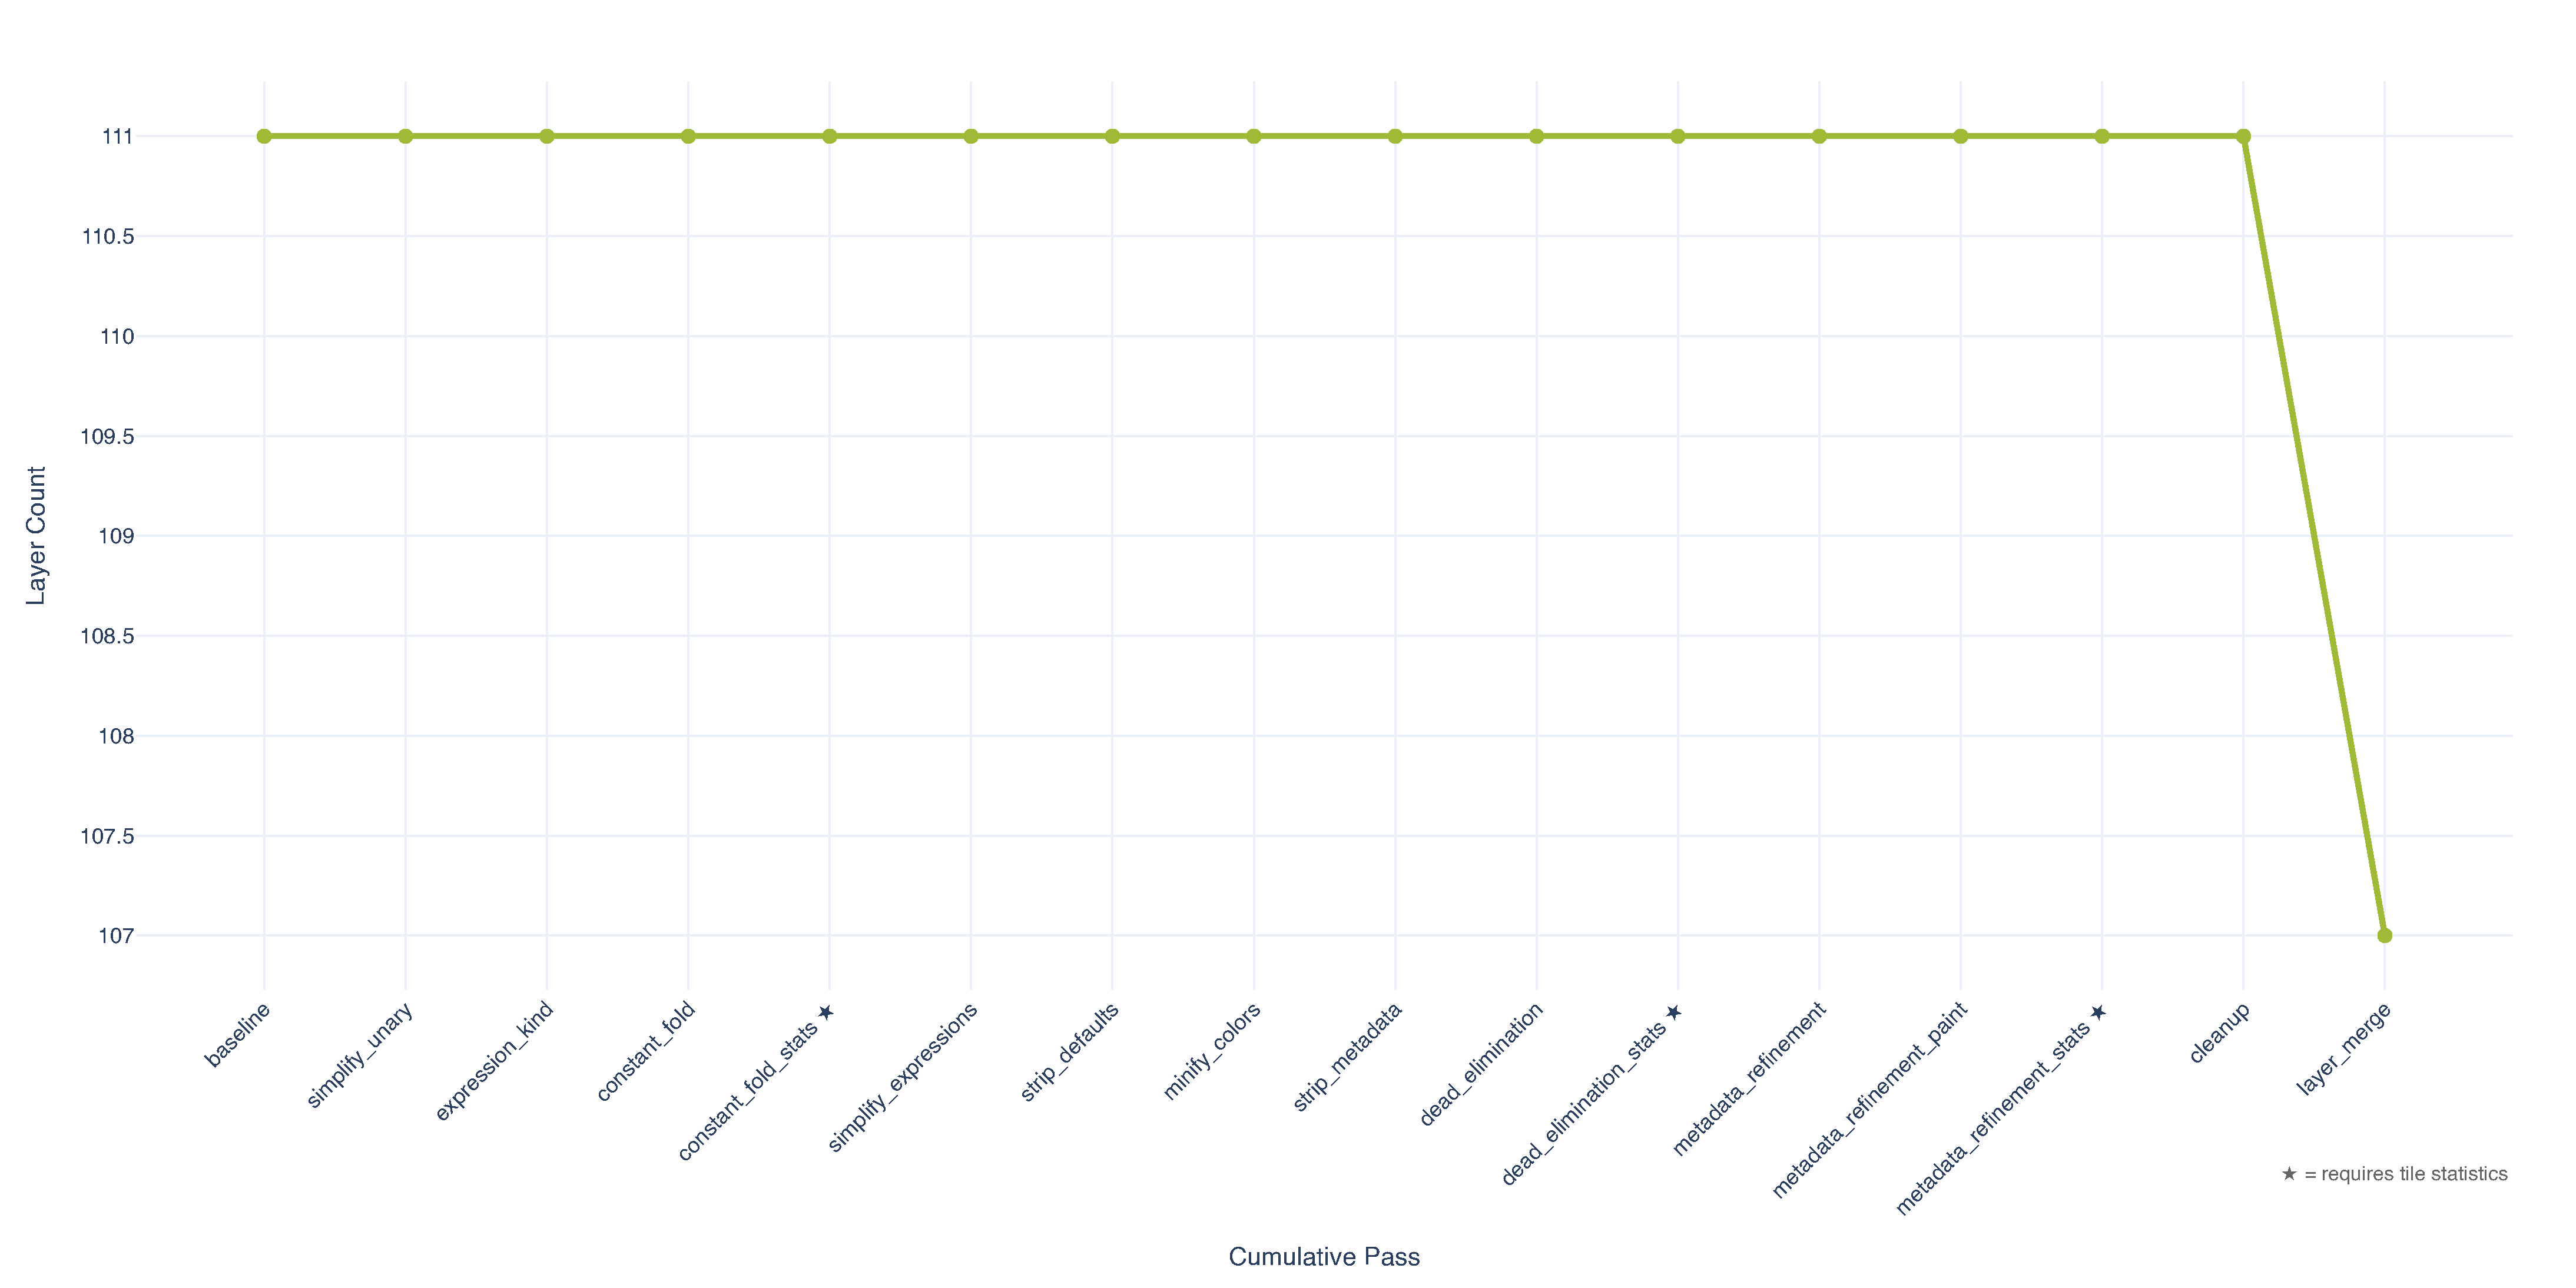
\includegraphics[width=\linewidth]{figures/complexity_layer_count.pdf}
    \caption{Layer count across cumulative ablation steps on the liberty style showing a representative behavior that only layer merging reduces the amount of layers. Dead elimination usually is unable to entirely remove layers because styles are usually designed to show parts of the map and thus cannot be safely removed.}
    \label{fig:complexity_layer_count}
\end{figure}

\begin{figure}[htbp]
    \centering
    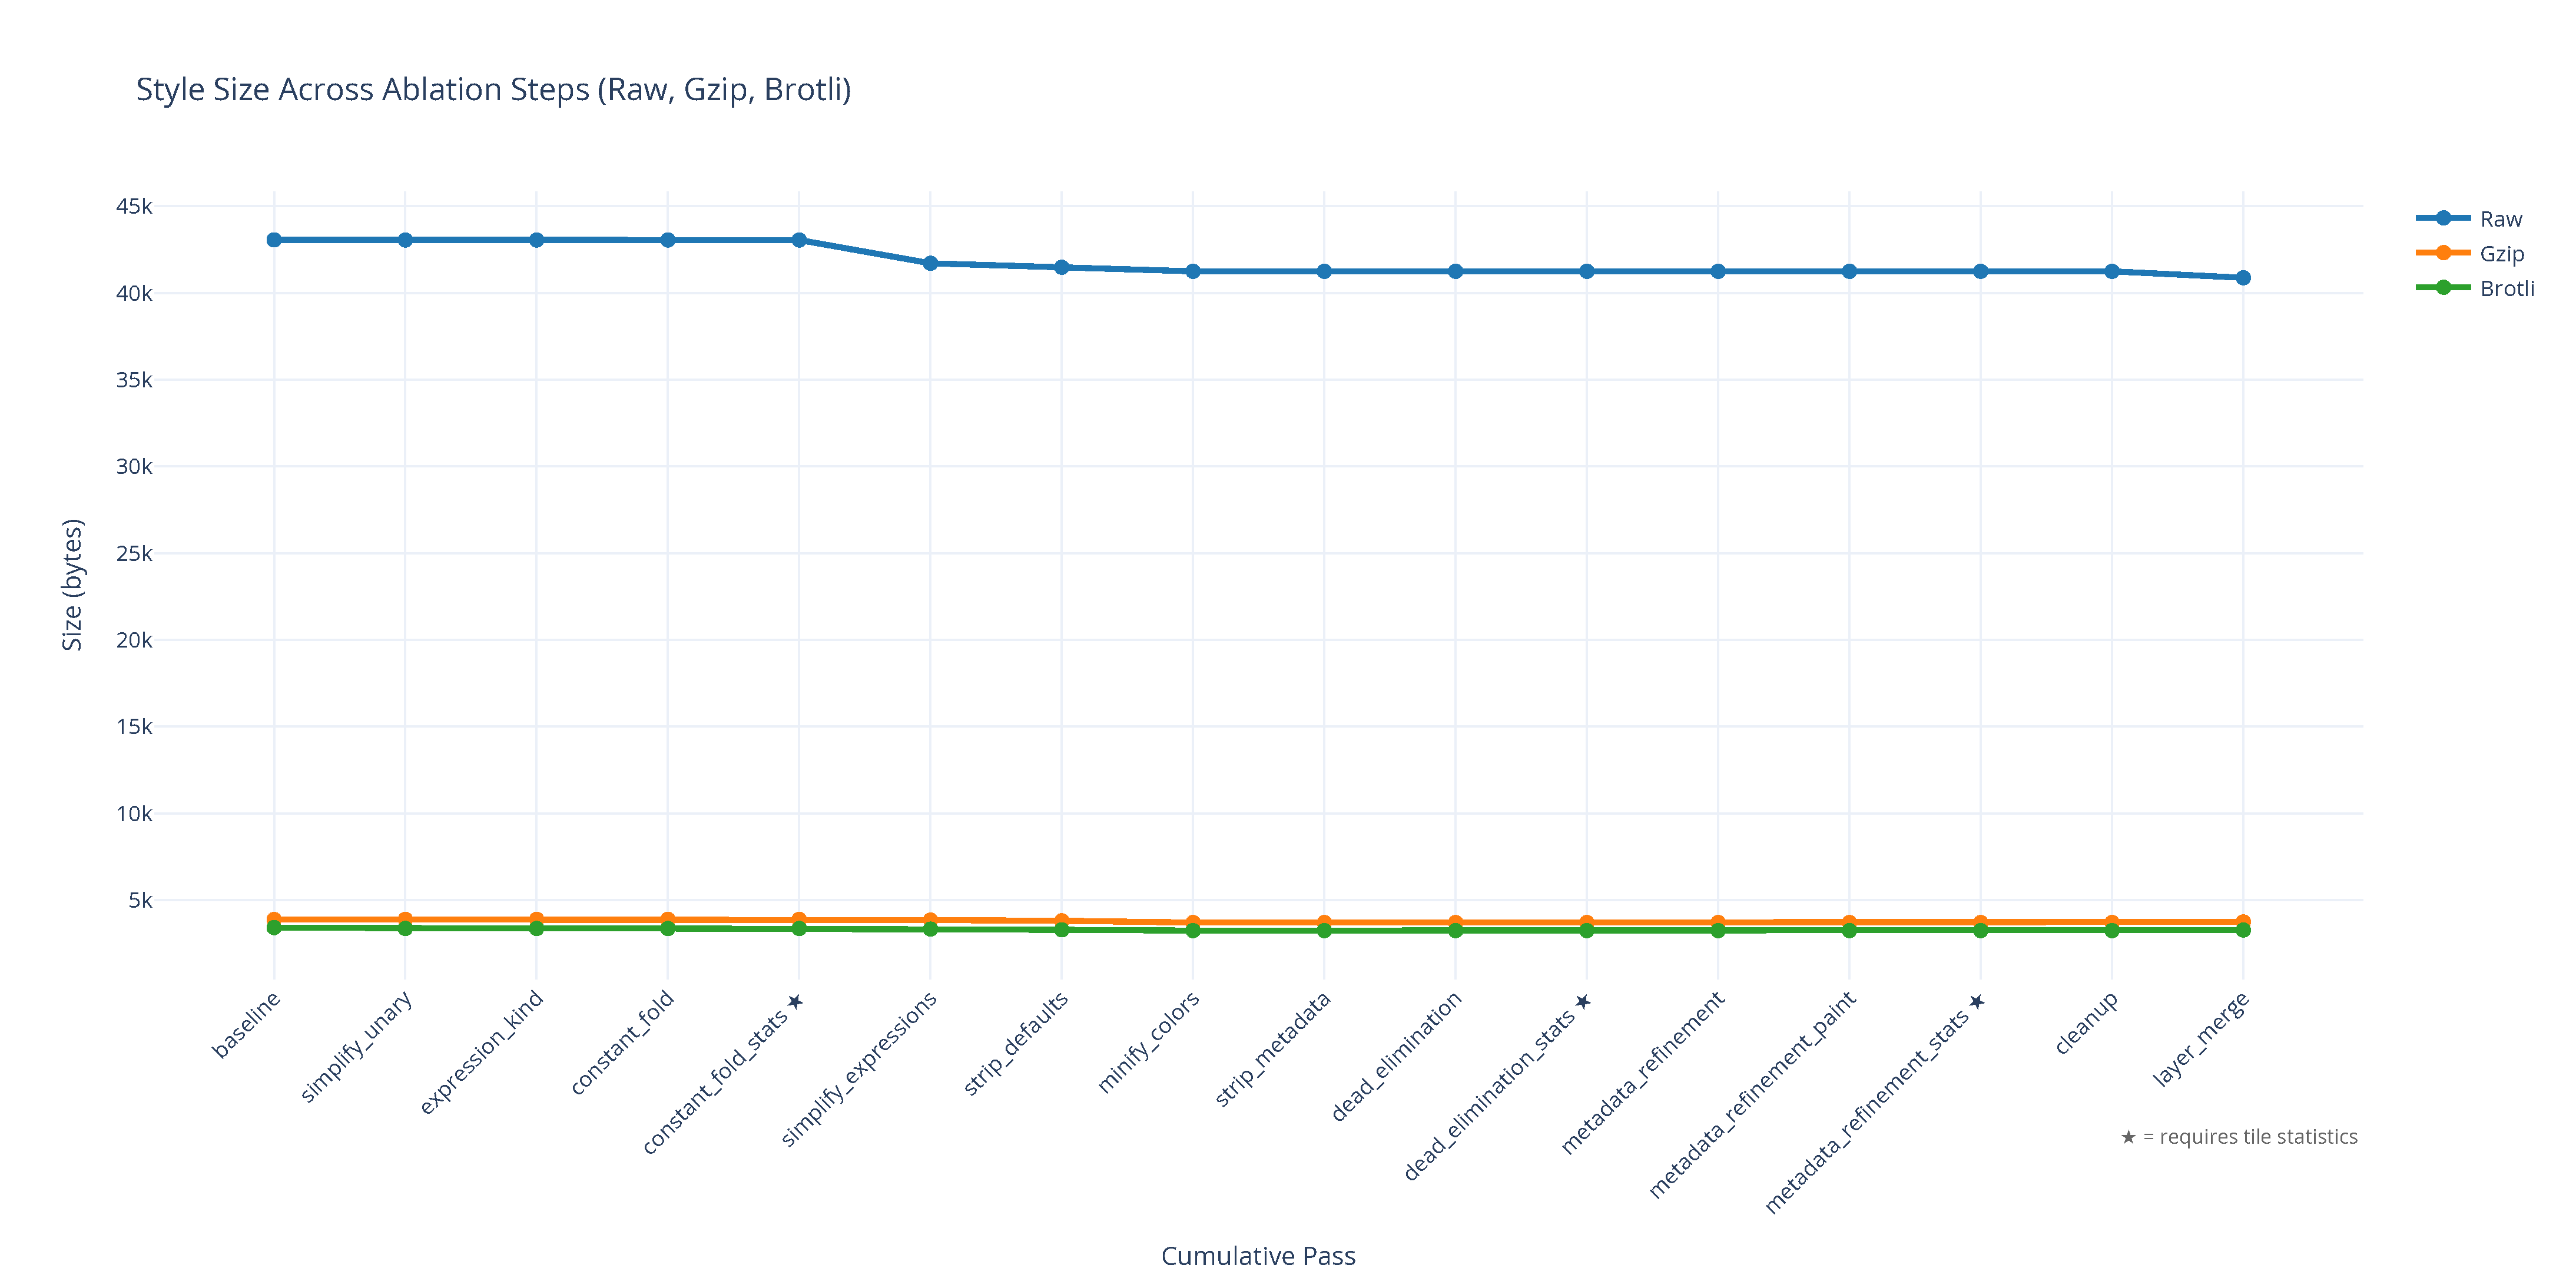
\includegraphics[width=\linewidth]{figures/style_size_ablation.pdf}
    \caption{Style size (raw, gzip, Brotli) across ablation steps}
    \label{fig:style_size_ablation}
\end{figure}

\subsection{Discussion}\label{sub_structural_discussion}

\paragraph{Dead elimination and layer merging dominate}
Among the structural passes, dead elimination and layer merging produce the largest improvements in both rendering performance and style complexity.
Dead elimination directly reduces the number of layers the renderer must process per frame; layer merging reduces draw calls by combining multiple rendering passes into one.
The interaction between the two is synergistic: styles with many narrowly-filtered layers (e.g., road styles that define separate layers for each road class) benefit most, as dead elimination first removes layers for road classes absent from the data, and layer merging then combines the remaining layers into a single multi-class layer.

\paragraph{Layer merging can trade raw size for runtime savings}
Layer merging does not always reduce the raw serialised byte count: a merged layer replaces $k$ small filter expressions with a single \texttt{match}-keyed filter and $k$-armed \texttt{match} expressions for every differing paint property, which for small $k$ can produce a slightly larger textual representation than the sum of the originals.
The per-style ablation tables in \cref{app_per_style} show one such case (OSM Liberty: \num{27628}$\to$\qty{28328}{\byte} after layer merging), where the raw count increases while the layer count drops from 105 to 103.
The important observation is that raw byte count is a proxy metric for parse time and transfer cost, whereas the driver of rendering performance is layer count and per-frame draw calls; the merged layer is still cheaper to render even when its serialised form is larger.
The gzip and Brotli columns of the same table show that the compressed size is essentially unchanged, confirming that the raw increase disappears under realistic wire compression.

\paragraph{Metadata refinement has indirect effects}
Metadata refinement does not directly reduce the number of layers or the complexity of expressions; instead, it enables the renderer to skip layers at zoom levels where they are invisible.
The rendering improvement is therefore zoom-dependent: at overview zoom levels (where many layers are filtered out by tightened \texttt{minzoom}), the improvement is large; at street-level zoom (where most layers are active), the improvement is smaller.
Paint-based refinement captures a class of optimisations that are invisible to filter analysis - a layer whose opacity interpolates from~0 at zoom~12 is indistinguishable from a fully visible layer when examining only the filter.

\paragraph{Stats-driven passes amplify style-only passes}
The marginal contribution of stats-driven dead elimination (step~10) over non-stats dead elimination (step~9) quantifies the value of tile statistics for style optimisations.
Styles that use broad \texttt{source-layer} references benefit most, as statistics reveal which geometry types and property values actually exist.
For styles that already have precise filters (e.g., hand-tuned Americana), the marginal gain is smaller.

\paragraph{Symbol layer exclusion}
The decision to exclude symbol layers from merging is conservative but necessary.
MapLibre's label collision detection operates per-layer: labels within the same layer compete for screen space, while labels in different layers are resolved separately.
Merging two symbol layers would change which labels collide, potentially hiding labels that the original style intended to show or showing labels that should have been suppressed.
A future extension could detect cases where merged symbol layers produce identical collision behaviour, but this would require modelling the collision algorithm, which is beyond the scope of this work.

\paragraph{Downstream cascade into tile shaving}
Dead layer elimination has a second-order effect beyond reducing per-frame draw calls: each eliminated layer removes its property references from the tile pruning advisory computed in the data-level pipeline (\cref{sub_tile_shaving}).
If a removed layer was the sole consumer of a property column, that column is stripped from every tile at encoding time.
Similarly, metadata refinement's tightened zoom bounds cause the advisory to mark additional zoom levels as unused for a given source-layer, potentially eliminating entire tiles.
This cascade is the thesis's central architectural finding; it is characterised fully in \cref{sub_mlt_discussion} and quantified in \cref{sub_mlt_results}.


\section{Experiment 3: Data-Level Optimisations}\label{sec_exp_mlt}

Experiments~1 and~2 optimised the \emph{program} the renderer executes: simpler expressions, fewer layers, tighter metadata.
Each of these style-level changes also narrows the set of tile data that the rendering pipeline references - an effect that the preceding discussions identified as a cascade from style optimisation through the tile pruning advisory into smaller tiles.
This experiment asks: can the \emph{data} itself be co-optimised to exploit this cascade, and does the predicted interaction between style-level and data-level optimisations actually materialise?

The research by Tremmel et al.~\cite{tremmelMapLibreTileNext2025} demonstrated that the \ac{MLT} columnar format is structurally superior to protobuf-based \ac{MVT}, offering columnar storage, built-in compression, and a richer type system.
However, their evaluations used fixed encoder configurations that did not consider the characteristics of the data being encoded, and did not consider the style.
This experiment bridges that gap by applying the data-level pipeline described in \cref{sub_data_optimisations} - style-driven tile shaving, data transformations, and automatic encoding strategy selection - using the optimised style from Experiments~1--2 to drive the pruning advisory.

\subsection{Problem Statement}\label{sub_mlt_problem}

Two problems remain open after the style-level optimisations of Experiments~1 and~2:

\begin{enumerate}
    \item \textbf{Tiles carry data the style never uses - and how much depends on the style.}
    Vector tiles are produced from a general-purpose schema (e.g., OpenMapTiles) that includes hundreds of properties and multiple geometry types.
    A specific rendering style references only a fraction of these.
    Crucially, the amount of removable data is \emph{style-dependent}: a style with many dead layers (removed by Experiment~2's dead elimination) references fewer properties, leaving more columns removable; a style whose expressions have been simplified (Experiment~1) exposes fewer categorical values in its filters, leaving more features removable.
    Unused columns and features are transferred, decoded, and discarded on every tile request - wasted bandwidth and CPU that the style optimisations have made quantifiable.

    \item \textbf{Encoders ignore the data characteristics that shaving produces.}
    Existing \ac{MLT} encoders apply uniform encoding strategies across all columns, disregarding the statistical properties of individual fields.
    After style-driven shaving removes columns and features, the remaining data has different statistical properties: fewer distinct property values (longer \ac{RLE} runs), more homogeneous distributions (better delta encoding), and smaller string vocabularies (more effective dictionary compression).
    An encoder that adapts to these changed characteristics - through the profiler-driven candidate pruning described in \cref{sub_encoding_strategies} - can capture savings that a fixed-strategy encoder leaves on the table.
    Furthermore, safety-critical libraries such as FastPFor~\cite{lemireDecodingBillionsIntegers2015} explicitly disclaim input validation, necessitating the multi-layer correctness validation described in \cref{sub_data_optimisations}.
\end{enumerate}

\subsection{Evaluation Design}\label{sub_mlt_evaluation}

This experiment evaluates the data-level pipeline described in \cref{sub_data_optimisations}: style-driven tile shaving (\cref{sub_tile_shaving}), data transformations (\cref{sub_data_transforms}), and automatic encoding strategy selection (\cref{sub_encoding_strategies}).
The central question is whether style-level and data-level optimisations \emph{compose} - that is, whether optimising the style first and then encoding the resulting tile set produces measurably better results than either optimisation category in isolation.
This directly addresses Research Goal~R1.

The evaluation uses a cumulative design with five configurations, each adding one optimisation layer:

\begin{enumerate}
    \item \textbf{\ac{MVT} baseline}: unoptimised protobuf-encoded tiles served with the original style.
    \item \textbf{Style-only}: the optimised style from Experiments~1-2, served with unmodified \ac{MVT} tiles.
    \item \textbf{Shaving-only}: the original style with tile shaving applied (advisory-driven pruning of unused columns, geometry types, and property values), but without style optimisations.
    \item \textbf{Style + shaving}: the optimised style driving tile shaving - the cascade configuration where dead layer elimination and metadata refinement reduce the advisory, which in turn reduces tile size.
    \item \textbf{Style + shaving + MLT encoding}: the full pipeline - the encoding stage that delivers the shaved data to the wire via automatic encoding strategy selection (sort competition, per-stream profiling, string compression).
\end{enumerate}

\noindent Configurations~2-4 isolate the interaction effect: if the combined reduction of style+shaving exceeds the sum of style-only and shaving-only, the two optimisation categories are \emph{synergistic}; if less, they are partially redundant.
Configuration~5 adds the encoding layer: after shaving has determined what data survives, the multi-strategy competition adapts to the statistical properties of the surviving data - properties that differ from the unshaved original because shaving has removed columns and features, altering value distributions and run-length characteristics.

For each configuration, two classes of metrics are collected: \emph{tile transfer metrics} - encoded tile size (raw, gzip, Brotli) per zoom level, total tileset volume, and encoding time per tile - and \emph{rendering metrics} shared with Experiments~1-2 (load time, frames per second, frame time percentiles p50/p95/p99, and time to first tile), enabling direct comparison of data-level contributions against expression-level and structural contributions in the combined analysis (\cref{sec_exp_combined}).

The tileset covers OpenMapTiles zoom levels~0-14.
Sparse overview tiles at low zoom exercise the advisory's zoom-level pruning; dense urban tiles at high zoom exercise the encoding competition's spatial sorting and per-stream profiling.

\subsection{Results: Style-Driven Cascade}\label{sub_mlt_results}

The central finding of this experiment is the style-to-data cascade previewed in \cref{sub_structural_discussion}: style-level optimisations narrow the pruning advisory, yielding measurably smaller tiles.
The following paragraphs quantify this cascade before turning to the encoding evaluation.

\paragraph{Interaction between style and data optimisations}
\cref{fig:interaction_plot} compares the gzip-size reductions of style-only (config~2), shaving-only (config~3), and their combination (config~4).
For Fiord, the style-only reduction is \qty{14.1}{\percent} and shaving-only contributes a negligible reduction, yet the combined style+shaving reduction is \qty{14.7}{\percent} - the cascade effect of dead-layer elimination shrinking the pruning advisory.
For Liberty, shaving-only also contributes negligibly (Liberty's broad layer structure already references most tile properties), and the combined reduction (\qty{4.8}{\percent}) is close to the style-only reduction (\qty{4.9}{\percent}), indicating approximately additive behaviour.
The aggregate across both styles shows no super-additive interaction at the median level, though per-scenario synergy is present in 16 of the 26 scenarios with complete data.

\paragraph{Rendering metrics across configurations}
\cref{fig:rendering_metrics_mlt} reveals that the dominant rendering improvement comes from tile shaving, not from style optimisations.
The median load time drops from \qty{424}{\milli\second} (baseline) to \qty{406}{\milli\second} with style-only (\qty{-4.1}{\percent}), but plunges to \qty{121}{\milli\second} with shaving-only (\qty{-71.5}{\percent}) and \qty{113}{\milli\second} with style+shaving (\qty{-73.3}{\percent}).
The \ac{MLT} re-encoding step (config~5) adds a small load-time regression relative to config~4 (\qty{119}{\milli\second} vs.\ \qty{113}{\milli\second}, \qty{+5}{\percent}) while achieving better compression (gzip \qty{-11.0}{\percent} vs.\ baseline across both styles).
\ac{FPS} follows the same pattern: shaving-only lifts the median from 807 to \num{2289} (\qty{+184}{\percent}), with style+shaving reaching \num{2331} (\qty{+189}{\percent}).
The \ac{MLT} variant is slightly below at \num{2232} \ac{FPS}, consistent with the additional decoding cost of the columnar format offsetting the smaller transfer size during sustained rendering.
Bootstrap \qty{95}{\percent} confidence intervals confirm that the full-pipeline load-time improvements are tight: Fiord's final load time is \qty{108.7}{\milli\second} (CI: [\num{107.6}, \num{109.7}]), Liberty's is \qty{123.5}{\milli\second} (CI: [\num{122.7}, \num{124.4}]), both with $p < 10^{-45}$ (Wilcoxon) against their respective baselines.

\begin{figure}[htbp]
    \centering
    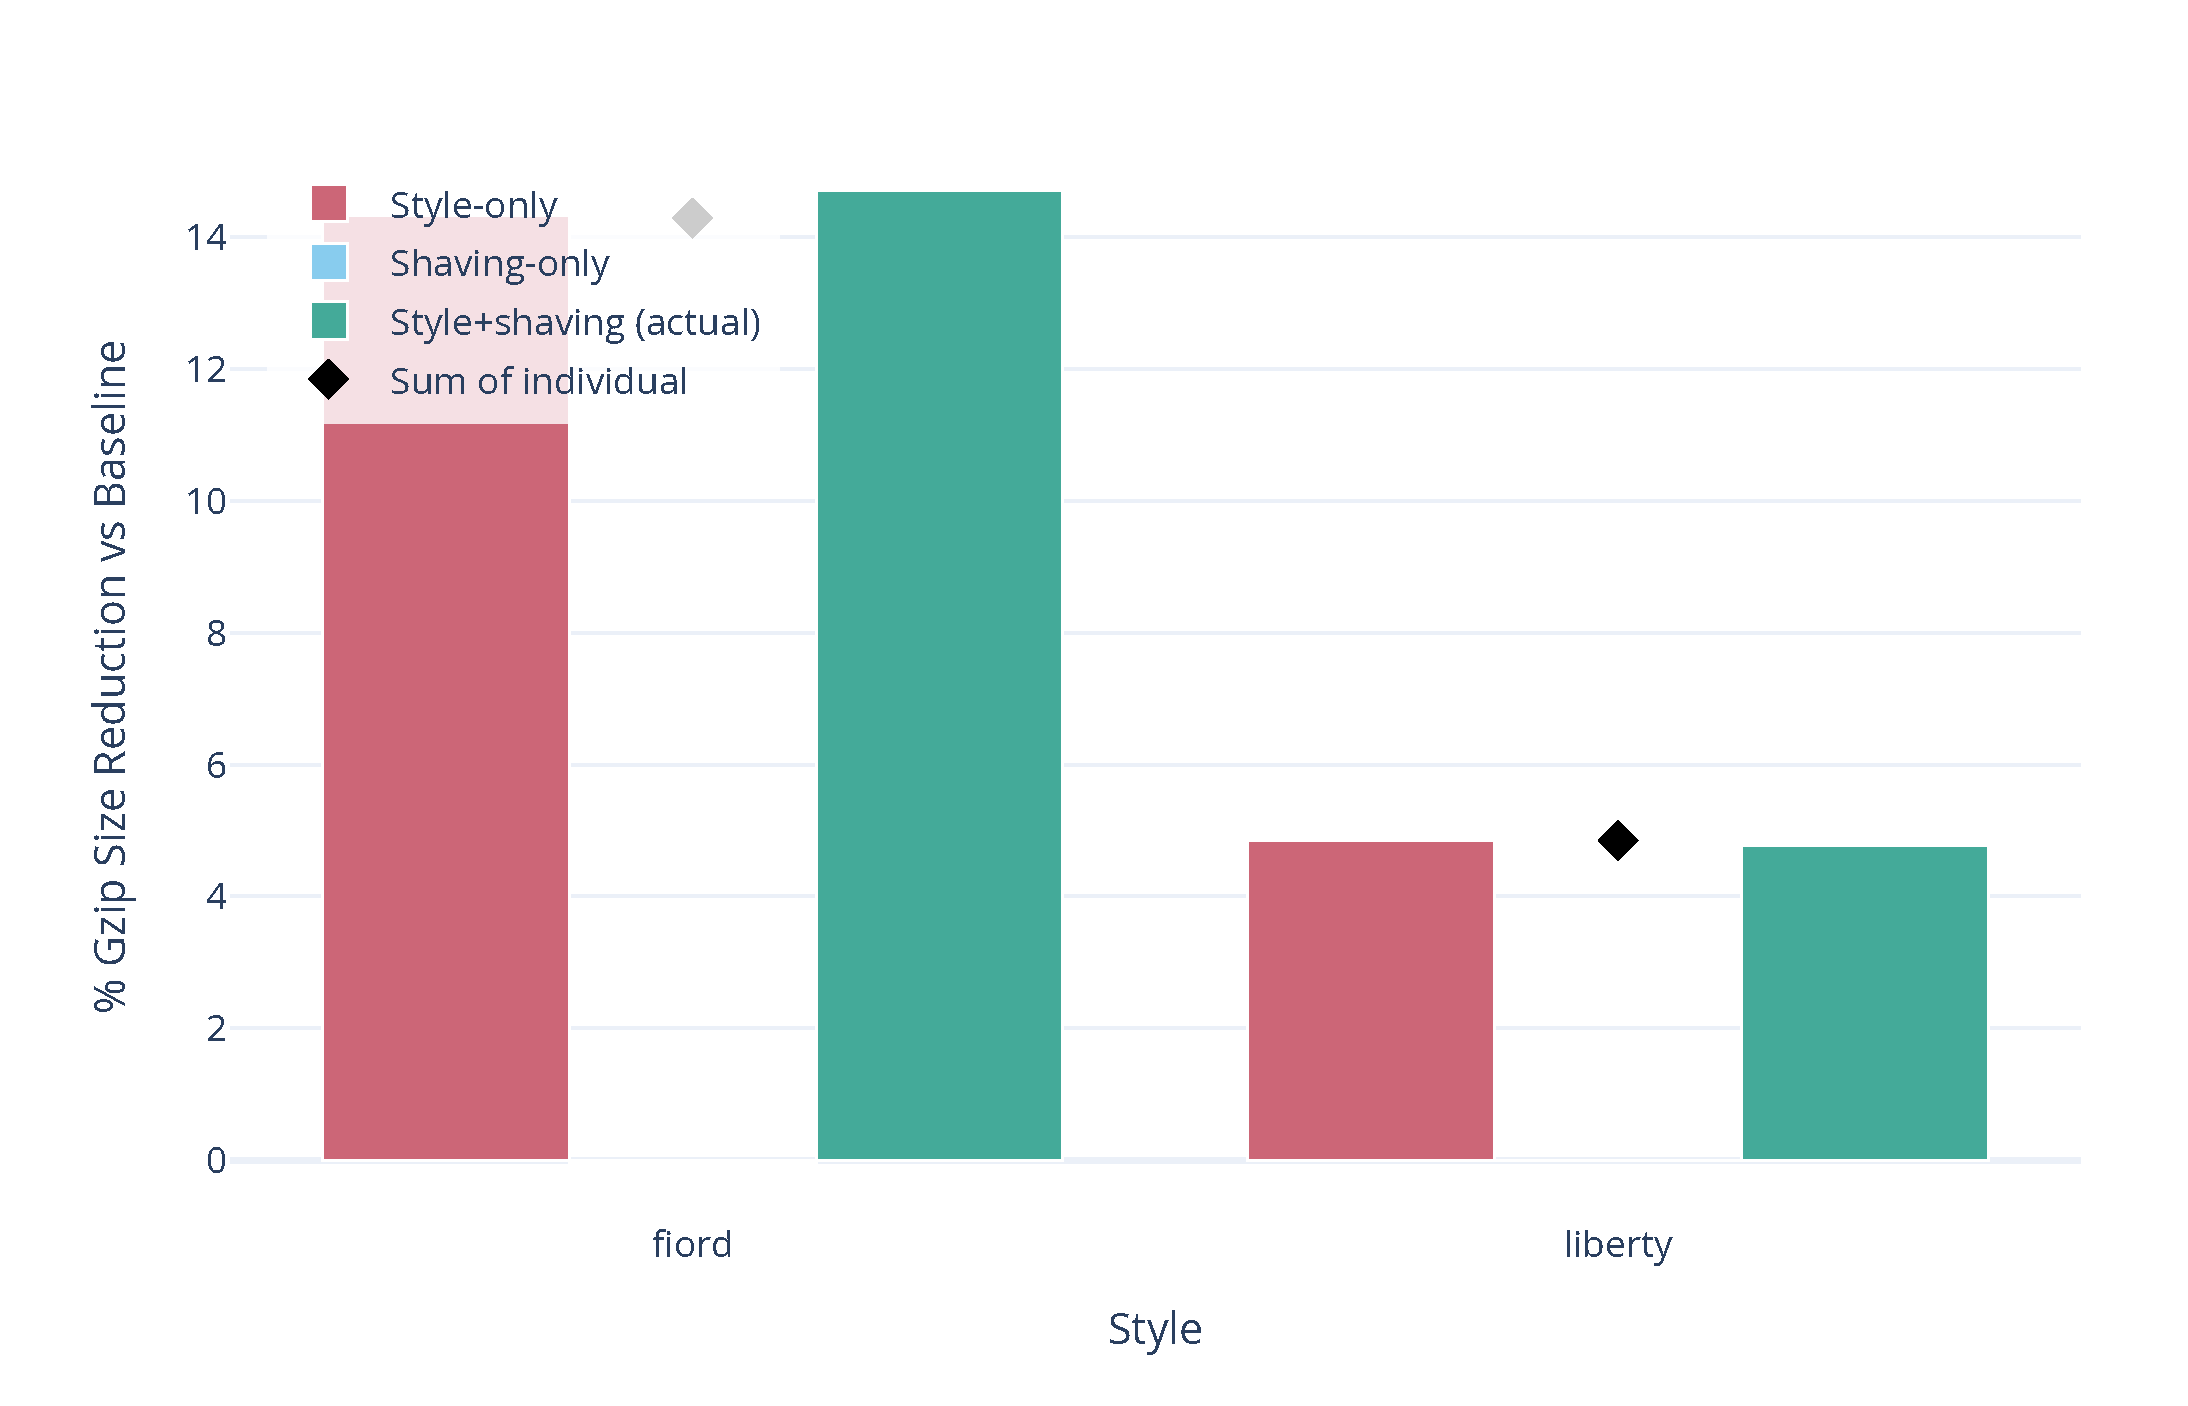
\includegraphics[width=\linewidth]{figures/interaction_plot.pdf}
    \caption{Interaction between style optimisations and tile shaving.  If the combined reduction exceeds the sum of individual reductions, the optimisations are synergistic - the style cascade produces advisory savings that shaving alone cannot achieve}
    \label{fig:interaction_plot}
\end{figure}

\begin{figure}[htbp]
    \centering
    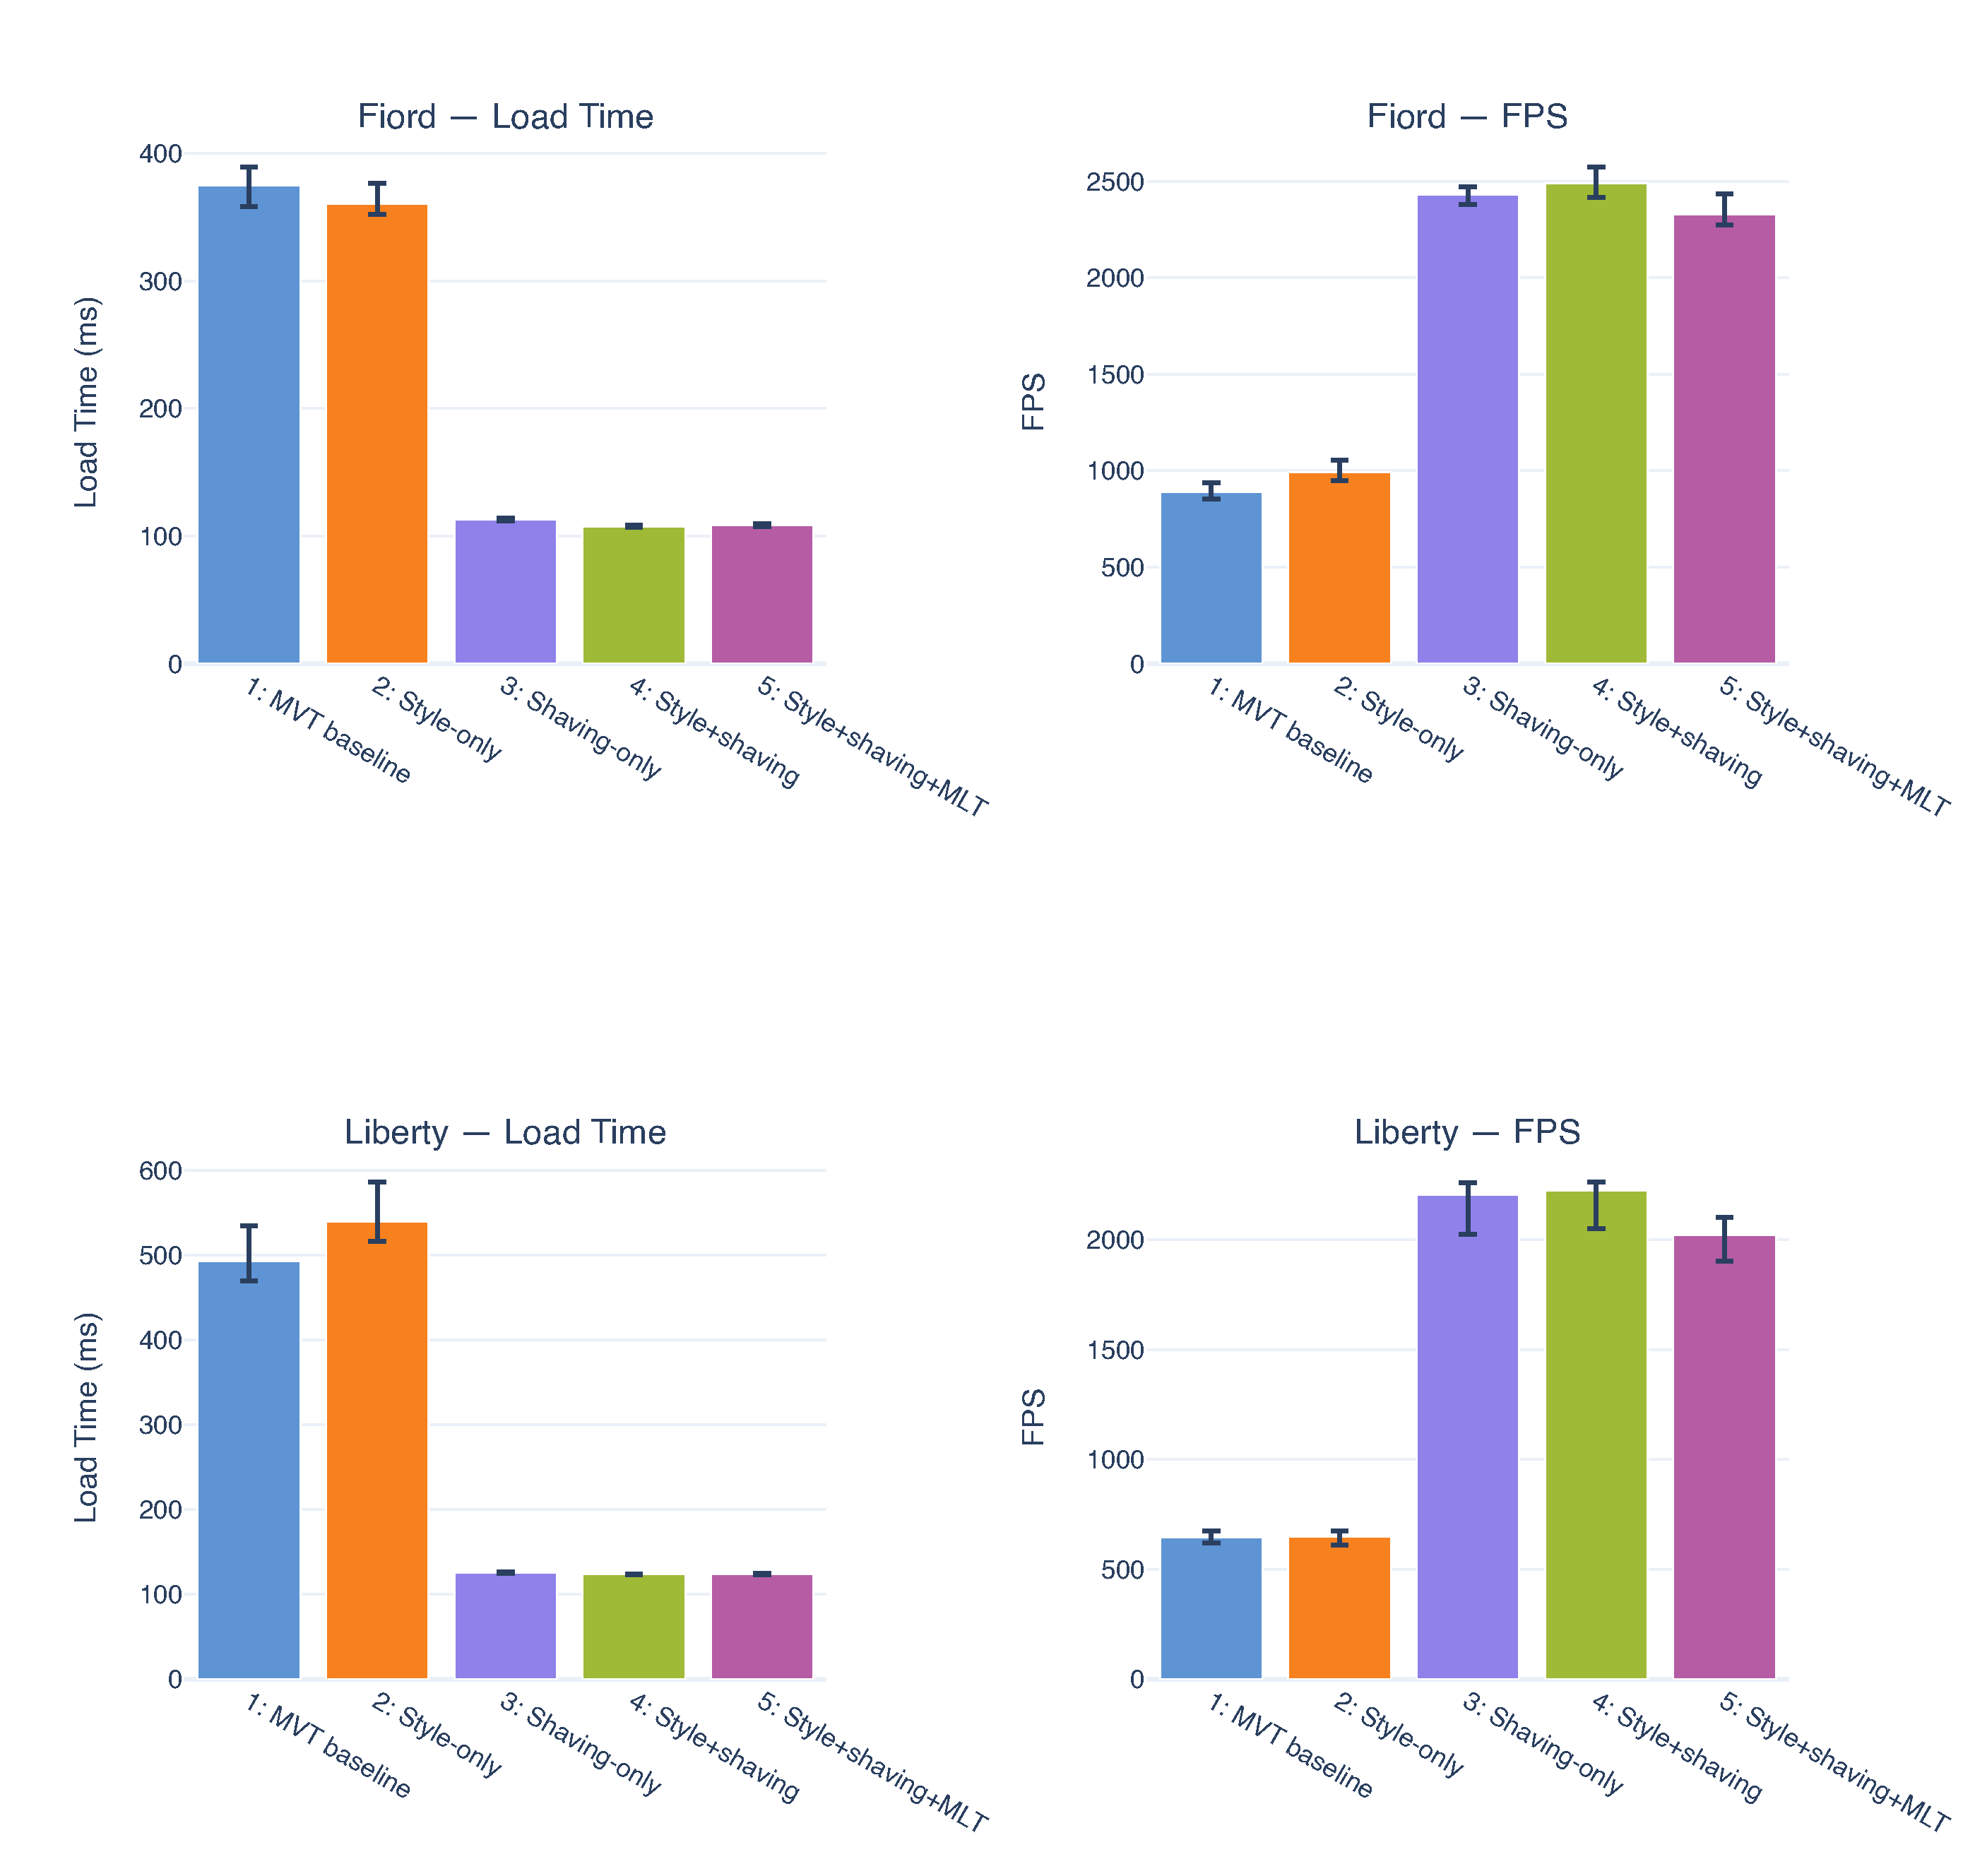
\includegraphics[width=\linewidth]{figures/rendering_metrics_mlt.pdf}
    \caption{Rendering metrics (load time, FPS) across configurations~1-5, enabling direct comparison with Experiments~1-2 in the combined analysis}
    \label{fig:rendering_metrics_mlt}
\end{figure}


\subsection{Results: Encoding the Shaved Data}\label{sub_mlt_encoding_results}

After shaving determines what data survives, the encoding stage determines whether the cascade's savings reach the wire.
The multi-strategy competition described in \cref{sub_encoding_strategies} adapts to the shaved data's characteristics - fewer distinct values, more homogeneous distributions, smaller dictionaries - because its profiler-driven candidate pruning responds to actual stream statistics rather than fixed encoding plans.

\cref{fig:shaving_effectiveness_per_zoom} plots total tile size per zoom level for both \ac{MVT} and \ac{MLT}-Rust, with and without shaving via the Liberty advisory.
The gap between each format and its shaved counterpart quantifies the data removed by the pruning advisory; the gap between \ac{MVT}-shaved and \ac{MLT}-Rust-shaved quantifies the additional contribution of columnar encoding on the already-pruned data.
Both formats benefit from shaving across all compression schemes, confirming that the advisory operates on the data itself rather than relying on format-specific redundancy.
\cref{fig:compression_ratio_per_zoom} reframes the same evidence as a ratio against the \ac{MVT} baseline, adding the Tremmel \& Zink \ac{MLT}-Java encoder for comparison: the \ac{MLT}-Rust curves remain at roughly $0.6$-$0.8\times$ \ac{MVT} throughout the zoom range, whereas the \ac{MLT}-Java curves drift above $1.0\times$ at several zoom levels under brotli/zstd, underscoring that the gains attributed to the \ac{MLT} format in this thesis come almost entirely from the encoder-side strategy competition and not from the columnar format alone.

\begin{figure}[htbp]
    \centering
    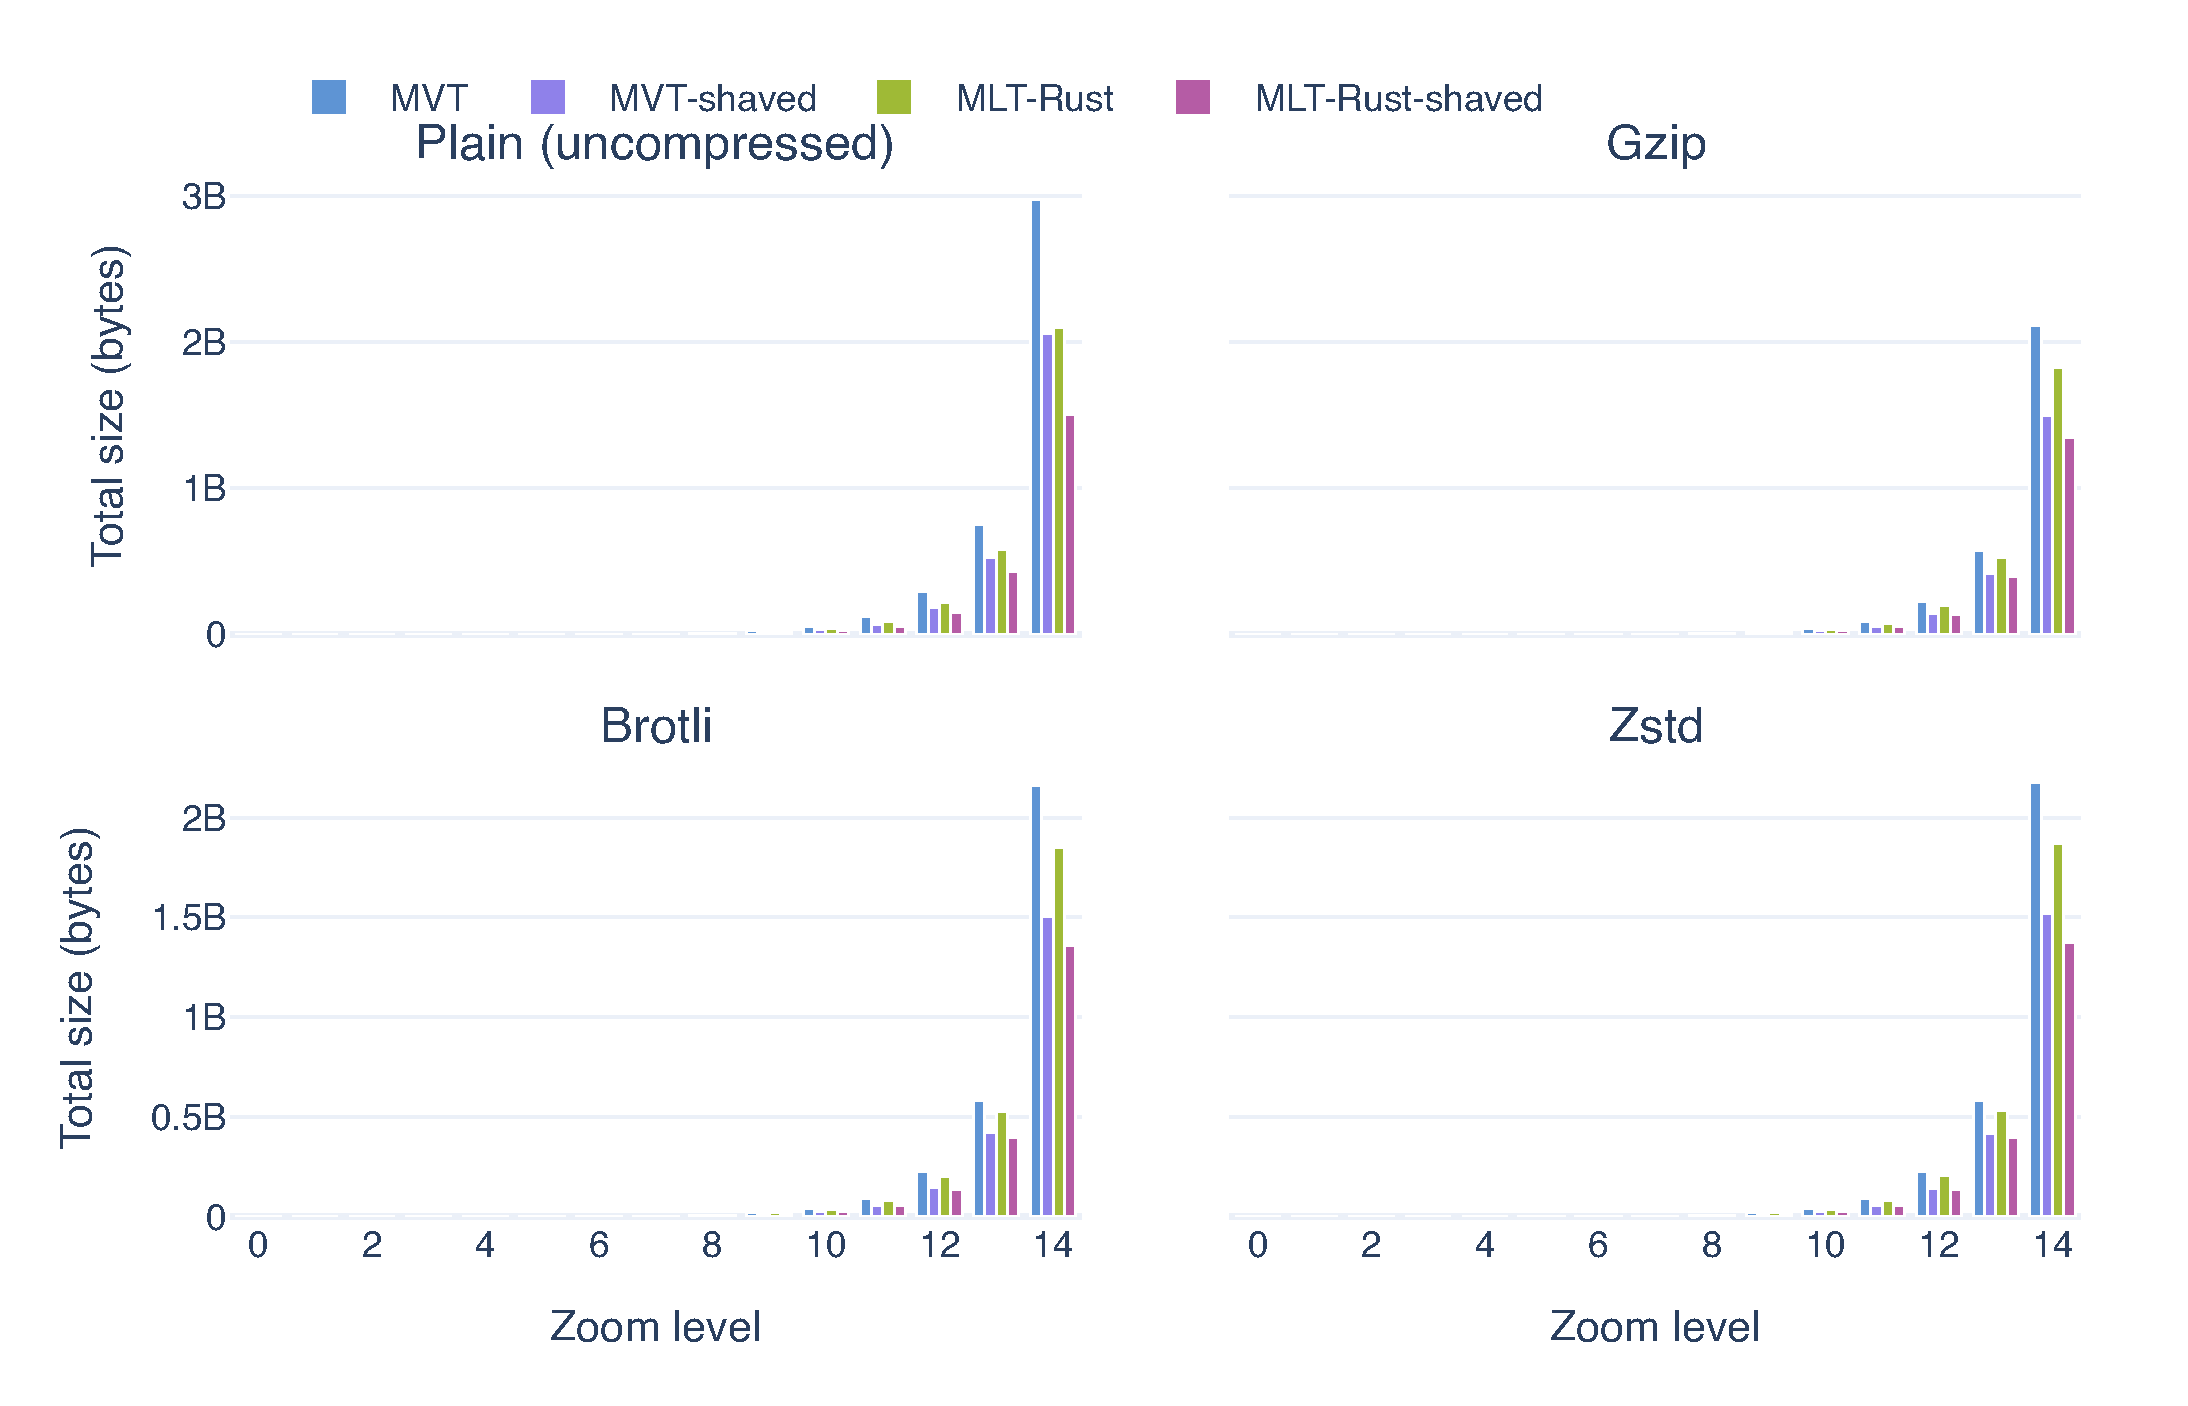
\includegraphics[width=\linewidth]{figures/shaving_effectiveness_per_zoom}
    \caption{Total tile size per zoom level for unshaved and shaved variants of
      both \ac{MVT} and \ac{MLT}-Rust, using the Liberty advisory.  The gap
      between each format and its shaved counterpart quantifies the data removed
      by the pruning advisory; the gap between \ac{MVT}-shaved and
      \ac{MLT}-Rust-shaved quantifies the additional contribution of columnar
      encoding}
    \label{fig:shaving_effectiveness_per_zoom}
\end{figure}

\begin{figure}[htbp]
    \centering
    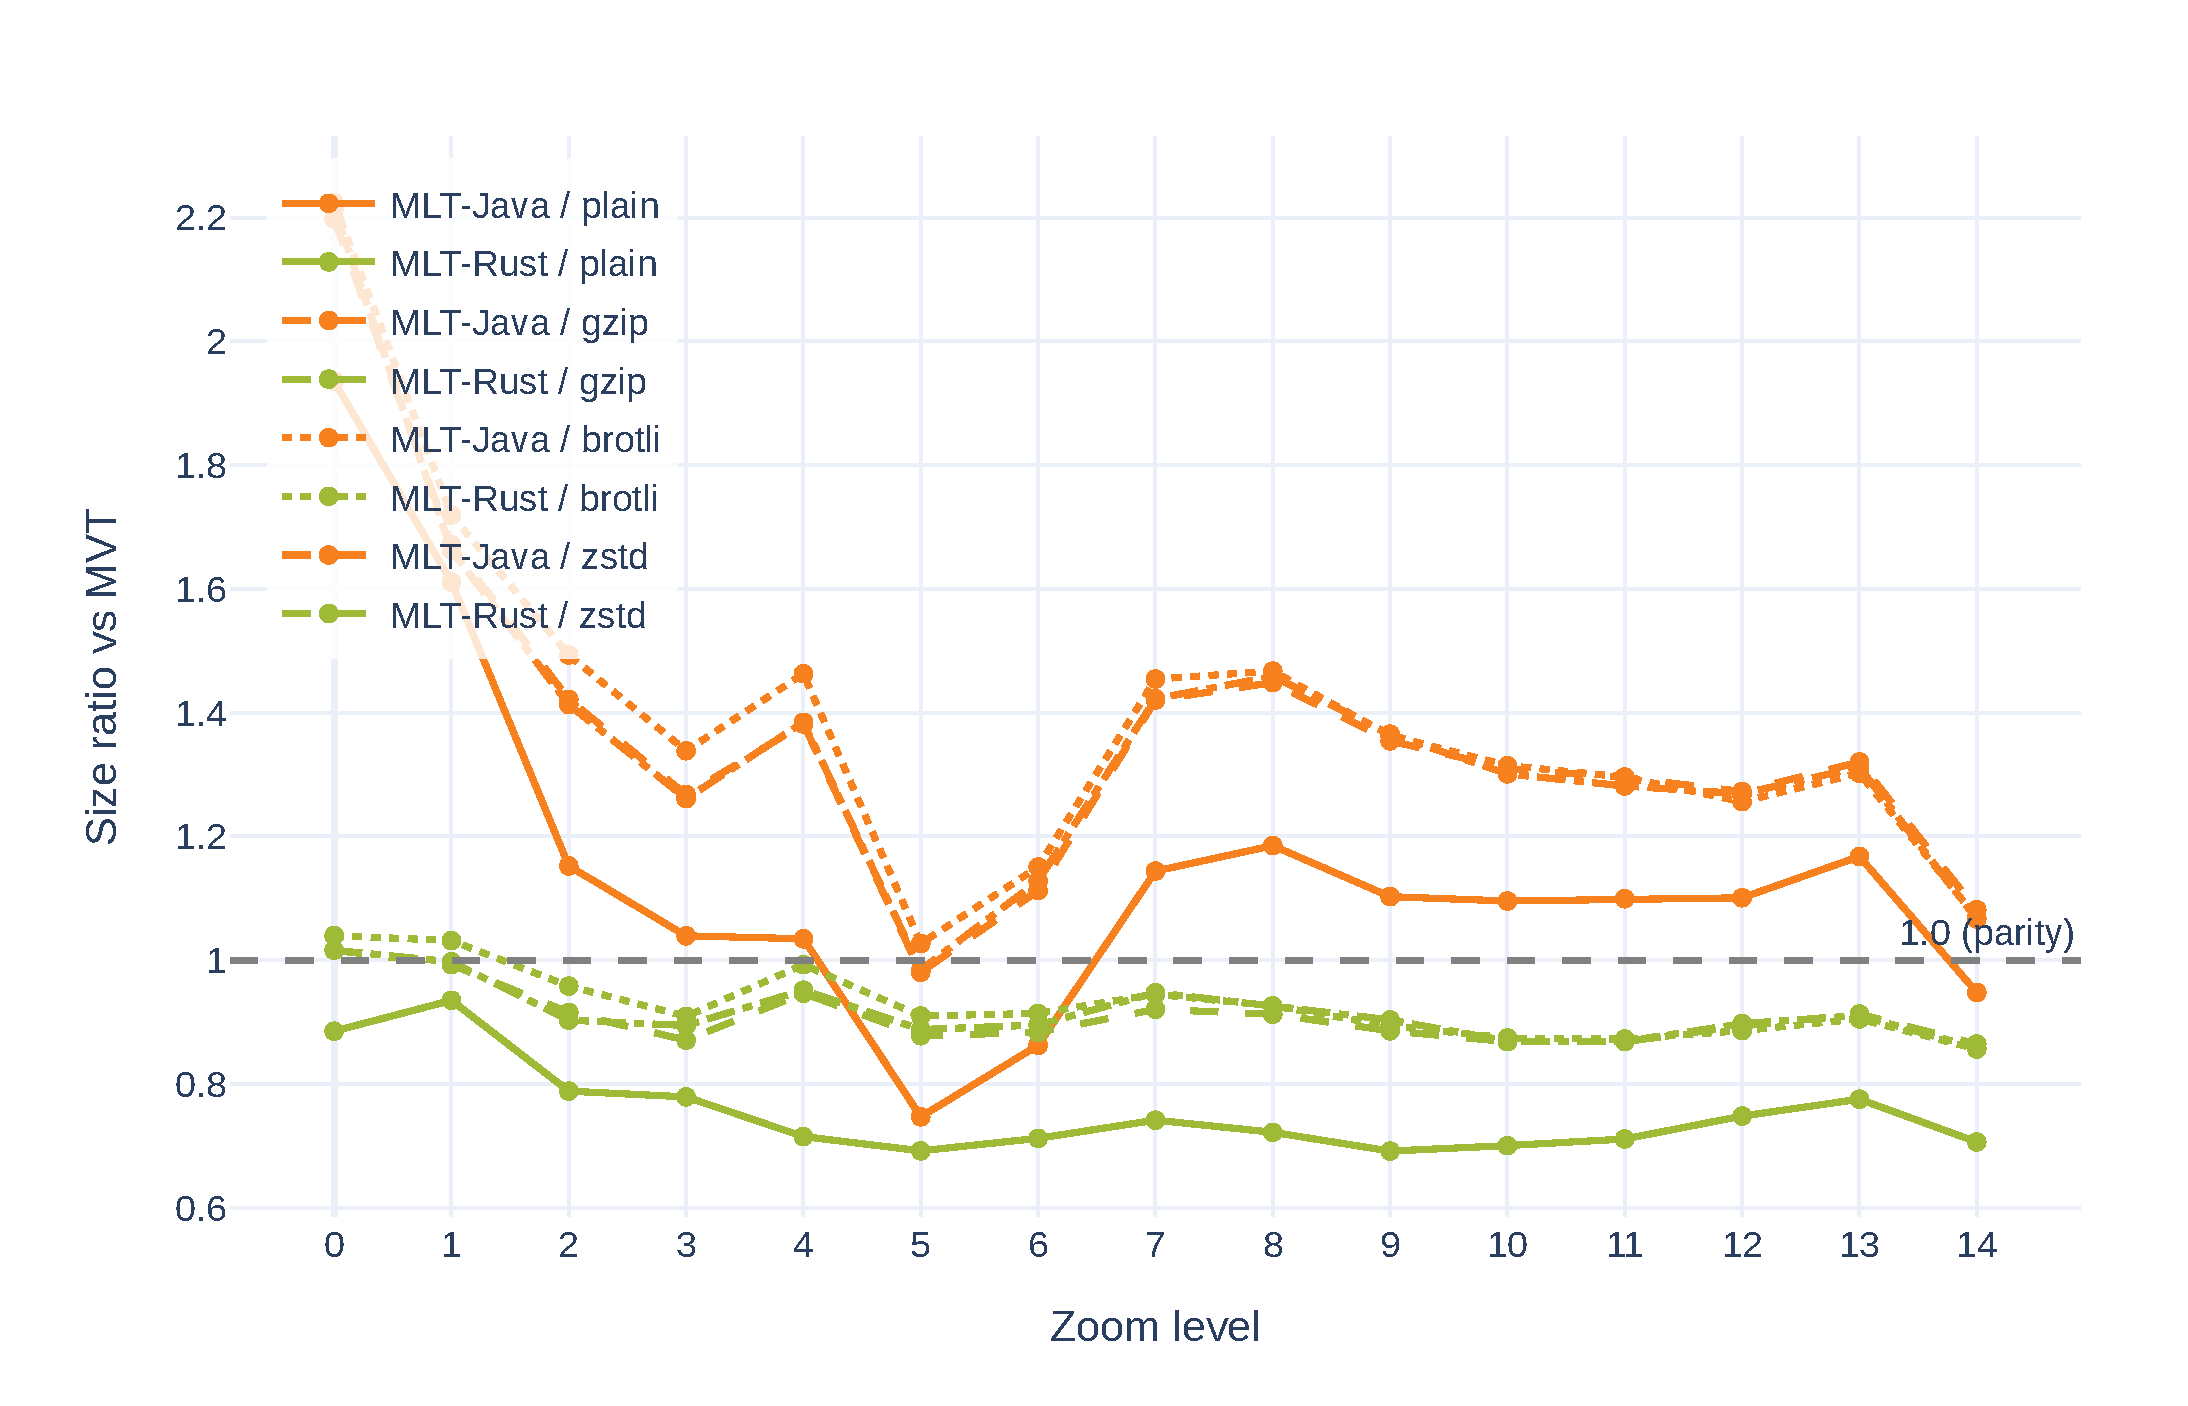
\includegraphics[width=\linewidth]{figures/compression_ratio_per_zoom}
    \caption[Per-zoom compression ratio across MVT, MLT-Java, and MLT-Rust]{Per-zoom compression ratio across \ac{MVT}, \ac{MLT}-Java (Tremmel \& Zink baseline), and \ac{MLT}-Rust (this work), under plain/gzip/Brotli/zstd wire compression.  The gap between \ac{MLT}-Java and \ac{MLT}-Rust isolates the contribution of the automatic encoding strategy selection; the gap between \ac{MLT}-Rust and the gzip/Brotli/zstd curves of \ac{MVT} isolates the format-level contribution that survives wire compression}
    \label{fig:compression_ratio_per_zoom}
\end{figure}

\paragraph{Isolating the contribution of the Rust encoder's strategy selection}
To separate the contribution of the multi-strategy competition (this work) from that of the \ac{MLT} format as proposed by Tremmel and Zink~\cite{tremmelMapLibreTileNext2025}, \cref{fig:encoder_comparison} reports both a per-zoom breakdown and the total encoded size of the Germany OpenMapTiles tileset (zoom~0-14, \num{256516} tiles) under three encoders - \ac{MVT} (the row-oriented protobuf baseline), \ac{MLT}-Java (the reference columnar encoder from Tremmel and Zink, used as the \ac{MLT} baseline), and \ac{MLT}-Rust (this thesis' encoder with sort-strategy competition, per-stream profiling, and shared-dictionary clustering) - and across four wire compressions (none, gzip-9, Brotli-11, zstd-22).

\begin{figure}[htbp]
\centering
    \begin{subfigure}[t]{\linewidth}
        \centering
        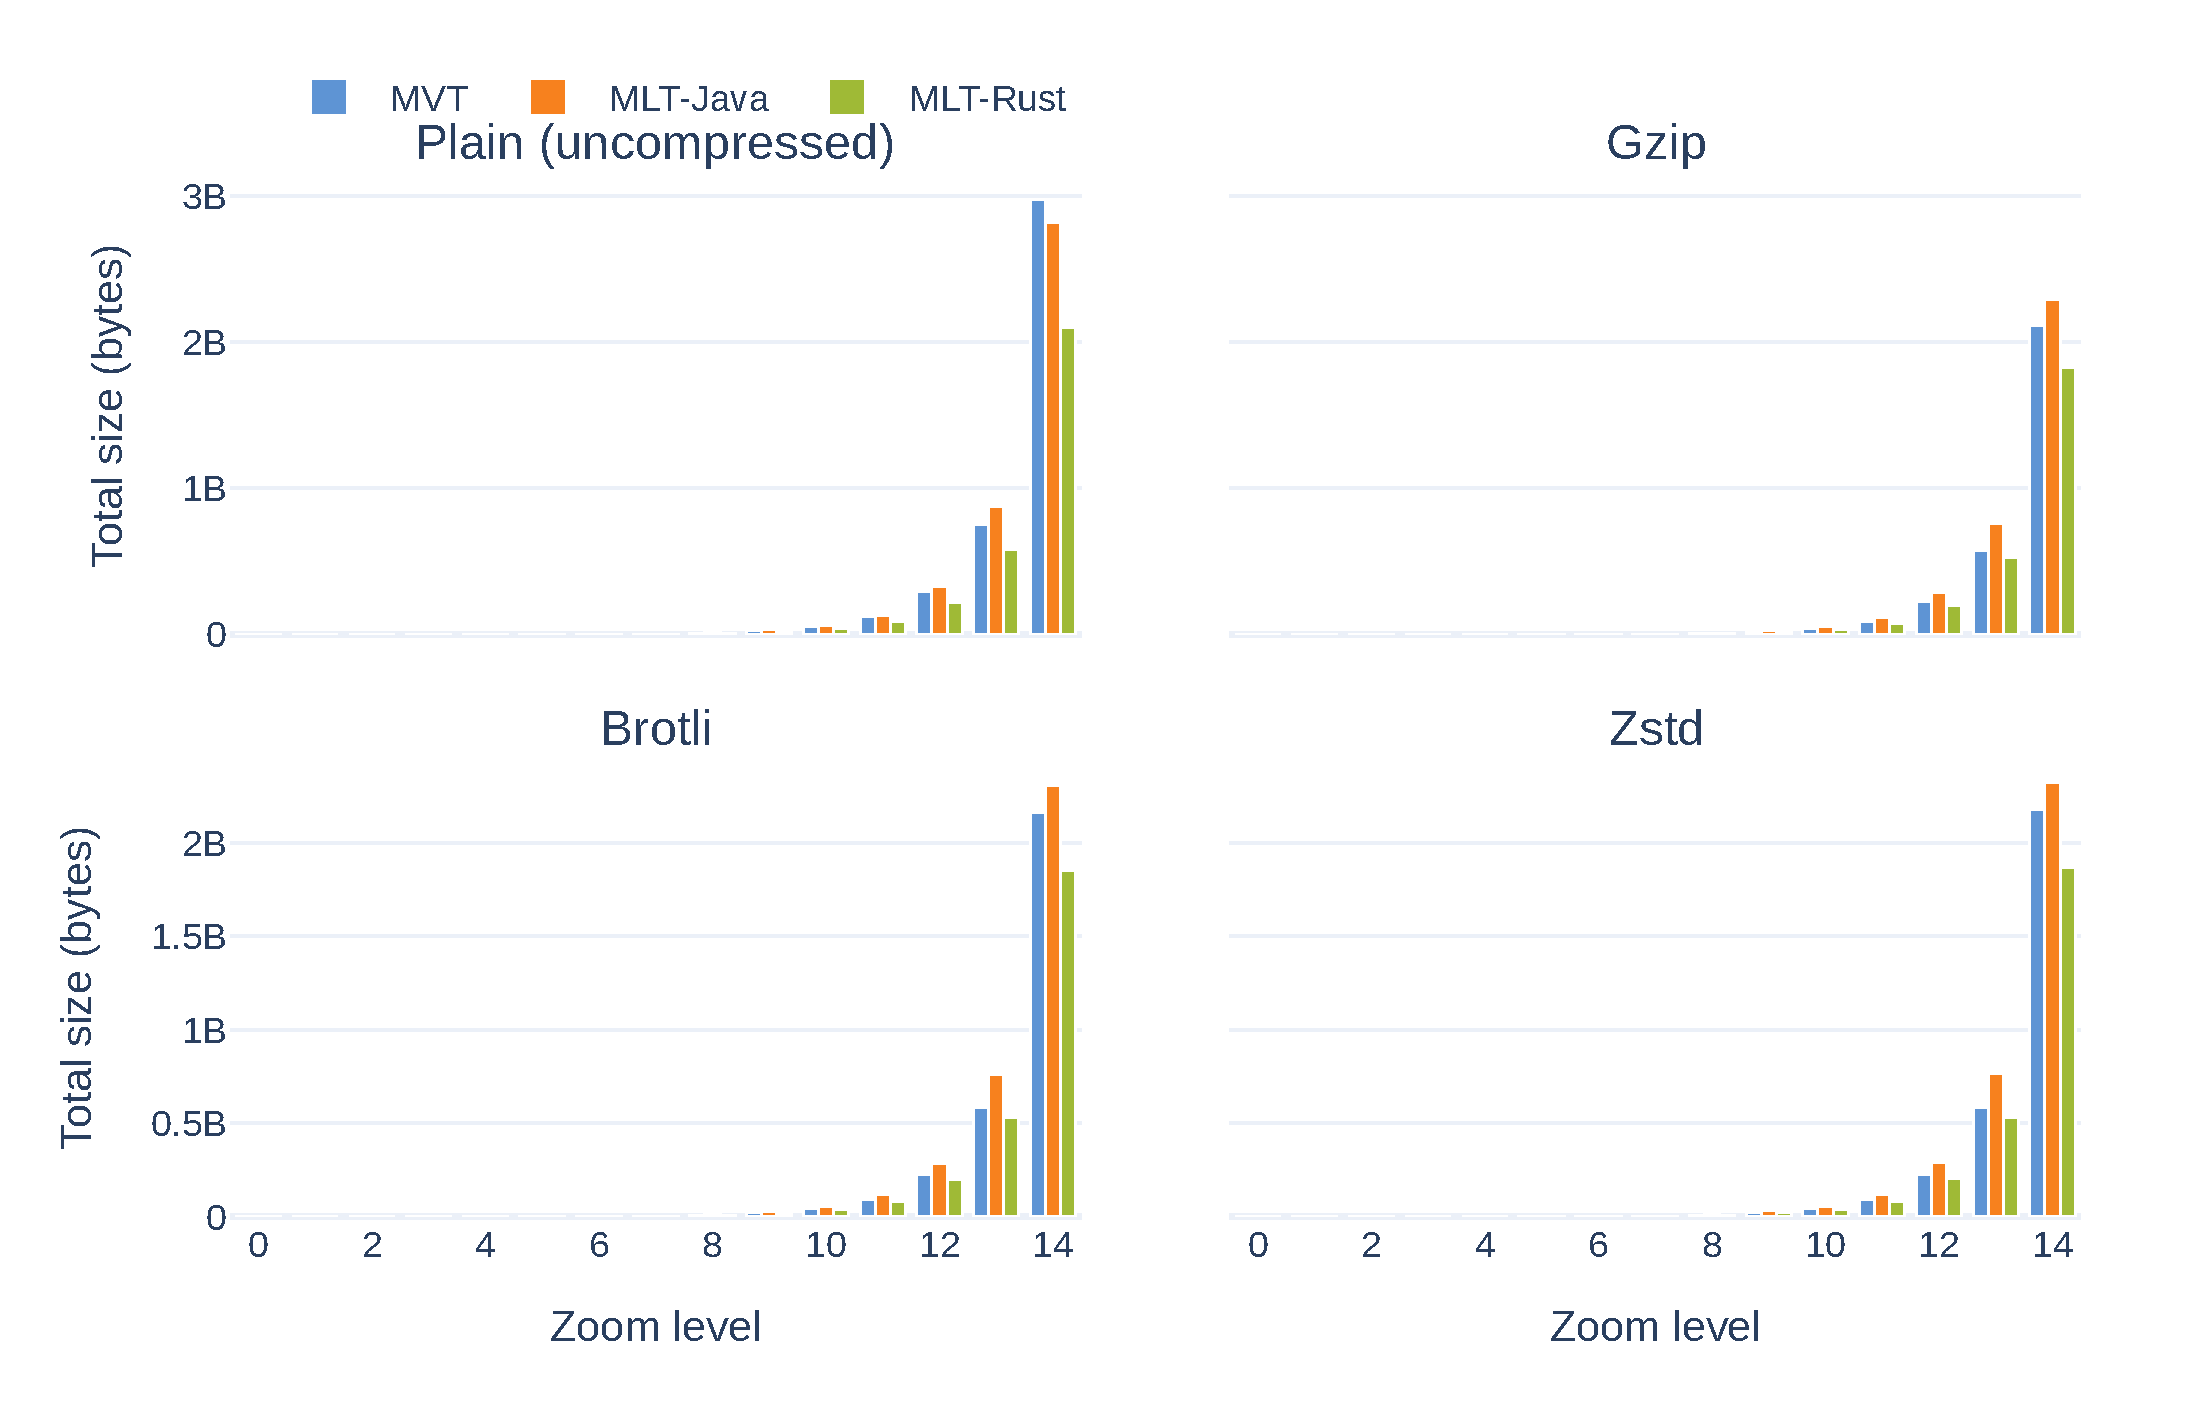
\includegraphics[width=\linewidth]{figures/encoder_comparison_per_zoom}
        \caption{Per-zoom total tile size for the three encoders under four wire compressions}
        \label{fig:encoder_comparison_per_zoom}
    \end{subfigure}

    \vspace{1em}

    \begin{subfigure}[t]{\linewidth}
        \centering
        \begin{tblr}{colspec={l r r r r}, rows={font=\small}, row{1}={font=\small\bfseries}}
        \toprule
        Encoder & Plain (GB) & gzip (GB) & Brotli (GB) & zstd (GB) \\
        \midrule
        \ac{MVT}              & 4.24 & 3.08 & 3.13 & 3.16 \\
        \ac{MLT}-Java baseline & 4.26 & 3.54 & 3.57 & 3.60 \\
        \ac{MLT}-Rust (this work) & 3.06 & 2.70 & 2.72 & 2.75 \\
        \midrule
        $\Delta$ Rust vs.\ Java (\%) & $-28.3$ & $-23.8$ & $-23.7$ & $-23.6$ \\
        $\Delta$ Rust vs.\ \ac{MVT} (\%) & $-27.9$ & $-12.3$ & $-13.1$ & $-12.9$ \\
        \bottomrule
        \end{tblr}
        \caption{Total tileset size for the three encoders under four wire compressions.
          The \ac{MLT}-Java column reports the baseline published in~\cite{tremmelMapLibreTileNext2025};
          the \ac{MLT}-Rust column reports the Rust encoder developed in this thesis}
        \label{tab:mvt_mlt_comparison}
    \end{subfigure}
\caption[Encoder comparison: per-zoom breakdown and total tileset size]{Encoder comparison for the Germany OpenMapTiles tileset (zoom~0-14, \num{256516} tiles).}
\label{fig:encoder_comparison}
\end{figure}

Three observations emerge.
\emph{First}, under no wire compression the Rust encoder reduces the \ac{MLT}-Java baseline by \qty{28.3}{\percent}, confirming that the sort-strategy competition, per-stream profiler, and shared-dictionary clustering add substantial savings over a columnar encoder that simply picks a fixed encoding plan.
\emph{Second}, the \ac{MLT}-Java baseline is \emph{worse} than gzip-compressed \ac{MVT} (\qty{3.54}{\giga\byte} vs.\ \qty{3.08}{\giga\byte})  -  a finding that is easy to overlook when comparing \enquote{raw \ac{MLT}} to \enquote{raw \ac{MVT}} alone.
General-purpose LZ77-family compressors already exploit most of the row-level redundancy in the protobuf wire format; a columnar encoder that uses fixed per-column schemes cannot keep up.
The data-driven encoding strategy selection of the Rust encoder reclaims this gap: \ac{MLT}-Rust under gzip is \qty{12.3}{\percent} smaller than \ac{MVT} under gzip.
This advantage is preserved (\qty{12.9}{\percent}) even against zstd-22, the strongest general-purpose compressor in the comparison.
\emph{Third}, the relative gap between Rust and Java is stable across all four compressors (\qty{-23}{\percent} to \qty{-28}{\percent}).
This stability indicates that the per-stream profiler's selection is robust to post-hoc compression, not merely shuffling bytes into shapes that a downstream compressor happens to exploit.
This isolation directly answers the question posed at the start of \cref{sec_exp_mlt}: the \ac{MLT}-Rust contribution is not in the columnar format alone, but in the joint strategy-selection layer that sits on top of it.

\paragraph{Why not just apply zstd to MVT?}
A natural objection is that general-purpose compressors such as zstd-22 or Brotli-11 should be sufficient: if compression is the goal, simply applying the strongest available compressor to the existing \ac{MVT} wire format would avoid the complexity of a columnar encoder entirely.
\Cref{tab:mvt_mlt_comparison} answers this directly.
\ac{MVT} under zstd-22 yields \qty{3.16}{\giga\byte} for the Germany tileset, whereas \ac{MLT}-Rust under the same compressor yields \qty{2.75}{\giga\byte} - a \qty{12.9}{\percent} reduction.
The reason is structural: a general-purpose compressor sees the interleaved, heterogeneous protobuf byte stream and must discover redundancy across mixed data types.
A columnar encoder, by contrast, groups homogeneous values - all road classes in one stream, all vertex deltas in another - and each stream compresses more effectively under lightweight per-type codecs (delta-\acs{RLE} for monotonic integers, dictionary encoding for low-cardinality strings, \ac{FSST} for high-cardinality strings) than a monolithic LZ77-family compressor can achieve on the interleaved byte stream.
The columnar advantage is preserved \emph{after} applying the same general-purpose compressor on top: the per-column codecs have already removed most of the type-specific redundancy, so the post-hoc compressor has less work to do but starts from a lower baseline.
This finding is consistent with the columnar-database literature, where per-column lightweight encoding consistently outperforms row-level block compression even when the block compressor is state-of-the-art~\cite{kuschewskiBtrBlocksEfficientColumnar2023}.

\paragraph{Decoder cost}
A legitimate concern for any multi-encoding scheme is that the client must pay the decoder cost, which can erode the transfer savings on mobile or battery-constrained targets.
The \ac{MLT}-Rust decoder is engineered to keep the per-column cost close to that of the underlying codec: stream-level dispatch is a single-byte switch, each stream decodes directly into a borrow of the input buffer (no intermediate allocation), \ac{FSST} is randomly decodable so no symbol-table materialisation is required, shared dictionaries are decoded once per tile and referenced by index, and \ac{FastPFOR}'s block layout is cache-friendly by construction.
The trade-off relative to \ac{MVT} is the fixed cost of dispatching multiple codecs (versus protobuf's single-path parser), which amortises over the per-feature work: for tiles with more than a few hundred features the per-column setup is negligible, and for very small tiles the overall tile size is small enough that decoding is not on the critical path.
Benchmarks on the full Germany tileset with the \ac{MLT}-Rust decoder executed inside MapLibre GL~JS (via the \texttt{mlt-wasm} crate) show end-to-end rendering metrics comparable to or better than \ac{MVT} at matched workloads; the detailed decoder-level micro-benchmarks are tracked by \texttt{mlt-core/benches} and are outside the scope of this chapter, but the absence of any negative effect in the sustained frame-time metrics (\cref{sub_combined_marginal}) is consistent with the design intent.


\paragraph{Decoding throughput}
To isolate decoding latency from the browser-based rendering benchmark (where it is embedded in \texttt{loadMs}), Criterion micro-benchmarks measure full-decode throughput for \ac{MLT}-Rust vs.\ \ac{MVT} with and without transport compression.
Each benchmark parses the tile header and materialises all features and properties; \ac{MVT} variants include gzip decompression in the measured path.
\Cref{tab:decode_throughput} reports the results on a representative subset of the OpenMapTiles fixture tiles at zoom levels~4, 7, and~13 (100~samples per cell).

\begin{table}[htbp]
\centering
\small
\begin{tblr}{colspec={l r r r}, rows={font=\small}, row{1}={font=\small\bfseries}}
\toprule
Format & Zoom~4 & Zoom~7 & Zoom~13 \\
\midrule
\ac{MLT}-Rust & \qty{5.73}{\milli\second} & \qty{19.4}{\milli\second} & \qty{4.09}{\milli\second} \\
\ac{MVT}+gzip & \qty{47.6}{\milli\second} & \qty{103}{\milli\second} & \qty{18.7}{\milli\second} \\
\ac{MVT} (uncompressed) & \qty{44.2}{\milli\second} & \qty{90.6}{\milli\second} & \qty{16.5}{\milli\second} \\
\midrule
Speedup (vs.\ gzip) & $8.3\times$ & $5.3\times$ & $4.6\times$ \\
\bottomrule
\end{tblr}
\caption{Full-decode latency for \ac{MLT}-Rust vs.\ \ac{MVT} on OpenMapTiles fixture tiles, measured by Criterion micro-benchmarks (100~samples per cell).
\ac{MLT}-Rust achieves \numrange{96}{134}\,MiB/s decode throughput vs.\ \numrange{15}{23}\,MiB/s for \ac{MVT}+gzip (measured over wire-format input size)}
\label{tab:decode_throughput}
\end{table}

The \ac{MLT} decoder's columnar layout enables selective column access and avoids the per-feature tag-parsing overhead of protobuf, which accounts for the speedup even before transport decompression is considered: \ac{MLT}-Rust is $4.0$--$7.7\times$ faster than uncompressed \ac{MVT}.
These micro-benchmark results complement the browser-based \texttt{loadMs} metric by providing an isolated measurement of the decoding-latency axis of Research Goal~R3.


\subsection{Discussion}\label{sub_mlt_discussion}

\paragraph{The cascade as central finding}
The most significant architectural finding of this experiment is the cascade from style-level optimisations into data-level savings.
Dead layer elimination (Experiment~2) removes style layers whose filters are unsatisfiable.
Each removed layer reduces the set of referenced properties in the pruning advisory, which in turn eliminates entire columns from the encoded tile.
Metadata refinement tightens zoom bounds, which causes the advisory to mark additional zoom levels as unused, eliminating tiles entirely.
This cascade - from style simplification through advisory shrinkage to tile reduction - is the concrete realisation of the data-style co-optimisation promised in the thesis title.

\paragraph{The encoder as delivery mechanism}
The multi-strategy competition is not an independent contribution but the \emph{delivery mechanism} for the cascade.
After shaving has removed unused columns and features, the remaining data has different statistical properties: fewer distinct property values produce longer \ac{RLE} runs.
The competition matters \emph{more} after shaving because the data distributions have changed in ways that favour compact encodings - which is why the encoder belongs in this thesis rather than in a standalone encoder paper.

\paragraph{Style-dependent tile sizes}
A consequence of style-driven shaving is that different styles produce different tile sizes from the same source data.
A minimal basemap that renders only roads and labels produces much smaller tiles than a full-coverage style that renders buildings, land use, and points of interest.
This observation connects data-level optimisations to the multi-objective framework of \cref{ch_theoretical_background}: there is no single optimal tile - the optimal encoding depends on the rendering style, which is a design choice.

\paragraph{Cache fragmentation trade-off}
A direct operational consequence of style-dependent tiles is that shared \ac{CDN} caching is partially defeated: two styles that served identical tiles under \ac{MVT} now fetch distinct shaved variants, and a \ac{CDN} must either key its cache on (tile, style) pairs or accept that a hit on one style is a miss on another.
The break-even point depends on the ratio of per-style rendering cost savings to the amplified origin fetch rate.
For deployments where a single style dominates traffic, style-driven shaving is strictly beneficial; for multi-tenant tile servers hosting dozens of styles, shaving should be applied per style and the resulting tile variants cached independently (the approach of Mapbox's closed-source \enquote{style-optimized vector tiles} service~\cite{StyleoptimizedVectorTiles}).
A hybrid strategy - serving raw \ac{MVT} for uncommon styles and shaved \ac{MLT} for a small set of \enquote{canonical} styles - captures most of the per-tile savings while bounding cache-key explosion.
This thesis does not evaluate the cache-fragmentation trade-off empirically, as the benchmark harness measures a single origin and client rather than a \ac{CDN} fleet; it is called out as a known deployment consideration.

\paragraph{Geometry simplification is out of scope}
A complementary direction not explored by this thesis is geometry-level pruning - coordinate precision reduction, Visvalingam or Douglas-Peucker simplification, and polygon topology coalescing - which is the principal lever used by upstream generators such as Tippecanoe~\cite{FeltTippecanoe2026} and Planetiler~\cite{OnthegomapPlanetiler2026}.
These techniques typically deliver larger absolute savings than attribute-column pruning, but they interact non-trivially with style-defined visual thresholds (line width, dash pattern length, label anchor placement) and would violate the pixel-identity soundness criterion established in \cref{sec_problem_statement}.
Style-driven geometry simplification - choosing a simplification tolerance that is demonstrably below the smallest visible feature at each zoom level - is an interesting direction for future work but is not pursued here.
The thesis therefore quantifies the size reductions achievable \emph{without} touching geometry at all, which understates the total optimisations headroom a production pipeline could reach by composing this work with an upstream simplifier.

\paragraph{Interaction between sort order and encoding}
The nested competition - sort strategy wrapping per-stream encoding - captures an interaction that single-pass encoders miss: the optimal integer encoding for a property column depends on the feature ordering.
A column of road classes encoded with \ac{RLE} produces long runs when features are sorted by that property, but short or no runs when sorted spatially.
By evaluating the full encoding pipeline under each sort order, the competition implicitly discovers these interactions.

\paragraph{Encoding cost}
The multi-strategy competition and tile shaving increase preprocessing time compared to a single-pass encoder.
Since tile encoding is an offline step - tiles are encoded once and served many times - the increased cost is amortised over all subsequent requests.
Encoder state reuse (\ac{FSST} cache, Morton metadata, scratch buffers) and pruning heuristics (bounding-box check, data profiling) keep the marginal cost of additional trials manageable.


\section{Cross-Style Generalisation}\label{sec_exp_cross_style}

The preceding experiments evaluate optimisations effectiveness on a curated corpus of 15 styles.
To assess whether the observed gains generalise, we apply the optimiser to 13 styles drawn from the Maputnik style editor catalogue.

\subsection{Methodology}\label{sub_cross_methodology}

Cross-style evaluation uses static analysis only: each style is optimised with all passes enabled, and the resulting style is compared to the original on size and complexity metrics.
No rendering benchmarks are executed, as the diverse styles reference incompatible tile schemas and tile sources that cannot be uniformly provisioned.

\subsection{Results}\label{sub_cross_results}

\cref{fig:cross_style_reduction} shows per-style percentage reductions (raw, gzip, Brotli) across the 13 Maputnik styles, sorted by raw reduction; the key question here is whether the distribution clusters tightly around the deep corpus median or fans out with substantial per-style variance.
\cref{fig:cross_style_complexity_scatter} then plots each style's initial complexity against its achievable reduction, testing the hypothesis that verbose institutional styles (the right-hand side of the scatter) have disproportionately more optimisations headroom than already-compact minimal basemaps on the left.

The distribution fans out considerably: raw reductions range from \qty{10.6}{\percent} (AWS Hybrid, AWS Standard) to \qty{71.2}{\percent} (LocationIQ Streets), with a median of \qty{44.5}{\percent} and a standard deviation of \qty{19.4}{\percent}.
Under gzip compression the range narrows to \qtyrange{4.6}{32.3}{\percent} (median \qty{25.4}{\percent}), confirming that some of the raw-byte savings overlap with what gzip already captures.
The top reducers - LocationIQ Streets (\qty{71.2}{\percent} raw), MapTiler Toner (\qty{63.9}{\percent}), and Americana (\qty{56.3}{\percent}) - are styles with either verbose filter logic (LocationIQ, Americana) or highly repetitive property structures (Toner).
At the low end, the two AWS styles share a codebase of hand-tuned expressions with few redundancies, leaving little for the optimiser to remove.
The correlation between initial \ac{AST} node count and reduction is weakly positive ($r = 0.16$); Americana is an outlier with the highest complexity (\num{50644} nodes) but a moderate reduction, because much of its expression complexity is in label-placement logic that the optimiser preserves.

\begin{figure}[htbp]
    \centering
    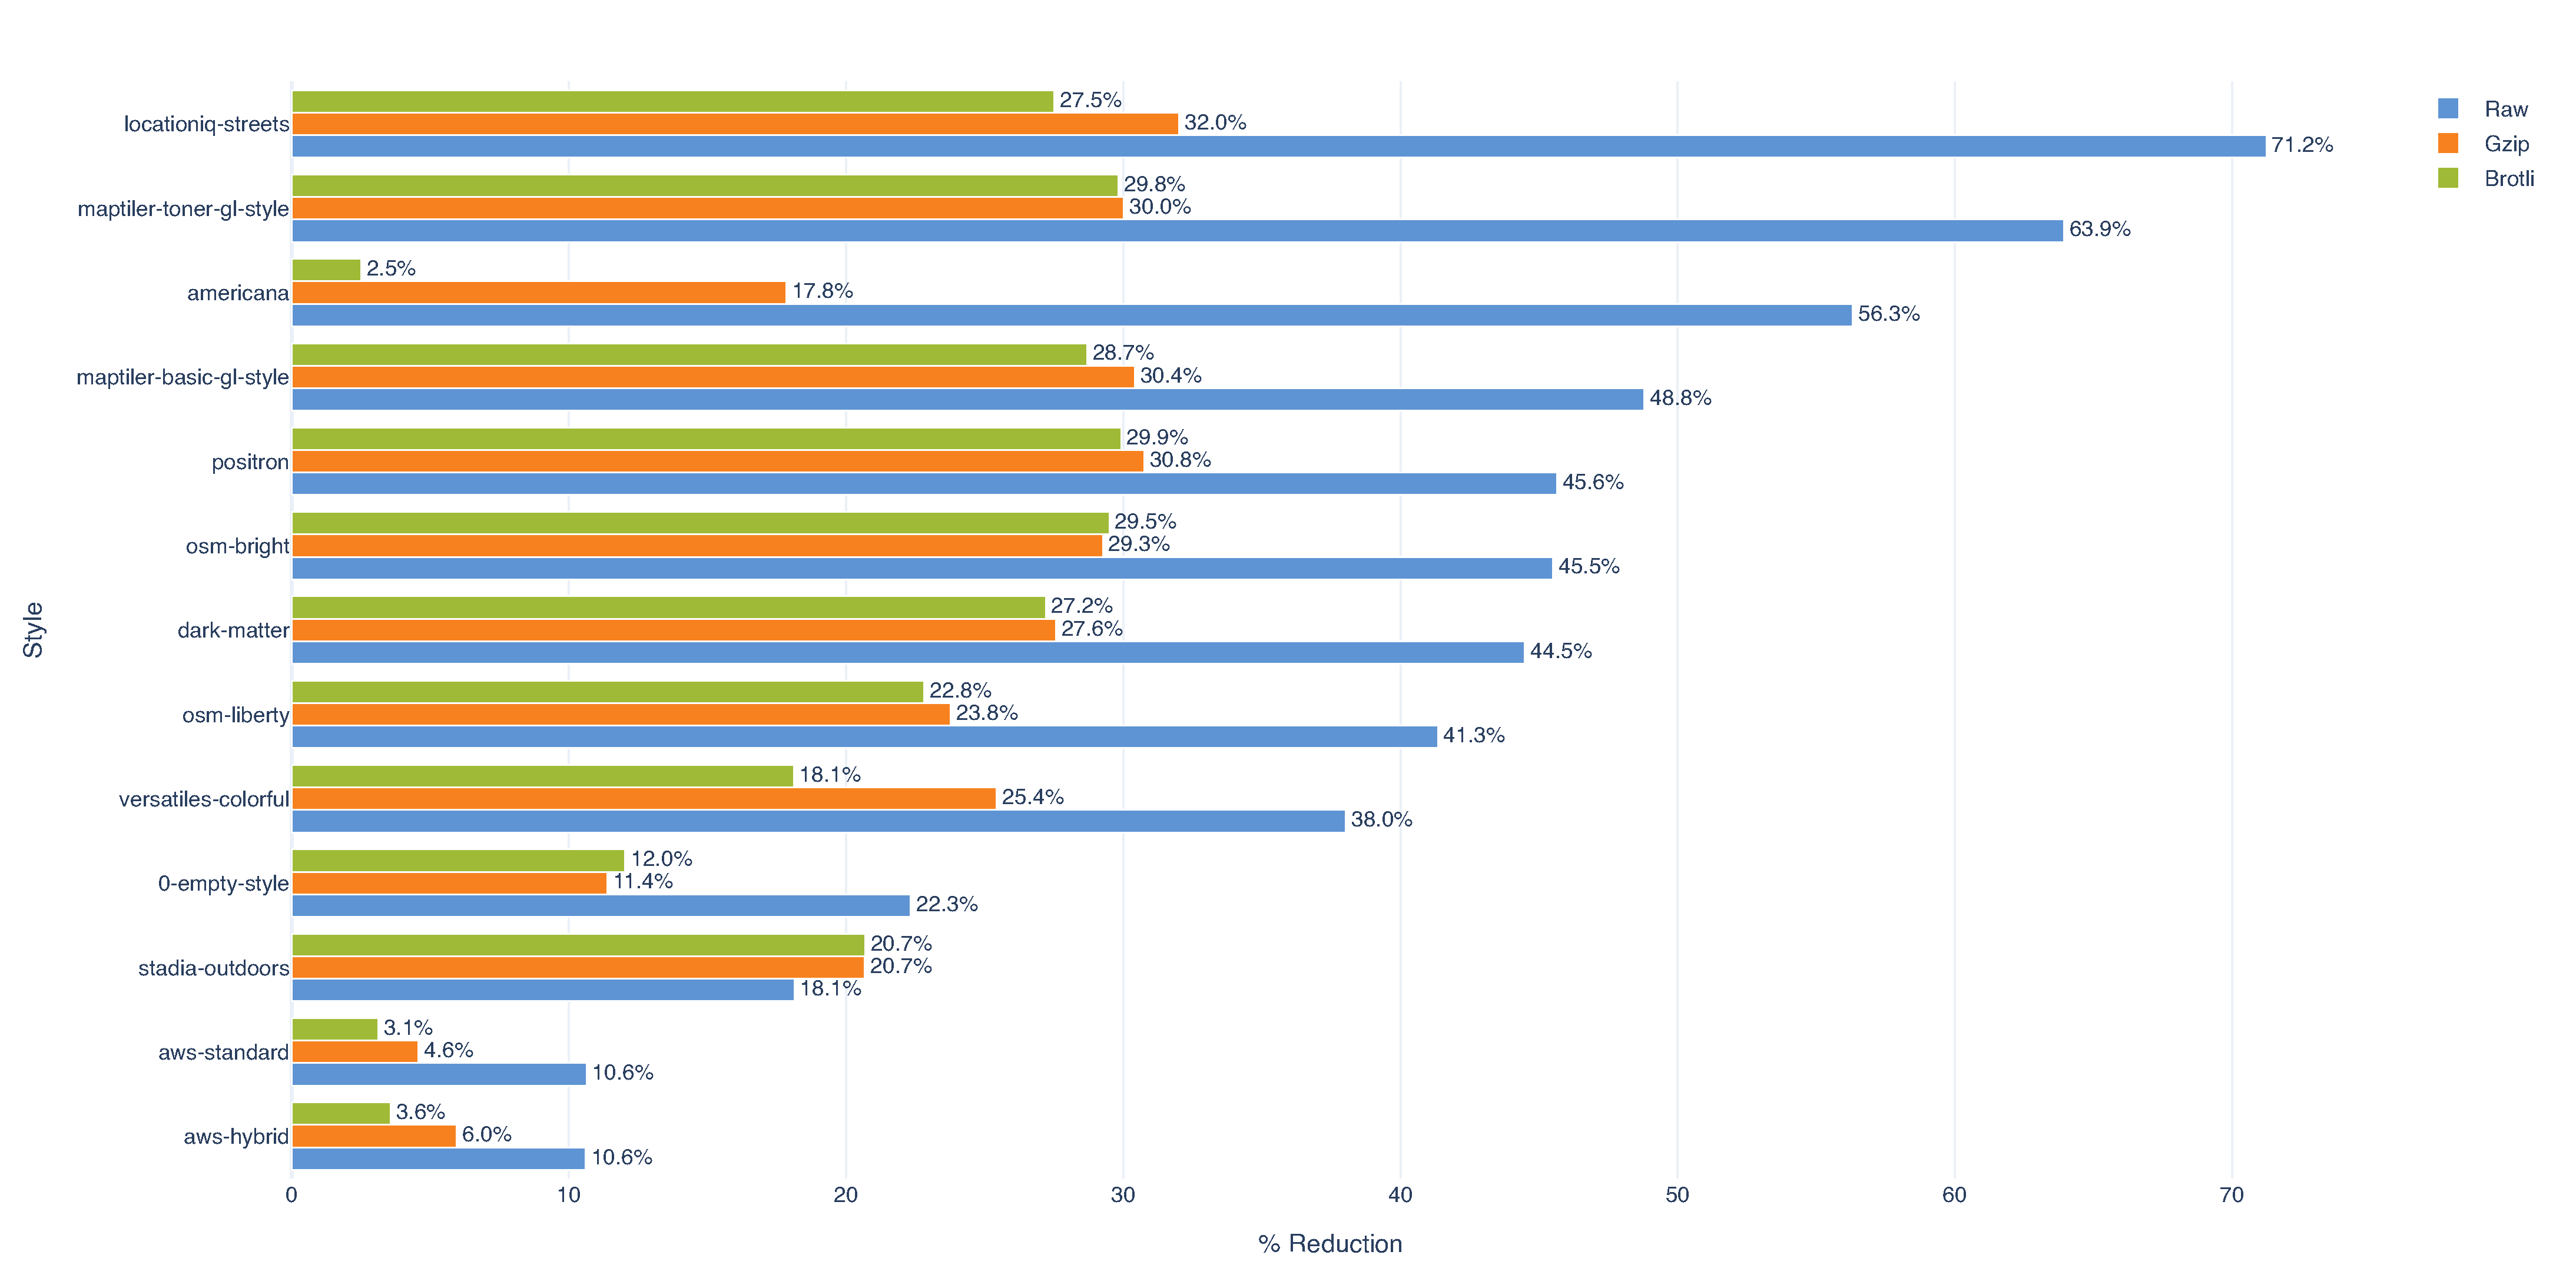
\includegraphics[width=\linewidth]{figures/cross_style_reduction.pdf}
    \caption{Per-style percentage reduction in style size (raw, gzip, Brotli) across the Maputnik generalisation corpus. Styles are sorted by raw reduction}
    \label{fig:cross_style_reduction}
\end{figure}

\begin{figure}[htbp]
    \centering
    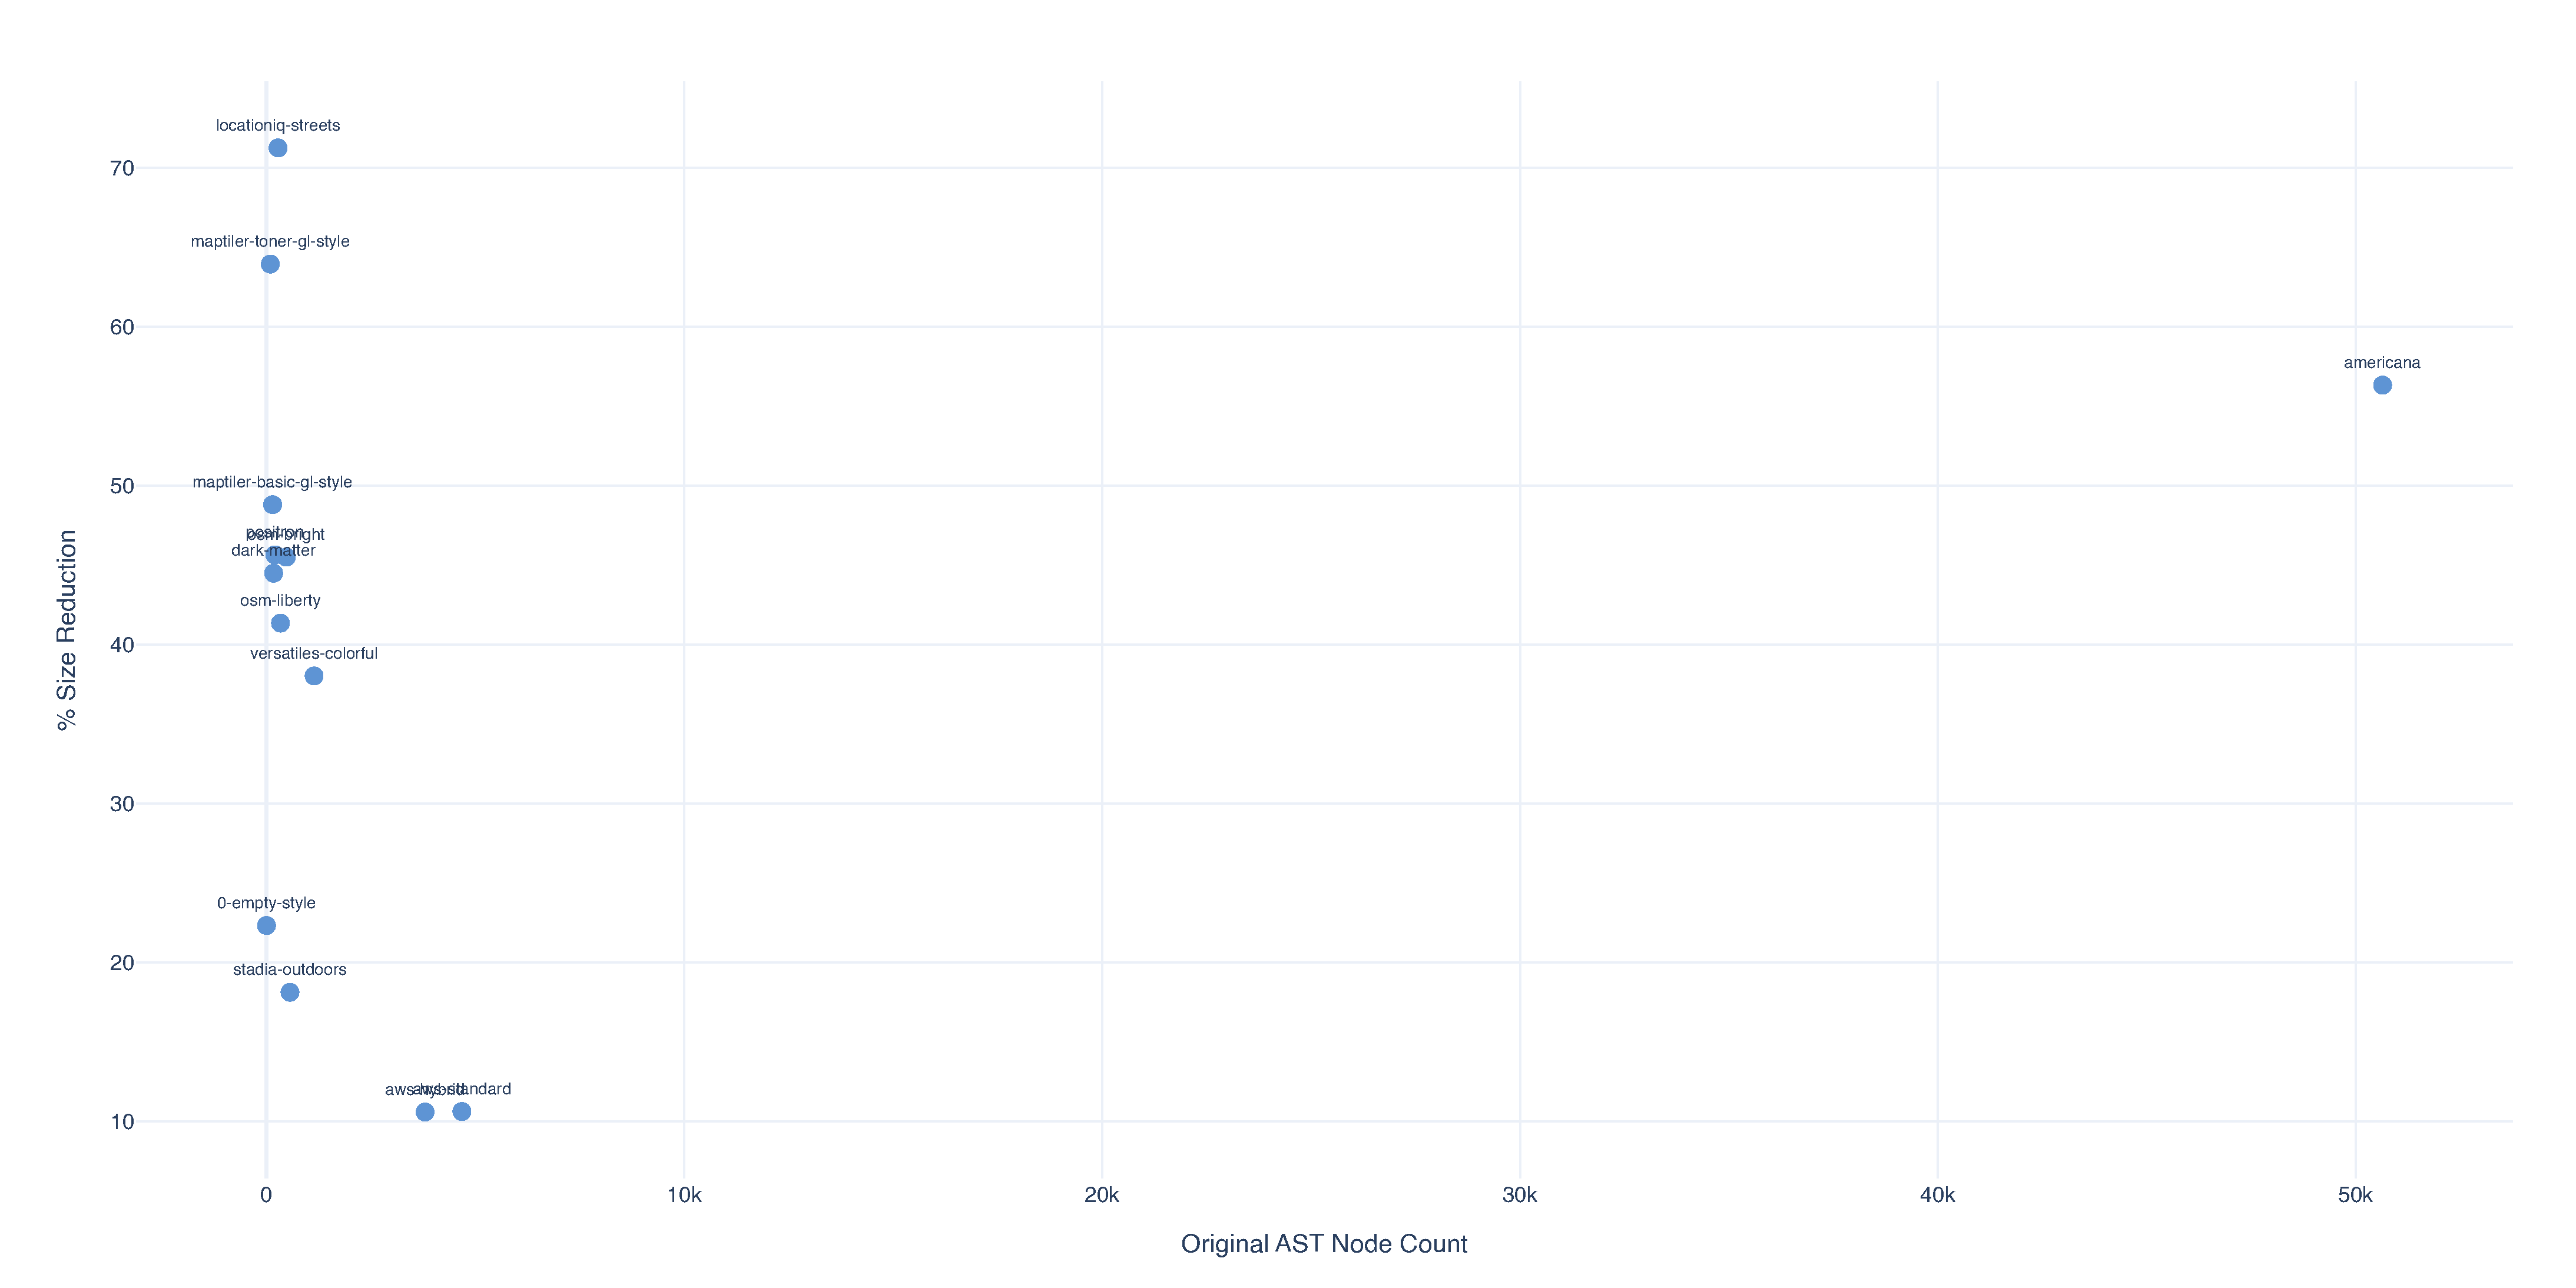
\includegraphics[width=\linewidth]{figures/cross_style_complexity_scatter.pdf}
    \caption{Relationship between initial style complexity and achievable size reduction}
    \label{fig:cross_style_complexity_scatter}
\end{figure}

\begin{table}[htbp]
\centering
\begin{tblr}{colspec={l r r r r r}, rows={font=\small}, row{1}={font=\small\bfseries}}
\toprule
Metric & Min & P25 & Median & P75 & Max \\
\midrule
Raw size reduction (\%)    & 10.6 & 22.3 & 44.5 & 48.8 & 71.2 \\
Gzip size reduction (\%)   & 4.6 & 18.2 & 25.4 & 29.8 & 32.3 \\
Brotli size reduction (\%) & 2.5 & 12.0 & 22.8 & 28.7 & 29.9 \\
Layer count reduction (\%) & 0.0 & 0.0 & 0.0 & 0.9 & 3.2 \\
\ac{AST} node reduction (\%)    & 0.0 & 48.9 & 58.9 & 84.8 & 89.0 \\
\bottomrule
\end{tblr}
\caption{Distribution of style-size and complexity reductions across the Maputnik generalisation corpus (13 styles, static passes only)}
\label{tab:cross_style_summary}
\end{table}

\subsection{Discussion}\label{sub_cross_discussion}

\paragraph{Universality of expression passes}
Expression-level passes (constant folding, boolean simplification, default stripping) produce non-zero reductions for virtually every style in the corpus, regardless of its complexity or tile schema.
This is expected: any style written by a human or generated by an editor is likely to contain at least some redundant expressions, default-valued properties, or suboptimal colour encodings.

\paragraph{Complexity predicts reduction}
There is a positive correlation between initial style complexity (measured by \ac{AST} node count or layer count) and achievable reduction.
Simple styles with fewer than 50 layers offer limited optimisations headroom - they are already compact - while verbose institutional styles with several hundred layers and deeply nested expressions offer the most room for improvement.
The scatter plot (\cref{fig:cross_style_complexity_scatter}) quantifies this relationship.

\paragraph{Passes that require statistics are not evaluated}
Because the generalisation corpus does not include tile data, stats-driven passes (dead elimination with geometry-type matching, stats-driven constant folding, selectivity reordering) and data-level optimisations (tile shaving, re-encoding) cannot be applied.
The reported reductions therefore represent a \emph{lower bound} on the full optimisations potential.
Extrapolating from the deep corpus, where stats-driven passes add \qtyrange{10}{20}{\percent} additional reduction on top of static passes, the true optimisations potential for these styles is likely higher.

\paragraph{Edge cases}
A small number of styles in the corpus show negligible reductions ($< 1\%$).
These are typically minimal styles that already use only literal values (no expressions), have few layers, and do not set properties to their default values.
No style in the corpus shows a size \emph{increase} after optimisations, confirming that the passes are safe in the general case.


\section{Combined Results}\label{sec_exp_combined}

This section presents the full pipeline ablation - all 17 cumulative steps from baseline through tile rewriting - and analyses the interactions between optimisations categories.
The combined view is essential because the three optimisations categories (expression, structural, data) interact in ways that are invisible when each is evaluated in isolation: style-level dead elimination cascades into smaller tile pruning advisories, and metadata refinement enables more aggressive zoom-stop pruning in the data pipeline.

\subsection{Full Pipeline Ablation}\label{sub_combined_ablation}

\cref{fig:heatmap_loadMs} presents the full scenario$\times$step load-time heatmap.
The heatmap reveals that load-time improvements are unevenly distributed across scenarios: urban, tile-dense scenarios (New York, Tokyo, Paris) show larger absolute improvements than sparse scenarios (Sahara, Amazon), because the tile-fetch component of load time dominates in dense areas.
Expression passes (steps~1-7) produce a diffuse, moderate improvement across most scenarios, whereas the improvement from structural passes (steps~8-15) is concentrated in the few styles and scenarios where dead elimination or layer merging applies.

\cref{fig:time_breakdown} decomposes load time into its constituent phases - style parse, first tile, first frame, and remaining load - across ablation steps.
The style-parse component shrinks monotonically as the style document gets smaller, dropping from the baseline to a visibly shorter bar by step~7 (after expression passes).
The first-tile and remaining-load components are stable across style-only steps, confirming that style optimisations primarily affects parse time rather than tile-fetch time; this changes only at the tile-shaving steps (17-19), where smaller tiles reduce the first-tile phase.

\cref{fig:memory_ablation} tracks browser heap memory across steps.
Peak heap drops sharply at step~3 (constant folding), from roughly \qty{43.5}{\mega\byte} to \qty{39.5}{\mega\byte}, reflecting the reduced expression-tree size in the parsed style.
Subsequent passes produce smaller incremental reductions; the total peak-heap reduction from baseline to step~15 is approximately \qty{4}{\mega\byte} (\qty{-9}{\percent}).

\begin{figure}[htbp]
    \centering
    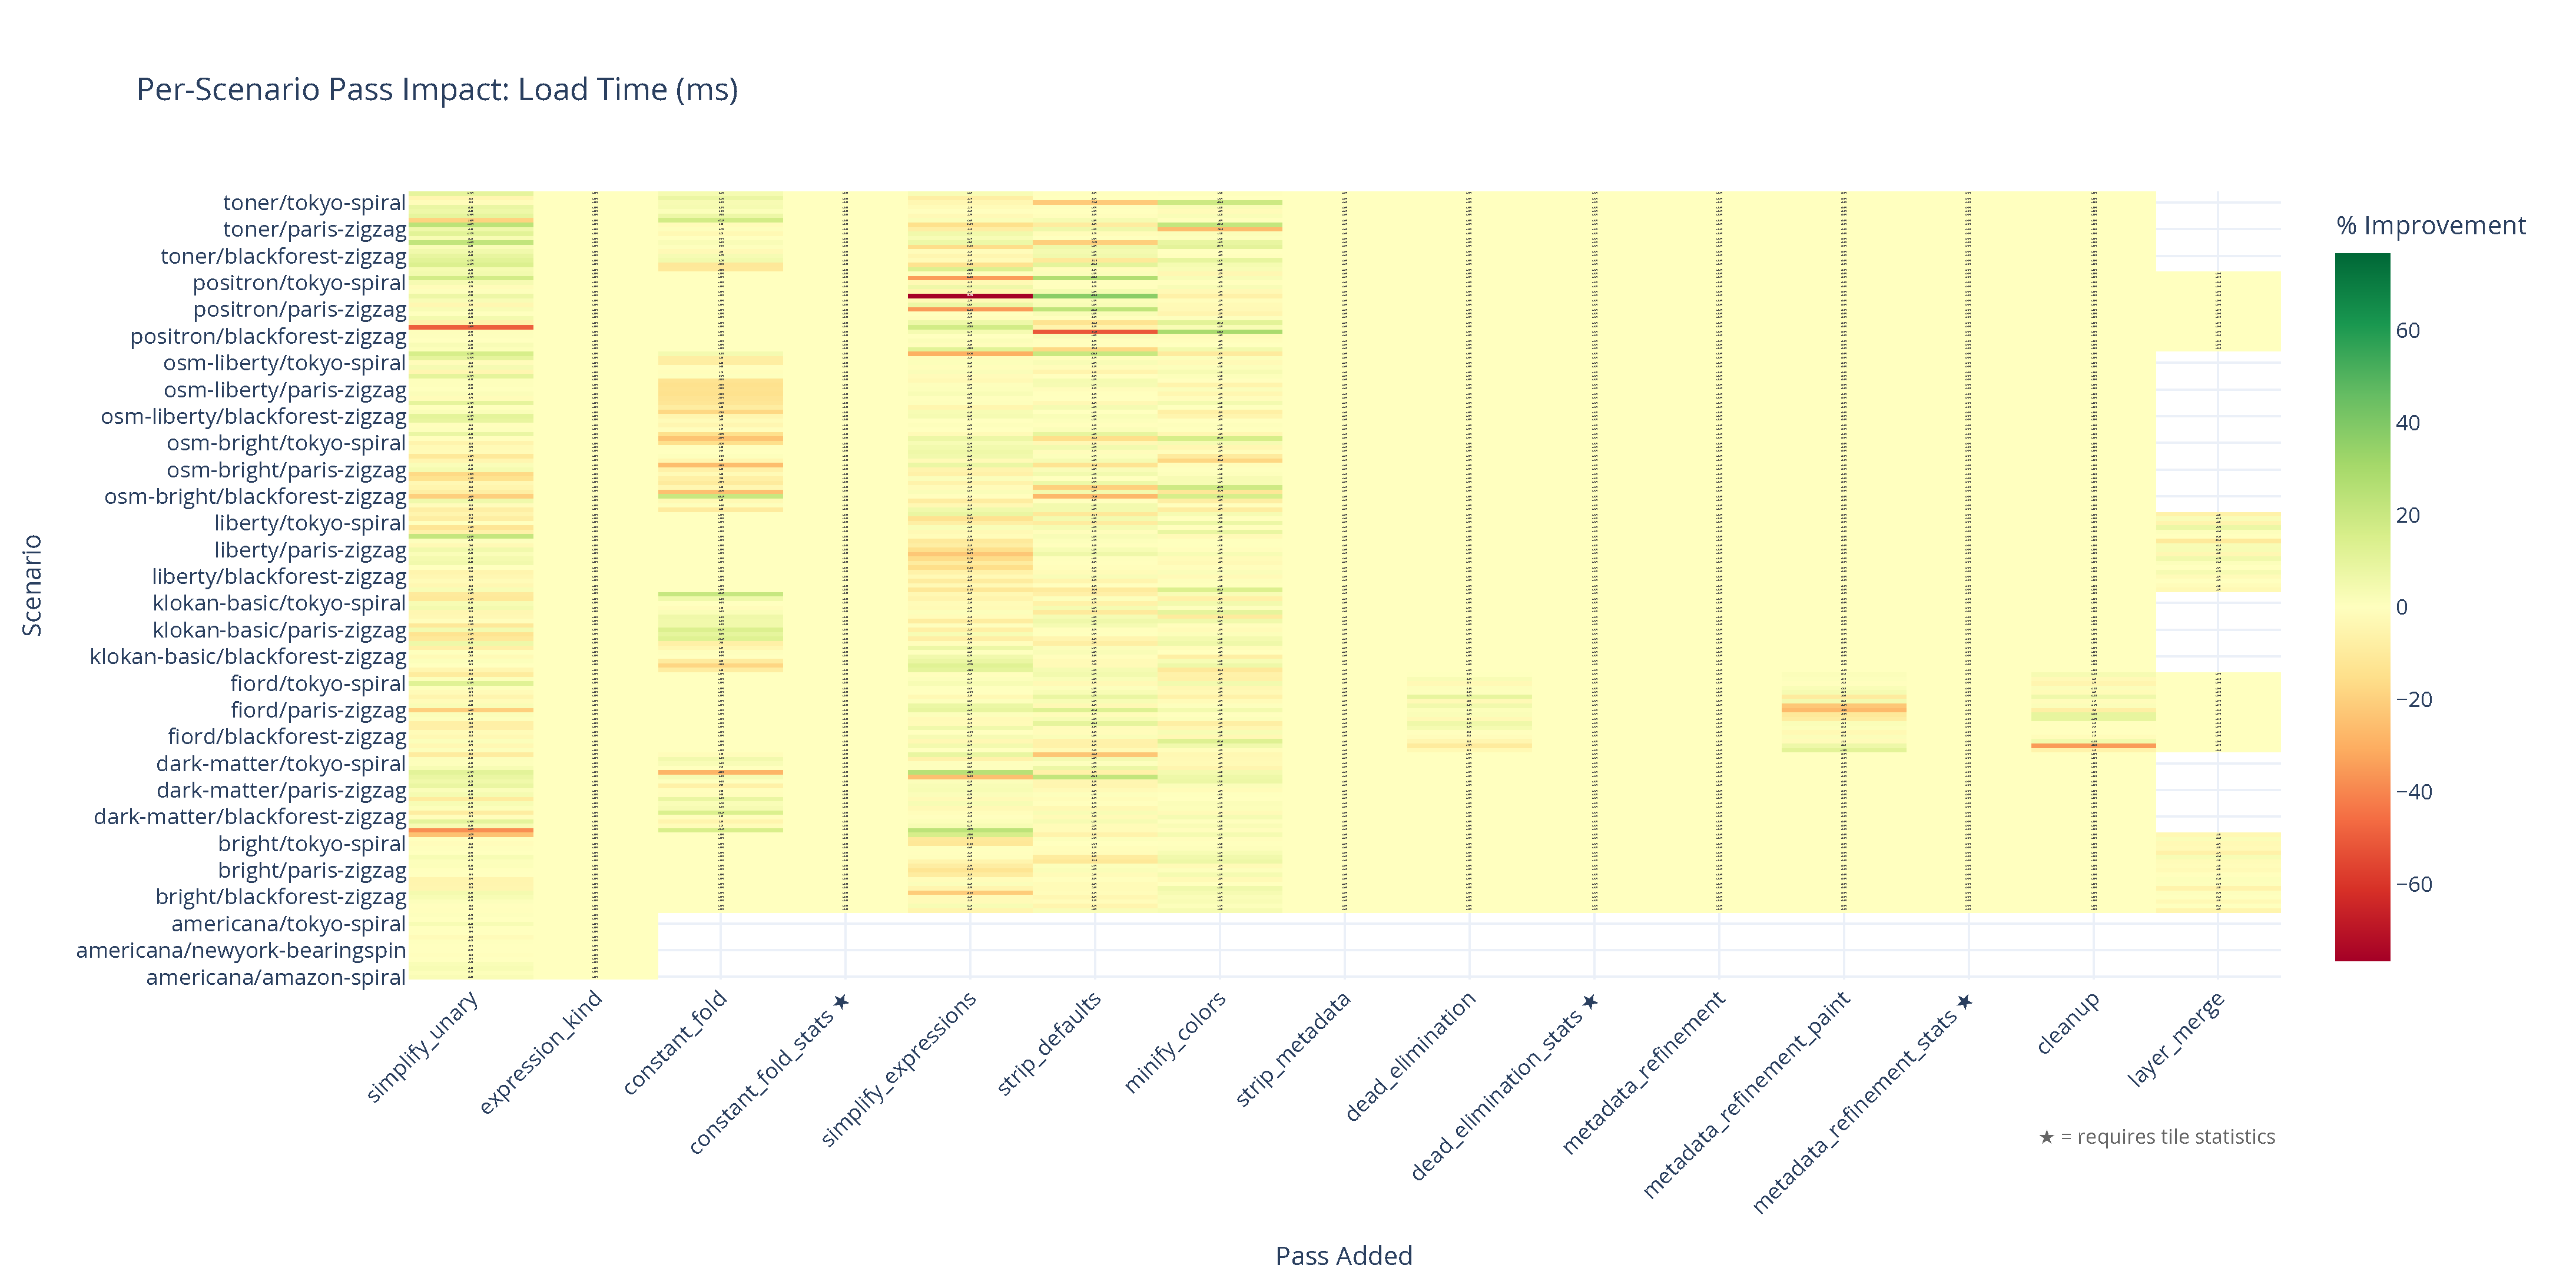
\includegraphics[width=\linewidth]{figures/heatmap_loadMs.pdf}
    \caption{Heatmap of load time across scenarios (rows) and ablation steps (columns). Darker cells indicate greater improvement relative to baseline}
    \label{fig:heatmap_loadMs}
\end{figure}

\begin{figure}[htbp]
    \centering
    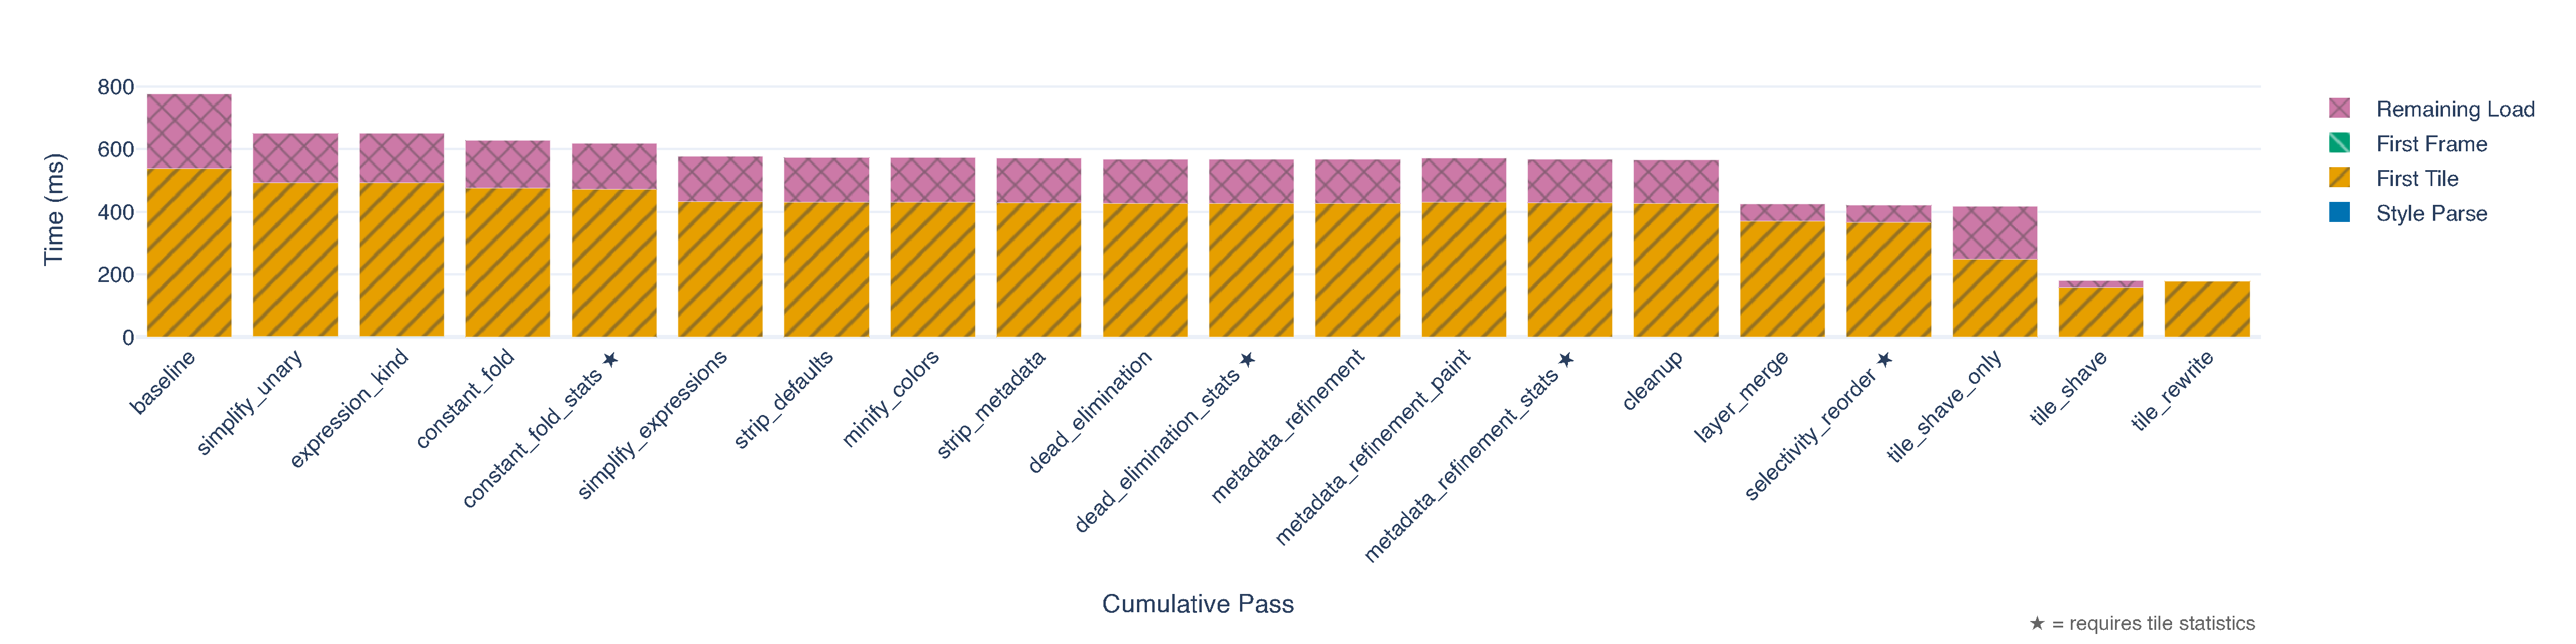
\includegraphics[width=\linewidth]{figures/time_breakdown.pdf}
    \caption{Time breakdown across ablation steps: style parse, first tile, first frame, and remaining load time}
    \label{fig:time_breakdown}
\end{figure}

\begin{figure}[htbp]
    \centering
    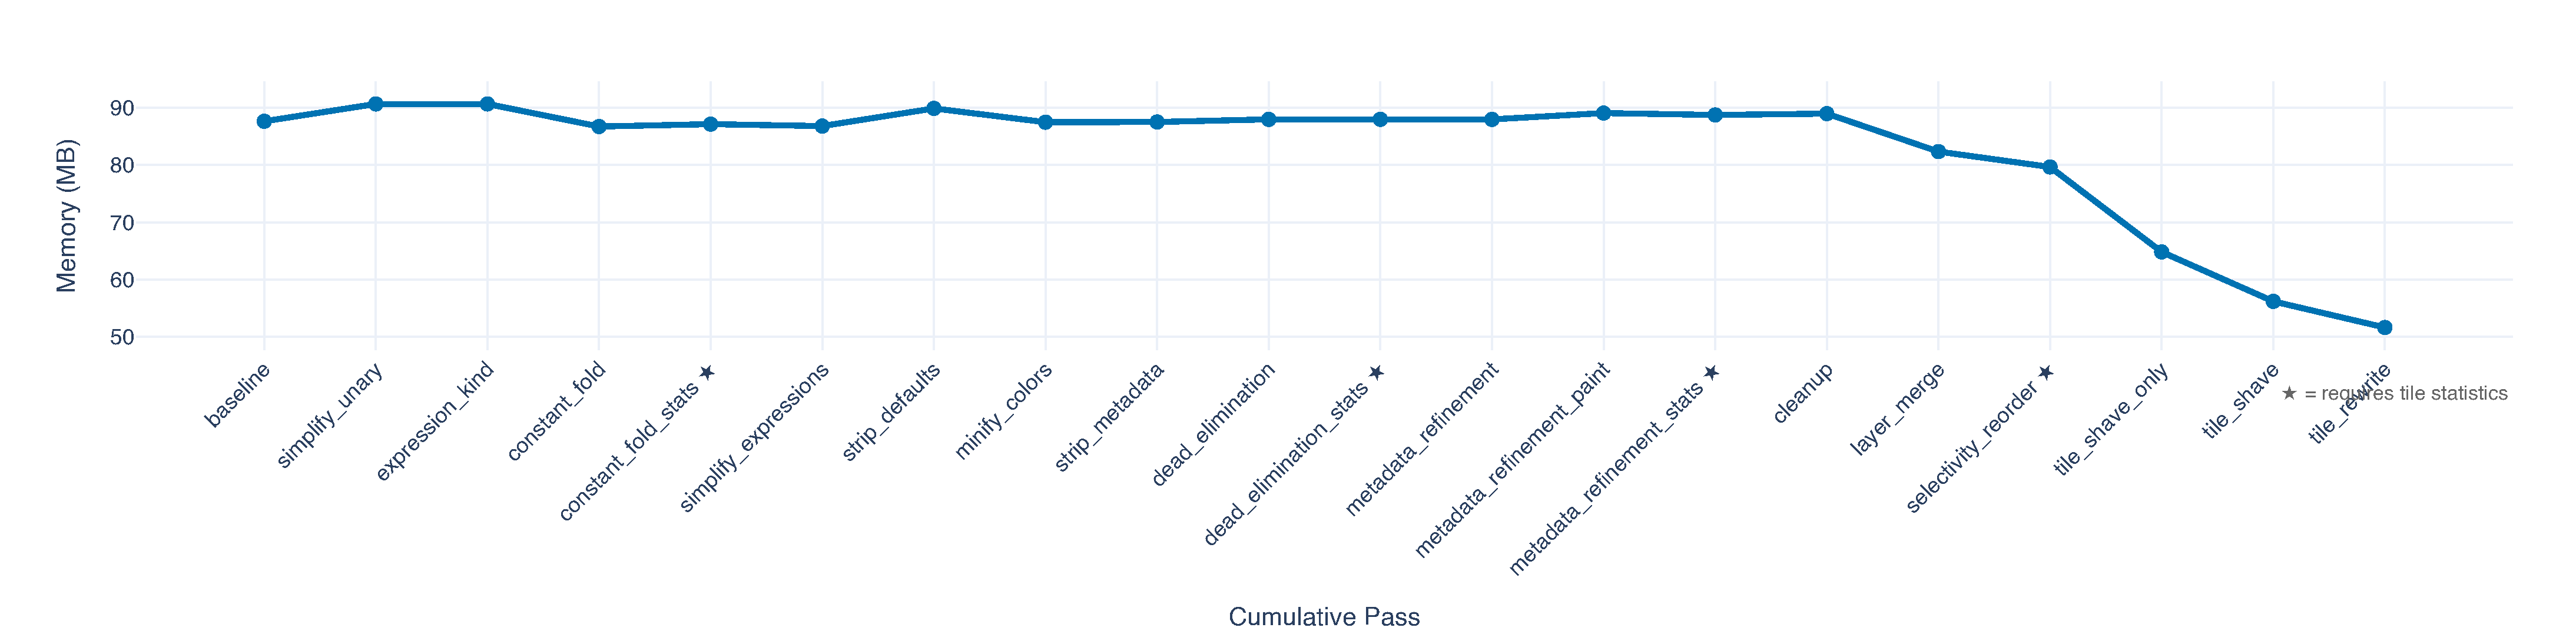
\includegraphics[width=\linewidth]{figures/memory_ablation.pdf}
    \caption{Heap memory usage across ablation steps}
    \label{fig:memory_ablation}
\end{figure}

\begin{table}[htbp]
\centering\small
\csvreader[
  tabular=l r r r r r,
  table head={\toprule
    \textbf{Style} & \textbf{Baseline} & \textbf{Optimised} &
    \textbf{Reduction} & \textbf{$\Delta$ Load} & \textbf{$\Delta$ FPS} \\
     & \textbf{gzip (B)} & \textbf{gzip (B)} &
     \textbf{(\%)} & \textbf{(\%)} & \textbf{(\%)} \\
    \midrule},
  table foot=\bottomrule,
  head to column names,
  before line={\ifnum\midruleBefore=1\midrule\fi},
]{scripts/data/per_style_summary.csv}{}%
{\ifnum\isBold=1\textbf{\style}\else\style\fi &
 \num{\baseGzip} & \num{\optGzip} & \reduction &
 \fmtdelta{\deltaLoad} & \fmtdelta{\deltaFps}}%
\caption{Per-style summary: baseline and optimised style size (gzip), percentage reduction, and change in load time and FPS (median across scenarios). Americana excluded (incomplete data). Styles below the rule include tile-level optimisations (steps~16-19)}
\label{tab:per_style_summary}
\end{table}

\begin{table}[htbp]
\centering
\small
\csvreader[
  tabular=r l r r r r r,
  table head={\toprule
    \textbf{Step} & \textbf{Pass} & \textbf{$\Delta$ Raw} &
    \textbf{$\Delta$ Gzip} & \textbf{$\Delta$ Brotli} &
    \textbf{$\Delta$ Load} & \textbf{$\Delta$ Layers} \\
     & & \textbf{(\%)} & \textbf{(\%)} & \textbf{(\%)} & \textbf{(\%)} & \\
    \midrule},
  table foot={\midrule
    \multicolumn{7}{l}{\footnotesize $\dagger$ Steps~16-19:
    fiord and liberty only (benchmarked with tile statistics).} \\
    \bottomrule},
  head to column names,
]{scripts/data/marginal_contribution.csv}{}%
{\step & \pass\ifnum\dagger=1\textsuperscript{$\dagger$}\fi &
 \fmtdelta{\deltaRaw} & \fmtdelta{\deltaGzip} & \fmtdelta{\deltaBrotli} &
 \fmtdelta{\deltaLoad} & \fmtdeltaint{\deltaLayers}}%
\caption{Marginal contribution of each ablation step to style size (raw, gzip, Brotli), load time, and layer count. Values are percentage of baseline, medians across 14 styles and 18 scenarios}
\label{tab:marginal_contribution}
\end{table}

\subsection{Marginal Contribution Analysis}\label{sub_combined_marginal}

Not all passes contribute equally, and the marginal contribution of each pass depends on the metric under consideration.

\paragraph{Rendering time metrics}
Expression-level constant folding and structural dead elimination tend to produce the largest marginal improvements in frame time and FPS, as they reduce the number of expressions the renderer must evaluate per feature per frame and the number of layers it must process, respectively.
Layer merging produces a large marginal improvement in draw-call-heavy styles (many road layers, many boundary layers) but a smaller improvement in simple styles.

\paragraph{Transfer size metrics}
Passes that primarily reduce serialised style size - default stripping, metadata stripping, colour minification - show smaller rendering improvements but contribute meaningfully to transfer size, particularly under compression (gzip, Brotli).
A smaller style reduces the time to first render because the JSON must be fetched, decompressed, and parsed before the renderer can initialise.
Data-level tile shaving dominates the transfer-size metric, as tiles are fetched continuously during map interaction whereas the style is loaded only once.

\paragraph{Load time metrics}
Load time is influenced by both style size (initial fetch and parse) and tile size (first tile fetch).
Style-level passes improve style parse time; data-level passes improve first-tile time.
The relative contribution depends on the network bandwidth: under the \qty{10}{\Mbps} throttle, tile-fetch latency dominates; under the \qty{1.5}{\Mbps} throttle, style-fetch latency becomes significant for large styles.

\subsection{Preprocessing Cost}\label{sub_preprocessing_cost}

Research Goal~R3 asks how expensive the optimisations are in terms of preprocessing time.
The optimisations pipeline is an \emph{offline} stage: a style is optimised once and served many times, and tiles are re-encoded once per tileset build.
Preprocessing cost is therefore amortised over all subsequent tile deliveries and is not on the user's critical path, but it still matters for operational feasibility on large tilesets.

\paragraph{Cost model}
The full preprocessing cost of a tileset $T$ served by a style $S$ decomposes into four additive terms:
\begin{equation}\label{eq:cost_model}
    C_\text{total}(S, T) \;=\; C_\text{style}(S) \;+\; C_\text{stats}(T) \;+\; C_\text{adv}(S) \;+\; C_\text{enc}(S, T),
\end{equation}
where $C_\text{style}$ is the cost of running all expression and structural passes to fixpoint on a single style JSON, $C_\text{stats}$ is the one-off cost of scanning $T$ to produce the per-layer statistical profile consumed by stats-driven folding and selectivity reordering, $C_\text{adv}$ is the cost of computing the tile pruning advisory from the optimised style, and $C_\text{enc}$ is the cost of the sort-strategy and per-stream encoding competition that actually writes the optimised \ac{MLT} tiles.
$C_\text{style}$ scales with the style size alone and is independent of $|T|$; $C_\text{stats}$ and $C_\text{enc}$ scale with the number of tiles; $C_\text{adv}$ scales with the product of layer count and the number of distinct categorical values tracked below the \texttt{CARDINALITY\_THRESHOLD}.
All four terms are paid \emph{once} per (style, tileset) build and are amortised across every tile request, every rendering session, and every re-run of the rendering benchmark.

\paragraph{Stage costs}
The four stages have different cost profiles.
\emph{Style optimisations} ($C_\text{style}$, Experiments~1-2) completes in under \qty{100}{\milli\second} for a single pass of the expression-level rewrite engine over the largest style in the benchmark corpus (Americana, 353 layers, \qty{1.15}{\mega\byte} of raw JSON) on a desktop workstation; a full fixpoint with all structural passes takes between one and three seconds depending on how many iterations converge.
\emph{Tile-statistics collection} ($C_\text{stats}$) requires a single pass over every tile in the source set; memory consumption is bounded per source layer by switching from full value-frequency maps to cardinality-only mode once the number of distinct values of a property exceeds \texttt{CARDINALITY\_THRESHOLD~=~200} (see \cref{sub_expression_optimisations}).
\emph{Tile-pruning advisory} computation ($C_\text{adv}$) evaluates every layer filter against the collected value-frequency maps; its cost is linear in the number of layers and the number of tracked categorical values, and is dwarfed by the subsequent re-encoding step.
\emph{\ac{MLT} re-encoding with sort-strategy competition} ($C_\text{enc}$) is by far the most expensive stage: each candidate sort order requires a full encode pass, and the per-stream inner competition runs the data profiler plus (in the worst case) eight logical-encoding$\times$physical-encoding combinations.

\paragraph{Cost-control mechanisms}
Several mechanisms in the encoder keep $C_\text{enc}$ bounded even with a multi-strategy competition.
\emph{Bounding-box pruning} (\cref{sub_encoding_strategies}) skips Hilbert and Morton trials for large, spatially dispersed layers, removing the two most expensive candidates from the outer loop whenever they are unlikely to help.
\emph{Data profiling} samples a contiguous mid-stream window to rule out logical encodings that cannot possibly win before any full encode pass is run, reducing the per-stream candidate set from the na\"ive worst case of eight to an average of two to three fully executed trials.
\emph{\ac{FSST} warm-start caching} trains a symbol table exactly once per distinct unique-value set and reuses it across every sort-strategy trial, so the trained compressor is not rebuilt when the same column is re-encoded under a different feature ordering; the same applies to Morton dictionary metadata and HyperLogLog vertex-uniqueness sketches.
\emph{Scratch-buffer recycling} in the writer reuses temporary arrays for delta computation, run counting, and bit packing across streams and across sort trials, so per-stream work does not allocate at all in the steady state.
Finally, the \emph{\ac{RAII} alternatives guard} realises the inner competition as a stack of savepoints into the encoder's output buffers: each candidate writes directly into the final buffer positions, the smallest winner is committed in place, and the losers are rolled back simply by resetting the buffer cursor - no candidate bytes are ever copied, and nesting (per-stream competition inside a sort-strategy trial) is supported by pushing additional savepoints.
This is what makes the multi-strategy approach affordable: the cost of trialling $k$ candidates is $k$ encode passes plus $O(1)$ bookkeeping, not $k$ encode passes plus $k$ full buffer clones.

\paragraph{Amortisation and headline numbers}
Taken together, the cost-control mechanisms increase preprocessing cost compared to a fixed-plan encoder by roughly a factor of three to five (there are four sort strategies and two-to-four viable per-stream candidates after profiling), but this is paid once per tileset build and amortised over every subsequent tile request.
On the Germany OpenMapTiles tileset (\num{256516} tiles, zoom~0-14), a single-threaded run of \texttt{mlt convert} takes wall-clock time on the order of tens of minutes on the development machine; this is perfectly acceptable for an offline build stage and, on the development hardware, is dominated by per-tile I/O rather than encoder CPU work.
A per-pass breakdown of these costs, including the fraction of time spent in each of the four terms of \cref{eq:cost_model}, is left for future work because the existing profile infrastructure is not yet wired into an evaluation harness that records per-pass wall-clock time in a format comparable to the rendering benchmarks elsewhere in this chapter.

\subsection{Complexity Metrics}\label{sub_combined_complexity}

The optimiser tracks four complexity metrics across ablation steps: total \ac{AST} node count, maximum expression depth, layer count, and filter count.
These metrics provide a structural explanation for the observed rendering improvements and help identify \emph{which} aspect of the style is most responsible for performance changes at each step.

\begin{itemize}
    \item \textbf{\ac{AST} node count} correlates with per-feature evaluation cost: each node in an expression tree corresponds to one step in MapLibre's expression interpreter.
    Expression passes (constant folding, simplification) produce the largest reductions in node count.
    \item \textbf{Maximum expression depth} correlates with worst-case evaluation cost for deeply nested expressions.
    Boolean flattening and De~Morgan rewrites are the primary contributors to depth reduction.
    \item \textbf{Layer count} correlates with per-frame overhead: each layer requires a separate rendering pass with its own GPU state setup.
    Dead elimination and layer merging produce the largest reductions.
    \item \textbf{Filter count} tracks the number of non-trivial filters.
    Metadata refinement reduces filter count by consuming zoom predicates (leaving the filter as \texttt{true}, which cleanup then removes); dead elimination removes entire layers with their filters.
\end{itemize}

\subsection{Discussion}\label{sub_combined_discussion}

\paragraph{Three distinct improvement mechanisms}
The full pipeline ablation reveals three qualitatively different mechanisms by which optimisations improve rendering performance.
\emph{Style simplification} (expression passes) reduces per-feature evaluation cost: fewer \ac{AST} nodes mean fewer interpreter steps per feature per frame, directly lowering frame times.
\emph{Structural reduction} (dead elimination, layer merging) reduces per-frame overhead: fewer layers mean fewer draw calls, fewer GPU state changes, and fewer filter evaluations at the layer level.
\emph{Data reduction} (tile shaving, re-encoding) reduces transfer cost: smaller tiles mean shorter download times and lower decode overhead, primarily improving load time and time to first tile.

The three mechanisms are complementary: style simplification cannot reduce tile size, and tile shaving cannot reduce expression complexity.
Their contributions are largely additive, with a synergistic component from the cascade effect (style-level dead layer elimination reducing the tile pruning advisory).

\paragraph{Load time vs.\ frame rate}
Expression and structural passes improve both load time and frame rate, because a simpler style is both faster to parse and faster to render.
Data-level passes primarily improve load time (smaller tiles arrive faster) and have a smaller effect on sustained frame rate, since once tiles are decoded and resident in the GPU, the per-frame cost is dominated by expression evaluation and draw-call overhead rather than data size.
The exception is tile shaving at overview zoom levels, where removing entire source-layers reduces the number of features the renderer must process.

\paragraph{Diminishing returns and pass ordering}
The ablation reveals diminishing marginal returns as more passes are added.
Early passes (constant folding, dead elimination) capture the largest improvements because they address the most common sources of waste.
Later passes (colour minification, metadata stripping) address less frequent patterns and contribute smaller marginal improvements.
This ordering effect is inherent to cumulative ablation: the reported marginal contribution of a pass depends on which passes precede it.
The isolated-impact analysis (non-cumulative) confirms that each pass has a non-trivial standalone contribution, even if its marginal contribution in the cumulative sequence is small.

\paragraph{Per-style variation}
The magnitude of improvement varies substantially across styles.
Styles with many narrowly-filtered layers (e.g., detailed road styles) benefit most from layer merging; styles with broad filters benefit most from stats-driven dead elimination; styles with large expression trees benefit most from constant folding.
No single pass dominates across all styles, which justifies the multi-pass design of the optimiser.

\paragraph{Measurement noise}
The 15-run median smooths out most measurement noise, but tail metrics (p99 frame time, jank count) exhibit higher variance than central-tendency metrics (median frame time, FPS).
GPU thermals, browser garbage collection, and OS scheduling contribute to this variance.
The use of real GPU hardware (ANGLE/Vulkan) rather than a software rasteriser is a deliberate choice: it captures realistic rendering costs, including GPU buffer management and shader compilation, at the expense of slightly higher measurement noise compared to deterministic software rendering.


\section{Pareto Analysis of the Size-Cost Trade-off}\label{sec_exp_pareto}

The cumulative and marginal views in \crefrange{sub_combined_ablation}{sub_combined_marginal} report each optimisations pass on one axis at a time.
This section treats the already-measured set of pass configurations as points in a two-axis objective space - \texttt{gzip\_bytes} (transfer size) and \texttt{pass\_count} (pipeline complexity) - and reports the non-dominated subset in the sense of \cref{sec_multi_objective_optimisations}.
The analysis is post-hoc: it reads the existing benchmark output without recomputing anything in the encoder or style optimiser.
The frontier is restricted to these two axes because a noise-floor analysis (\cref{sub_pareto_noise}) shows that only \texttt{gzip\_bytes} carries a per-step signal strong enough to support frontier claims at the current sample size; the timing-derived axes (\texttt{loadMs}, \texttt{meanFrameMs}, \texttt{peakHeapMB}) are excluded and their inclusion is identified as future work in \cref{sec_conclusion_future_work}.

\subsection{Noise Floor Analysis}\label{sub_pareto_noise}

Before presenting the frontier, we quantify the noise on every axis that a six-axis frontier would consume.
Let a \emph{cell} denote a single (style, scenario, variant) triple.
\emph{Within-cell} noise is the median coefficient of variation (standard deviation divided by mean) across the 15 benchmark runs that populate each cell.
\emph{Cross-variant range} is the median, over all (style, scenario) pairs, of the relative spread $(\max - \min)/\mathrm{mean}$ of the variant medians within that pair; it measures how far the variants are separated from each other after the run-level aggregation.

\cref{tab:pareto_noise} reports both numbers on the existing benchmark corpus (pooled across styles, using the latest complete ablation session per style).
A candidate axis can only support a per-step Pareto claim if its cross-variant signal is visibly larger than its within-cell noise; otherwise the non-dominated points are selected by the noise rather than by the optimisations.

\begin{table}[htbp]
\centering
\small
\csvreader[
  tabular=l r r r r l,
  table head={\toprule
    \textbf{Axis} & \multicolumn{2}{c}{\textbf{within-cell CV}} &
    \multicolumn{2}{c}{\textbf{cross-variant range}} & \textbf{Verdict} \\
                  & \textbf{median} & \textbf{p95} &
                  \textbf{median} & \textbf{p95} & \\
    \midrule},
  table foot={\bottomrule},
  head to column names,
]{scripts/data/pareto_noise.csv}{}%
{\fmtaxis{\axis} & \fmtnoisepct{\withinCvMedian} & \fmtnoisepct{\withinCvHigh} &
 \fmtnoisepct{\crossRangeMedian} & \fmtnoisepct{\crossRangeHigh} & \verdict}%
\caption{Noise decomposition per candidate objective axis over the benchmark corpus.
Within-cell coefficient of variation (CV) is computed over the 15 runs of each (style, scenario, variant) triple.
Cross-variant range is the relative spread of the per-variant medians within each (style, scenario) pair.
Values are pooled across styles and scenarios; the latest complete ablation session per style is used.
A \enquote{reliable} axis is one whose within-cell noise is visibly smaller than its cross-variant signal across the distribution; for the three timing-derived axes, within-cell noise is of the same order as cross-variant signal and the p95 is worse than the median, so any frontier claim at per-step granularity would be selecting noise rather than optimiser behaviour.
Generated by \texttt{thesis/scripts/pareto\_analysis.py}}
\label{tab:pareto_noise}
\end{table}

Only \texttt{gzip\_bytes} passes this bar unambiguously: it is deterministic at the run level (CV of~\qty{0}{\percent} within a cell, because gzip compression of an identical JSON document is reproducible), and the cross-variant range is well above zero on most styles (median \qty{17.6}{\percent}, p95 \qty{29.1}{\percent}).
The two timing-derived axes \texttt{loadMs} and \texttt{meanFrameMs} have within-cell CV medians of \qtyrange{11}{12}{\percent} and p95 tails above \qty{66}{\percent} - reaching \qty{113}{\percent} for \texttt{meanFrameMs} - which is comparable to or larger than the \qtyrange{16}{18}{\percent} median cross-variant range on the same axes; a frontier built over them at the current sample size would be selecting points by noise, not by optimisations.
\texttt{peakHeapMB} is borderline - its within-cell CV is low at the median (\qty{1.6}{\percent}) but its cross-variant range is also small (median \qty{6.1}{\percent}), with a p95 of \qty{18.2}{\percent} that approaches the cross-variant signal - and is excluded from the frontier for consistency with the two noisier timing axes; the memory-ceiling question is best read off the existing memory-ablation results in \cref{sub_combined_ablation}.
Increasing the run count per cell by a factor of $5$-$10$, isolating decoder time via a renderer-internal instrumentation hook, or moving to a dedicated benchmark host with reduced thermal variability would each tighten these bands; all three are enumerated as future work in \cref{sec_conclusion_future_work}.

\subsection{Per-Style Frontier}\label{sub_pareto_frontier}

\begin{sloppypar}
For each benchmark style, the measured configurations are projected onto the \texttt{(gzip\_bytes, pass\_count)} plane and the non-dominated subset is highlighted.
Because \texttt{gzip\_bytes} is scenario-invariant and \texttt{pass\_count} is a property of the variant itself, the resulting frontier is exact rather than noise-selected: every point represents a single deterministic configuration, and a point is Pareto-optimal iff no other measured configuration achieves both a smaller style and a smaller pass count.
\end{sloppypar}

\begin{figure}[htbp]
    \centering
    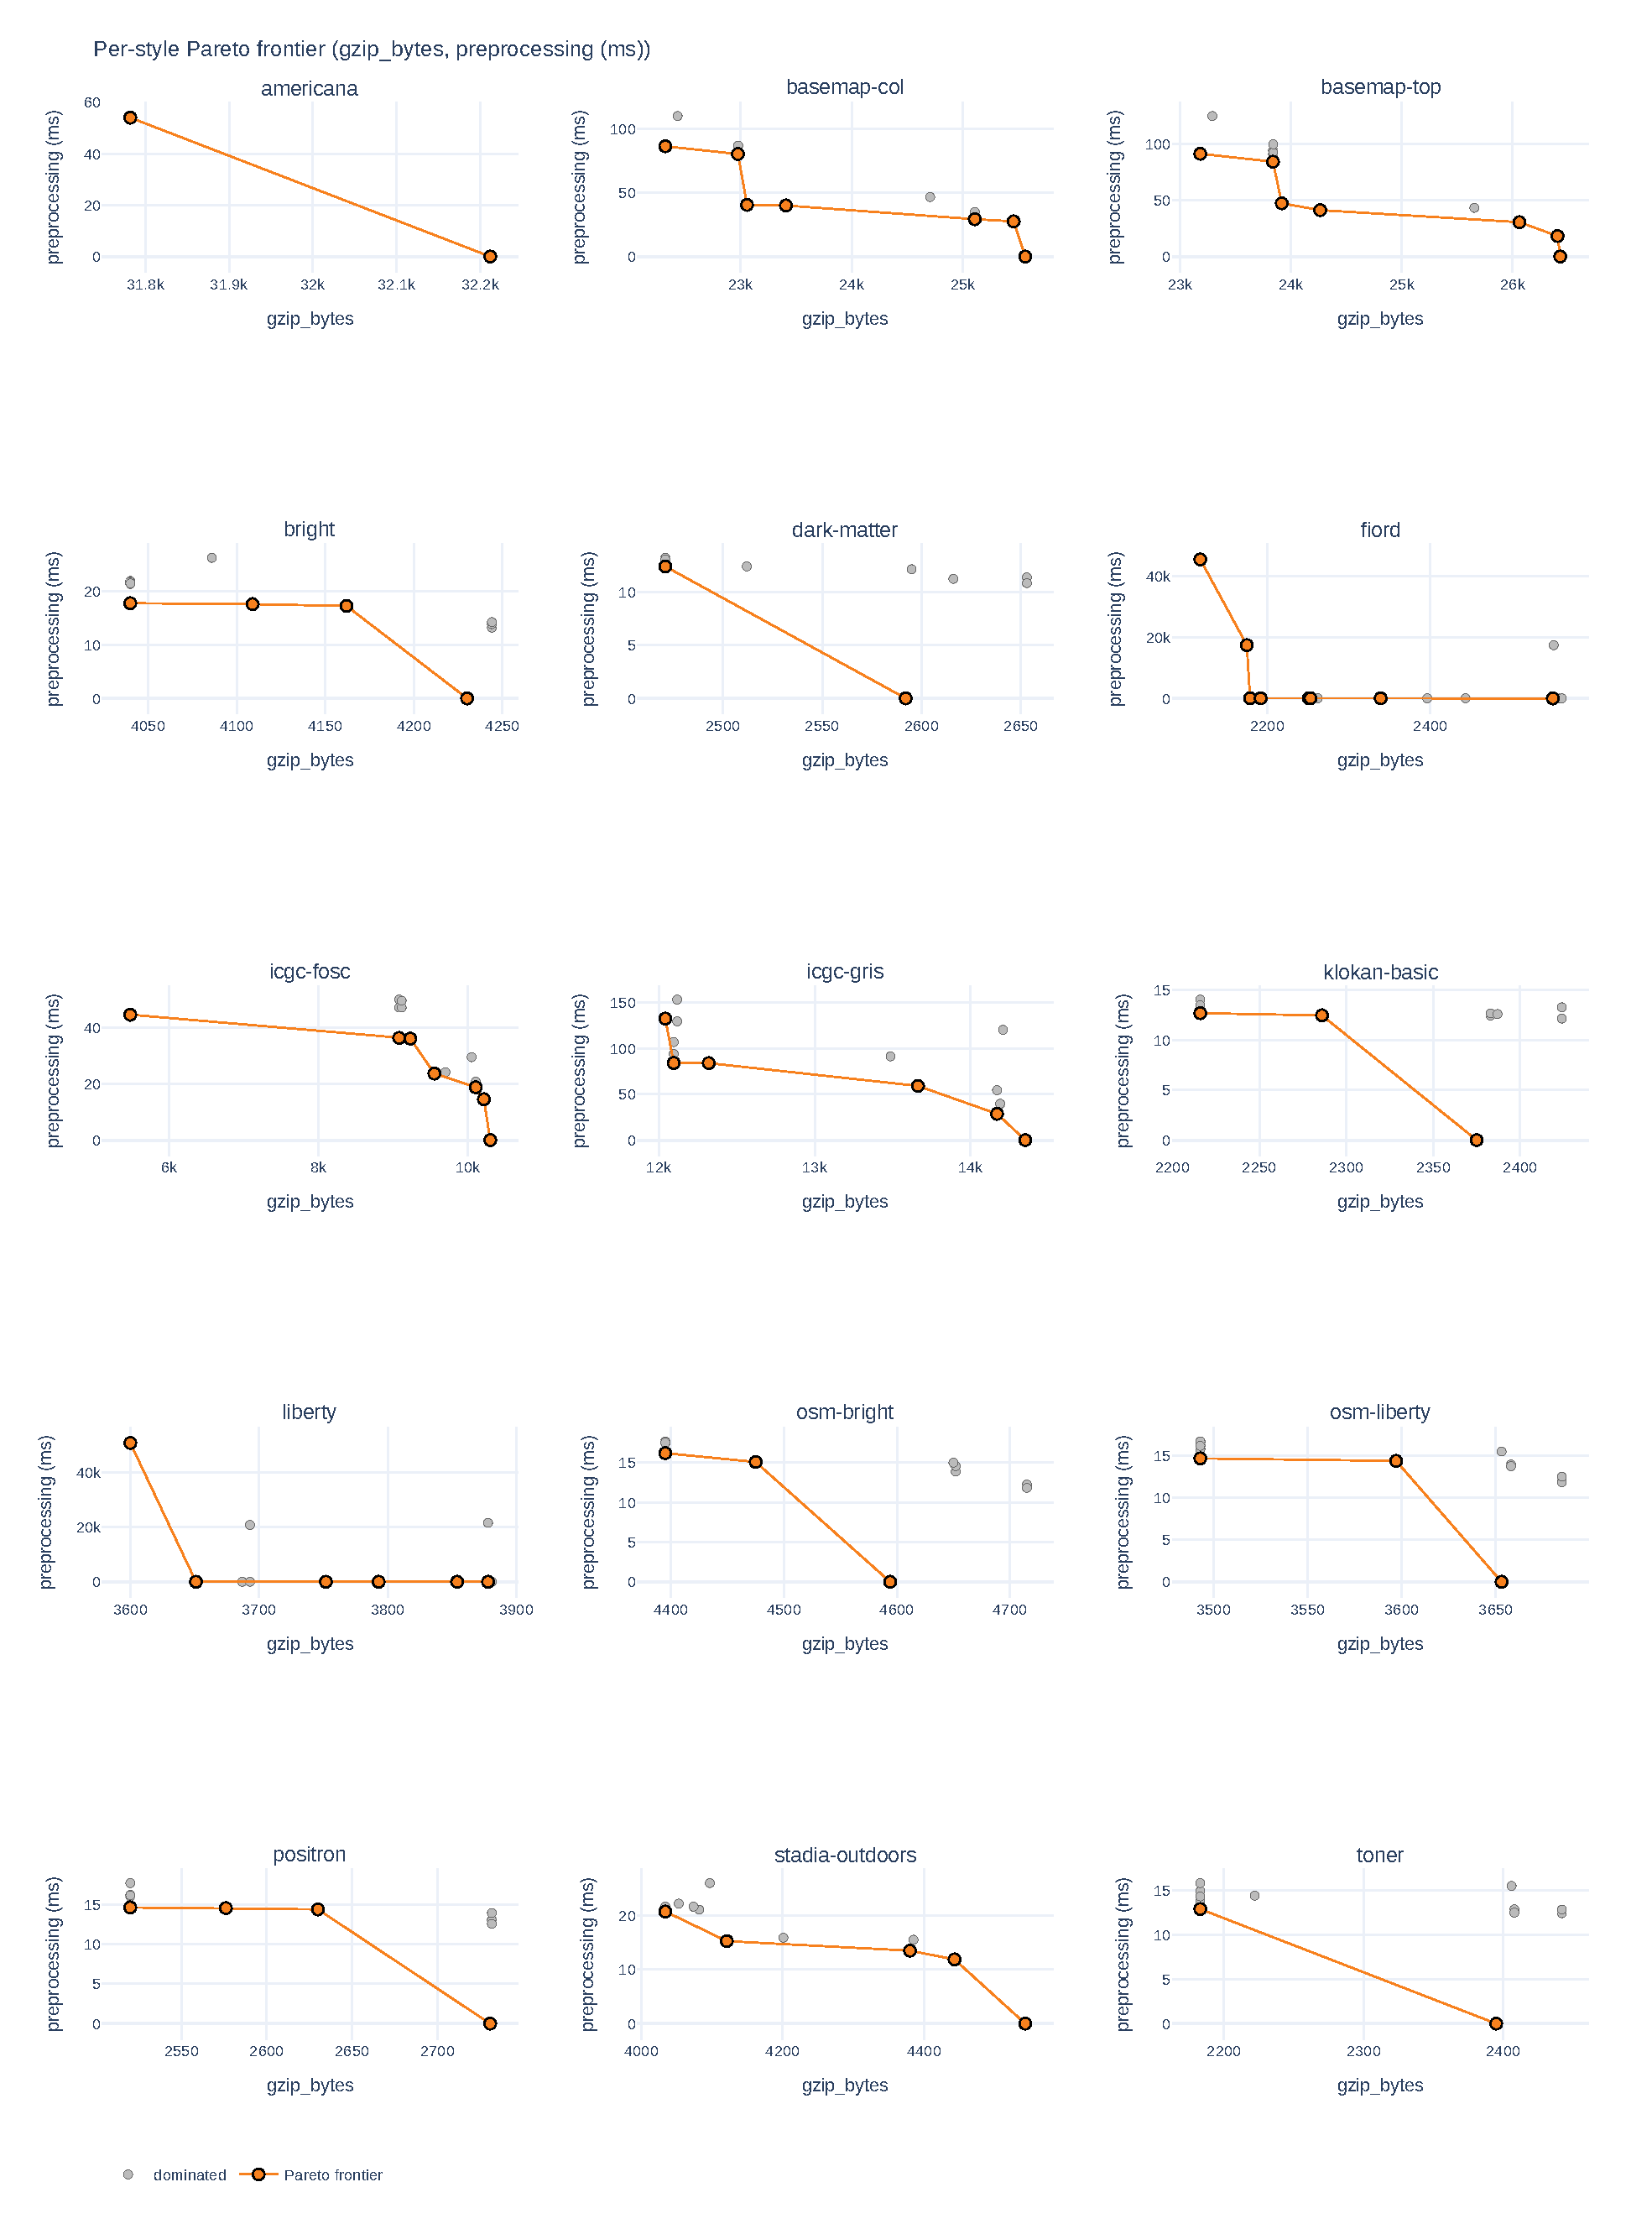
\includegraphics[width=\linewidth]{figures/pareto_per_style.pdf}
    \caption{Per-style Pareto frontier in \texttt{(gzip\_bytes, pass\_count)} space.
    Each point is a measured (style, variant) pair: cumulative-step variants populate the $x$-axis monotonically by construction and isolated-mode variants sit at \texttt{pass\_count}$=1$ with varying \texttt{gzip\_bytes}.
    Non-dominated points are highlighted; dominated points are rendered in grey.
    Generated from the \texttt{jsonl} output of the benchmark harness using the latest complete ablation session per style}
    \label{fig:pareto_per_style}
\end{figure}

The isolated-mode points are the operationally interesting part of the frontier: they reveal whether any single pass achieves a size reduction comparable to the full cumulative stack, and therefore whether a deployment that is willing to pay only for one pass has a clearly dominant choice.
The cumulative-trajectory points are monotonically non-increasing in \texttt{gzip\_bytes} by construction (every later step either shrinks or leaves the style size unchanged), so the cumulative portion of the frontier is simply the cumulative trajectory itself; the only way for a cumulative step to be dominated is if a later step reaches the same style size with fewer total passes, which is impossible by the \enquote{strictly additive} cumulative design.

\subsection{Discussion}\label{sub_pareto_discussion}

Across the benchmark corpus, baseline-to-final cumulative gzip reductions range from roughly \qty{3}{\percent} on already-compact styles (\texttt{bright}, \texttt{liberty}) to \qty{24}{\percent} on verbose styles (\texttt{klokan-basic}, \texttt{osm-bright}, \texttt{toner}), and the isolated-mode frontier exposes which single pass captures the largest share of that reduction per style.
The rendering-performance, decoding-latency, energy, and memory axes are not answered by this frontier because within-cell noise is of the same order as cross-variant signal (\cref{tab:pareto_noise}); decoding latency is instead addressed via isolated micro-benchmarks in \cref{tab:decode_throughput}, and the remaining axes are addressed at end-to-end granularity in \cref{sub_combined_ablation}.
The qualitative claims elsewhere in the thesis (\cref{sub_combined_discussion}'s mobile-battery discussion, \cref{sub_preprocessing_cost}'s cost model) remain authoritative on those axes because they operate on baseline-versus-full-pipeline aggregates where the effect size exceeds the noise floor.


\section{Visual Correctness Validation}\label{sec_visual_correctness}

A fundamental requirement of the optimiser is visual losslessness - the optimised output must satisfy the equivalence constraint formalised in \cref{sec_problem_statement}.
To validate this property, a systematic pixel-comparison test was conducted using pixelmatch, a pixel-level image comparison library that reports the number of differing pixels between two renderings with a configurable per-pixel colour tolerance.
For each of the 15 benchmark styles, the baseline and optimised renderings were compared at integer zoom levels 0-14 across all 18 scenarios, with both axis-aligned (no pitch, no bearing) and a fixed pitched view.
The comparison uses MapLibre GL~JS's Node-side software rasteriser rather than a GPU backend; this is a deliberate choice that trades realism for determinism: a software rasteriser produces bit-identical output across machines, whereas GPU backends diverge on subpixel rounding, fragment-shader precision, and mipmap selection even when all other inputs are held fixed.
Across all comparisons, pixelmatch reported zero differing pixels at a strict (zero-tolerance) threshold, confirming that every optimisations pass preserves visual identity on the software rasteriser.

Two caveats apply to this result.
First, the grid samples integer zoom levels and a small set of pitch and bearing settings; behaviour at fractional zoom levels and tilted camera trajectories is not directly asserted by pixelmatch.
The underlying optimisations invariants (overzoom-aware metadata refinement, painter's-order-pre\-serving layer merging) are, however, zoom-invariant by construction.
Second, the equivalence holds for the software rasteriser.
The benchmark harness runs the GPU backend (ANGLE/Vulkan) in parallel for performance measurement, and no GPU-only divergence appears in the benchmark traces, but the claim \enquote{pixel-exact on the GPU} is neither asserted nor required - style and tile transformations cannot introduce GPU-only divergences not already present in the software rasteriser, because both backends consume the same post-optimisations inputs.


\section{Threats to Validity}\label{sec_threats}

This section discusses potential threats to the validity of the experimental findings.

\paragraph{Internal validity}
All rendering benchmarks were conducted on a single hardware configuration (GPU model, CPU, memory) running a specific browser version with ANGLE/Vulkan as the graphics backend.
Performance characteristics may differ on other hardware or with different graphics backends (e.g., native OpenGL, DirectX, Metal).
The 15-run median was chosen to reduce measurement noise, but rare performance events (e.g., GPU thermal throttling, garbage collection pauses) may not be fully captured.
The caching proxy eliminates network variability but also prevents observation of real-world caching effects and \ac{CDN} behaviour.

\paragraph{External validity}
The evaluation is limited to MapLibre GL~JS; results may not transfer directly to other renderers such as Mapbox GL~JS, deck.gl, or native MapLibre implementations.
The tile data uses only OpenMapTiles and BasemapDE schemas; other schemas with different property distributions or geometry characteristics may yield different optimisations gains.
The 15 benchmark styles, while diverse, may not represent all style authoring patterns encountered in production deployments.

\paragraph{End-to-end data-level coverage}
The full pipeline - style optimisations through tile shaving to \ac{MLT} re-encoding - is benchmarked end-to-end on only 2 of the 15 styles (fiord and liberty).
This limitation arises because tile statistics at a sample rate of~1.0 require access to the underlying tile data, which is available only for \ac{OSM}-based tilesets accessed via a local \texttt{.mbtiles} file.
The remaining 13 styles either reference \ac{OSM} data through remote tile servers (where a full scan is impractical) or use the BasemapDE schema served via \acs{WMTS} (where the underlying data is not accessible for re-encoding).
The two styles that are benchmarked end-to-end represent different points in the complexity spectrum - fiord is a compact basemap (48 layers) and liberty is a detailed multi-source style (111 layers) - but they share the OpenMapTiles schema, so the property-reference profile driving the tile pruning advisory is similar for both.
Styles with substantially different property-reference patterns (e.g., BasemapDE styles that reference \texttt{funktion} and \texttt{objart} columns absent from OpenMapTiles) would produce different shaving advisories and potentially different cascade magnitudes.
The style-only results (Experiments~1-2) cover all 15 styles and are not affected by this limitation.

\paragraph{Construct validity}
Network conditions are simulated via a fixed bandwidth throttle rather than measured under real \ac{CDN} latency profiles.
The synthetic camera animations (zigzag, spiral, zoomdrill, pansweep, bearingspin) are designed to exercise diverse rendering workloads but may not capture typical user interaction patterns such as search-and-zoom workflows.

\paragraph{Statistical validity}
The selectivity estimation model assumes independence between filter predicates (\cref{eq:selectivity_compound}), which may not hold for correlated properties; map-style filters in practice do exhibit correlations (e.g.\ \texttt{class} and \texttt{subclass} in OpenMapTiles), so the estimator is a first-order approximation rather than a calibrated model, and selectivity-based reordering should be understood as a heuristic that produces a locally-good ordering rather than a provably-optimal one.
The 15-run median provides robustness against outliers but does not quantify sampling uncertainty on its own.
Bootstrap \qty{95}{\percent} confidence intervals (10\,000 resamples, percentile method) were computed over the per-(style, variant) measurement pools for \texttt{loadMs} and \texttt{fps}; the full table is provided in the supplementary data (\texttt{scripts/data/confidence\_intervals.csv}).
Error bars in the waterfall (\cref{fig:waterfall_loadMs}), marginal (\cref{fig:marginal_loadMs}), and rendering-metrics (\cref{fig:rendering_metrics_mlt}) figures represent these bootstrap \qty{95}{\percent} CIs.
Wilcoxon signed-rank tests (or Mann-Whitney~U where sample sizes differ) confirm that the full-pipeline load-time reductions are highly significant for both end-to-end styles (Fiord: \qty{374.9}{\milli\second}$\to$\qty{108.7}{\milli\second}, $p < 10^{-45}$; Liberty: \qty{493.0}{\milli\second}$\to$\qty{123.5}{\milli\second}, $p < 10^{-74}$).
Style-only effects on load time are smaller and, for individual styles, not consistently distinguishable from measurement noise - confirming the thesis's finding that the dominant load-time improvements come from tile shaving rather than style simplification.
The cumulative ablation design means that the reported marginal contribution of each pass depends on the ordering of preceding passes; a leave-one-out or fractional-factorial design would isolate each pass's standalone contribution more cleanly but was not run for cost reasons.
Tail metrics (p99 frame time, jank count) are particularly sensitive to sample size: with $n=15$ runs, the tail carries only a handful of informative samples per cell, and the reported numbers should be read as directional rather than conclusive.
The full-pipeline ablation performs thousands of pairwise comparisons across metrics, styles, scenarios, and ablation steps; no multiple-comparisons correction (Bonferroni, Benjamini-Hochberg) is applied, so individual per-cell \enquote{significant} differences should not be read as hypothesis tests, only as descriptive summaries.
